
%\newcommand{\DoNotLoadEpstopdf}{}
\documentclass[a4paper,12pt,spanish,twoside,openright]{book}
\usepackage{amsmath}
\usepackage[utf8]{inputenc}
\usepackage[spanish]{babel} %escribir con acentos sin necesidad de comandos
\usepackage{fancyhdr}

\usepackage[scaled]{uarial} %%%Tipo de letra a usar en el documento
\renewcommand*\familydefault{\sfdefault} %% Only if the base font of the document is to be sans serif
\usepackage[T1]{fontenc} %%%Tipo de letra a usar en el documento

\usepackage{epic}
\usepackage{eepic}
\usepackage{threeparttable}
\usepackage{amscd}
\usepackage{textgreek}
\usepackage{here}
\usepackage{graphicx}
%\usepackage{epstopdf}
\usepackage{caption}
\usepackage{subcaption}
\expandafter\def\csname ver@subfig.sty\endcsname{}
\usepackage{lipsum}
\usepackage{lscape}
\usepackage{tabularx}
 \usepackage{multirow}
\usepackage{ltablex}
%\usepackage{fontspec}
\usepackage{xcolor, color, soul}
\usepackage{geometry}
\usepackage{longtable}
\usepackage{glossaries}
\usepackage{makeidx}
\usepackage{acronym}
\usepackage{thumbpdf}
\usepackage[hidelinks]{hyperref}
\usepackage{wrapfig,booktabs} %%Para tablas flotantes
\usepackage{nicematrix}
\setcounter{MaxMatrixCols}{30}
\usepackage{fontawesome, xcolor}

\usepackage{stix} %%%Para figuras geométricas, como pentagono
\usepackage{nicematrix} %%%%Para las matrices
\usepackage{colortbl}
\usepackage{tikzsymbols}
\usepackage{tikz}
\usetikzlibrary{shapes.geometric} % Load the library for geometric shapes
%%%%%Fin


\geometry{a4paper, top=20mm, left=30mm, right=10mm, bottom=20mm,
headsep=10mm, footskip=12mm}

\definecolor{mygreen}{RGB}{0,100,0}  %%%Se usa más adelante para la tabla
\definecolor{myblue}{RGB}{0,55,100}
\makeglossaries
\makeindex

\usepackage{rotating} %Para rotar texto, objetos y tablas seite. No se ve en DVI solo en PS. Seite 328 Hundebuch
                        %se usa junto con \rotate, \sidewidestable ....


%%%%%%%%%Formaro títulos y subtítulos%%%%%%%%%%%%%%%%
\usepackage{lmodern}  %*****Para Número GRANDE fancy en cada caítulo*****
\usepackage{microtype}
\usepackage{titlesec}
%\usepackage{graphicx}
\usepackage{sectsty}
\chapterfont{\color{myblue}}  % sets colour of chapters
\sectionfont{\color{myblue}}  % sets colour of sections
\subsectionfont{\color{myblue}}  % sets colour of subsections
\subsubsectionfont{\color{myblue}}  % sets colour of subsections


%%%Para cuadro con número en cada capítulo
\usepackage{titlesec}
\titleformat{\chapter}[block]
{\color{myblue}\normalfont\bfseries}
   {\rlap{\makebox[\linewidth][r]{%
      \rotatebox[origin=c]{90}{% %%Ángulo CAPÍTULO
      \normalfont\color{myblue}\large%
      \textls[90]{\textsc{\chaptertitlename}}%
   }\hspace{10pt}% %%%Espacio entre "CAPÍTULO y el cuadro
   {\setlength\fboxsep{0pt}%
      \colorbox{myblue}{\parbox[c][3.0cm][c]{2.5cm}{% %%Tamaño de cuadro
      \centering\color{white}\fontsize{80}{90}\selectfont\thechapter}%
   }}}%
   }}
   {0pt}
   {\huge\parbox{\dimexpr\linewidth-3.5cm}}[{\medskip\color{myblue}\titlerule[2.5pt]}\color{myblue}\vskip2pt\titlerule]
    \usepackage{lipsum}

%%%linewidth-3.5cm} espacio entre título de cápituloo y cuadro con el número
%%%vskip2pt espacio entre la linea pequeña y la grande

%%%%{\color{myblue}\normalfont\bfseries} color título
%*****FIN Para Número GRANDE fancy en cada caítulo*****

%%%%%%%%%FIN Formaro títulos y subtítulos%%%%%%%%%%%%%%%%

%%%******Formato para tablas*******
\usepackage{pgfplotstable, booktabs}
\pgfplotsset{compat=1.8}
\usepackage{longtable}
\usepackage{array}

%%%****************Formato título figuras************
% Define a new caption style
\DeclareCaptionFormat{bold}{\textbf{#1#2}\textbf{#3}}
\captionsetup[figure]{format=bold, labelfont=bf}

\DeclareCaptionFormat{colored}{\color{myblue}\textbf{#1#2}\textbf{#3}}
\captionsetup[figure]{format=colored, labelfont=bf}

%%%%%%Labels top para las subfiguras
\captionsetup{font={bf,small},skip=0.25\baselineskip}
\captionsetup[subfigure]{font={bf,small}, skip=1pt, singlelinecheck=false}
%%%****************FIN Formato título figuras************

%%%%%%% Para Lista de figuras
\DeclareCaptionFormat{bold}{\textbf{#1#2}\textbf{#3}}
\captionsetup[table]{format=bold, labelfont=bf}
\DeclareCaptionFormat{colored}{\color{myblue}\textbf{#1#2}\textbf{#3}}
\captionsetup[table]{format=colored, labelfont=bf}


\renewcommand{\theequation}{\thechapter-\arabic{equation}}
\renewcommand{\thefigure}{\textbf{\thechapter-\arabic{figure}}}
\renewcommand{\thetable}{\textbf{\thechapter-\arabic{table}}}


\pagestyle{fancyplain}%\addtolength{\headwidth}{\marginparwidth}
\textheight22.5cm \topmargin0cm \textwidth16.5cm
\oddsidemargin0.5cm \evensidemargin-0.5cm%
\renewcommand{\chaptermark}[1]{\markboth{\thechapter\; #1}{}}
\renewcommand{\sectionmark}[1]{\markright{\thesection\; #1}}
\lhead[\fancyplain{}{\thepage}]{\fancyplain{}{\rightmark}}
\rhead[\fancyplain{}{\leftmark}]{\fancyplain{}{\thepage}}
\fancyfoot{}
\thispagestyle{fancy}%


%\addtolength{\headwidth}{0cm}
%\unitlength1mm %Define la unidad LE para Figuras
%\mathindent0cm %Define la distancia de las formulas al texto,  fleqn las descentra
%\marginparwidth0cm
%\parindent0cm %Define la distancia de la primera linea de un parrafo a la margen

%Para tablas,  redefine el backschlash en tablas donde se define la posici\'{o}n del texto en las
%casillas (con \centering \raggedright o \raggedleft)
\newcommand{\PreserveBackslash}[1]{\let\temp=\\#1\let\\=\temp}
\let\PBS=\PreserveBackslash

%Espacio entre lineas o interlineado del documento
\renewcommand{\baselinestretch}{1.5}

%Neuer Befehl f\"{u}r die Tabelle Eigenschaften der Aktivkohlen
\newcommand{\arr}[1]{\raisebox{1.5ex}[0cm][0cm]{#1}}

%Neue Kommandos
\usepackage{Befehle}
%Inicio del documento. Tener en cuenta que hay archivos auxiliares

%%%Para los marcadores más adelante de las gráficas
\definecolor{falured}{rgb}{0.5, 0.09, 0.09} %%2.0%
\definecolor{emerald}{rgb}{0.31, 0.78, 0.47} %%%3.5%
\definecolor{goldenpoppy}{rgb}{0.99, 0.76, 0.0} %%5.0
\definecolor{deepmagenta}{rgb}{0.8, 0.0, 0.8}  %%7.0%

%%%%%%%Para hacer tabla Pad tipo usado en el Factor Lambda Chap 3
\usepackage{environ}
\newcommand{\TablePad}{\vspace{-0.2cm}}
\NewEnviron{EntriesTableDuration}{
\TablePad
\begin{tabularx}{\textwidth}{@{}p{0.10\textwidth}@{\hspace{0.02\textwidth}}p{0.88\textwidth}@{}}
  \BODY
\end{tabularx}
\TablePad
}
\NewEnviron{EntriesTableYear}{
\TablePad
\begin{tabularx}{\textwidth}{@{}p{0.05\textwidth}@{\hspace{0.01\textwidth}}p{0.94\textwidth}@{}}
  \BODY
\end{tabularx}
\TablePad
}
%%%%Fin formato%%%

%%%%Para símbolo de aprox igual
\DeclareFontFamily{U} {cmsy}{}
\DeclareFontShape{U}{cmsy}{m}{n}{
  <-6> cmsy5
  <6-7> cmsy6
  <7-8> cmsy7
  <8-9> cmsy8
  <9-10> cmsy9
  <10-12> cmsy10
  <12-> cmsy12}{}
\DeclareSymbolFont{Xcmsy} {U} {cmsy}{m}{n}
\DeclareMathSymbol{\Xapprox}{\mathrel}{Xcmsy}{25}
%%%Fin


%%Colocar "[numero]." punto después de número y espacio en bibliografía
\usepackage[numbers]{natbib}
\makeatletter
%\renewcommand{\@biblabel}[1]{\makebox[1em][l]{#1.}} Solo el número
\renewcommand{\@biblabel}[1]{[#1].}
\makeatother

%%%%Símbolo derivda parcial para monocapas
\DeclareMathSymbol{\partial}{\mathord}{letters}{"40}


\begin{document}

\pagenumbering{roman}

%%\newpage
%\setcounter{page}{1}
%%%%%%%Portada%%%%%%%
\begin{center}
\begin{figure} % supposedly places it here ...
    \centering
	
\includegraphics[width=0.79\linewidth]{porta_cover/logo_full.eps}
\end{figure}

\thispagestyle{empty} \vspace*{2.0cm} \textbf{\huge
Título de la tesis  o trabajo de investigaci\'{o}n}\\[4.0cm]
\Large\textbf{Ubeiden Cifuentes Samboni}\\[4.0cm]
\small Escuela de Química, Facultad de Ciencias Qímicas\\ Departamento Química Biolólogica Ranwel Caputto\\
Centro de Invistigación de Química Biológica de Córdoba\\
Universidad Nacional de Córdoba\\
Córdabo, Argentina\\
2024
\end{center}

\newpage{\pagestyle{empty}\cleardoublepage}
%%%%%%%Portada Pag2%%%%%%%
\newpage
\begin{center}
\thispagestyle{empty} \vspace*{0cm} \textbf{\huge
T\'{\i}tulo de la tesis  o trabajo de investigaci\'{o}n}\\[3.0cm]
\Large\textbf{Ubeiden Cifuentes Samboni}\\[3.0cm]
\small Tesis o trabajo de grado presentada(o) como requisito parcial para optar al
t\'{\i}tulo de:\\
\textbf{doctor en ciencias químicas}
Director:\\
Dr. Guillermo Gabriel Montich\\[2.0cm]
L\'{\i}nea de Investigaci\'{o}n:\\
Nombrar la l\'{\i}nea de investigaci\'{o}n en la que enmarca la tesis  o trabajo de investigaci\'{o}n\\
Grupo de Investigaci\'{o}n:\\
Nombrar el grupo en caso que sea posible\\[2.5cm]
Universidad Nacional de Colombia\\
Facultad, Departamento (Escuela, etc.)\\
Ciudad, Colombia\\
2024\\
\end{center}


\renewcommand{\tablename}{\textbf{Tabla}}
\renewcommand{\figurename}{\textbf{Figura}}
\renewcommand{\listtablename}{Lista de tablas}
\renewcommand{\listfigurename}{Lista de figuras}
\renewcommand{\contentsname}{Contenido}


% Tabla de contenidos
\cleardoublepage
\addcontentsline{toc}{chapter}{Contenido}
\tableofcontents


%\newcommand{\clearemptydoublepage}{\newpage{\pagestyle{empty}\cleardoublepage}}
\cleardoublepage
\addcontentsline{toc}{chapter}{Lista de figuras} % para que aparezca en el indice de contenidos
\listoffigures % indice de figuras

\cleardoublepage
\addcontentsline{toc}{chapter}{Lista de tablas} % para que aparezca en el indice de contenidos
\listoftables % indice de tablas

\cleardoublepage
\addcontentsline{toc}{chapter}{Lista de abreviaturas} 
\chapter*{Lista de abreviaturas}

%--- Acronyms -----------------------------------------------------------------%
% \acrodef{label}[acronym]{written out form} % acronym syntax
%\acrodef{etacar}[$\eta$ Car]{Eta Carinae}   % acronym example
%--- Acronyms -----------------------------------------------------------------%
% how to use acronyms:
% \ac = use acronym, first time write both, full name and acronym
% \acf = use full name (text + acronym)
% \acs = only use acronym
% \acl = only use long text
% \acp, acfp, acsp, aclp = use plural form for acronym (append 's')
% \acsu, aclu = write + mark as used
% \acfi = write full name in italics and acronym in normal style
% \acused = mark acronym as used
% \acfip = full, emphasized, plural, used
%--- Acronyms -----------------------------------------------------------------%


\begin{acronym}[SDS-PAGE] % Replace 'EC' with the longest acronym
    \setlength{\itemsep}{2pt} % Adjust the vertical spacing between items
     %%\acro{}[]{}
        \acro{ec}[EC]{extracelular}
        \acro{tm}[TM]{transmembrana}
        \acro{ic}[IC]{intracelular}
        \acro{acn}[ACN]{acetonitrilo}
        \acro{hplc}[HPLC]{cromatografía líquida de alta presión}
        \acro{bam}[BAM]{microscopía de ángulo de Brewster }
        \acro{mbp}[MPB]{proteína de unión a maltosa }
        \acro{tev}[TEV]{virus del grabado del tabaco}
        \acro{ecoli}[\emph{E. coli}]{\textit{Escherichia coli}}
        \acro{iptg}[IPTG]{isopropil $\beta$-D-1-tiogalactopiranósido}
        \acro{popc}[POPC]{palmitoil-oleoil-fosfatidilcolina}
        \acro{popg}[POPG]{palmitoil-oleoil-fosfatidilglicerol}
        \acro{dppc}[DPPC]{dipalmitoilfosfatidilcolina}
        \acro{lb}[LB]{lysogeny broth}
        \acro{pbs}[PBS]{buffer fosfato-salino}
        \acro{pdb}[PDB]{Protein Data Bank}
        \acro{pmsf}[PMSF]{fluoruro de fenilmetilsulfonilo}
%        \acro{sds}[SDS]{dodecil sulfato de sodio }
        \acro{sds}[SDS-PAGE]{electroforesis de gel en poliacrilamida con dodecil sulfato de sodio}
        \acro{Trix}[Trix]{tris (hidroximetil) aminometano}
        \acro{DO$_{600}$}[DO$_{600}$]{densidad óptica a 600 nm}
        \acro{fplc}[FPLC]{cromatografía líquida rápida de proteínas}
        \acro{rpm}[rpm]{revoluciones por minuto}
        \acro{cv}[CV]{volúmenes de columna}
        \acro{uv}[UV]{ultravioleta}
        \acro{dtt}[DTT]{DL-Ditiotreitol}
        \acro{tfa}[TFA]{ácido trifluoroacético}
        \acro{em}[EM]{espectrometría de masas}
        \acro{meoh}[MeOH]{metanol}
        \acro{chcl3}[CHCl$_3$]{Cloroformo}
        \acro{tr}[t$_R$]{tiempo de retención}
        \acro{atr}[ATR]{reflectancia total atenuada}
        \acro{ftir}[FTIR]{infrarrojo por transformada de Fourier}
        \acro{sncad}[SNCAD]{sistema nacional de computación de alto desempeño}
        \acro{dm}[DM]{dinámica molecular}
        \acro{pdb}[PDB]{protein data bank}
        \acro{rmn}[RMN]{resonancia magnética nuclear}
        \acro{criomicro}[cryo-EM]{microscopía electrónica en condiciones criogénicas}
        \acro{le}[LE]{líquido expandido}
        \acro{lc}[LC]{líquido condensado}
        
        
        
\end{acronym}
 % Include your list of abbreviations

%\include{Resumen}%\newcommand{\clearemptydoublepage}{\newpage{\pagestyle{empty}\cleardoublepage}}¸
\pagenumbering{arabic}
\chapter{Introducción}

\section{Membrana biológica}

La membrana celular, también llamada membrana plasmática es la barrera física entre la célula y el ambiente exterior de la misma.  Ésta tiene la característica de actuar como una estrucura semipermeable y esta compuesta principalmente de una gran variedad de lípido y proteína embedidas. Sin embargo, esta barrera física no solamente se limita a permitir la entra y/o salida de componentes en la célula, sino que tiene gran relevancia en varios procesos celulares como son la tracción celular y señalización celular \hl{cell-signalling}. 


Las propiedades mecánicas de la membrana, como la tensión superficial y el módulo de elasticidad estan extrechamente relacionadas a la función celular. Estas propiedades son moduladas por el citoesqueleto y una red de proteínas filamentosas (o escleroproteínas)  ancladas a la membrana vía proteínas integrales de membrana \cite{Vinogradova2002, Karagoz2021}.
%%https://theses.hal.science/tel-01685239/preview/KURAUSKAS_2017_archivage.pdf

\section{Integrinas}

Las integrinas son parte de una gran familia de receptores de membrana de paso único. Estan compuestas por dos subunidades, en cada subunidad se distinguen tres dominios, un gran dominio \ac{ec} (800 amino ácidos), una $\alpha$ hélice \ac{tm} (20 amino ácidos) y un corto dominio \ac{ic} o citoplasmático mayoritariamente no estructurado (ref). Se conocen cerca de 25 miembros de integrinas (18 subunidades - $\alpha$  y 8 subunidades - $\beta$) (ref), cada miembro tiene sitios de reconocimientos diferentes a unión de ligandos, asi como también interaccionan con diferentes proteínas de adhesión.


Las integrinas son receptores fisiológicamente relevantes que median la interacción celular controlada por ligandos y mensajes intra- e intercelulares, transducen señales bidireccionalmente entre el interior y el exterior celular.


Podemos observar la secuencia primaria correspondiente al péptido $\alpha$IIb desde N al C-terminal que incluye un pequeño loop extracelular (10 resíduos), en rojo se resalta el segmento o dominio \ac{tm} (28 resíduos) y la cola citoplamática, en \textbf{negrilla} se resalta región con estructura secundaria $\alpha$-hélice,  de forma similar en la Figura x se aprecia la secuencia primaria para el péptido $\beta$3


Como se observa $\beta$3 tiene un segmento \ac{ic} mucho más largo que $\alpha$IIb
%%Acá hablan de una base de datos de solo TM \url{https://onlinelibrary.wiley.com/doi/epdf/10.1002/pro.4318}
%%y hay info del tilt angle


\section{Motivación y objetivo de la tesis}
\chapter{Metodología}\label{metod}

\section{Metodología experimental}

\subsection{Plásmidos, reactivos, equipos y materiales}
La secuencia de los segmentos \ac{tm}-\ac{ic} de los péptidos $\alpha$IIb y $\beta$3 fueron donados por el laborario del Dr. Jun Qin {ref}. Cada plásmido fue clonado en la cepa de bacteria \ac{ecoli} DH5$\alpha$. La incorporación de los plásmidos fue verificada usando un kit de purificación de ADN "Wizard Plus SV Miniprep" (Promega, Madison, WI, USA). Ampicilina \hl{(escribir de donde se obtuvo, referencia)}   \ac{iptg} fue adquirido en Gentbiotech. Las  columnas  de Sefarosa Ni HisTrap HP  5 mL y de desalado PD-10 fueron adquiridas en GE Healthcare (Cat. 71-5027-68 Cat. 17085101, respectivamente). Para el \ac{hplc} se usó en equipo Agilent Technologies 1260 Infinity con detector de arreglo de diodos y longitud de onda múltiple (DAD VL), equipado con software ChemStation/Open LAB; columna Ultisil XB-C4, 5 $\mu$m, 300 Å, 4.6x250 mm, cat.00216-33043 (Welch SKU. H00216-33043, USA). Las membranas de celulosa (Dialysis Tubing, Benzoylated, poro de 2000 MWCO) fueron adquiridas en SIGMA. La concentración de proteína fue determina en espectrofotómetro Varian 2300, (Palo Alto, CA, USA). Las \ac{sds} y disoluciones amortiguadoras fueron preparadas usando agua grado Milli-Q tipo 1. Los análisis de \ac{em} se realizaron en un espectrómetro de masas ESI-Qq-TOF (Bruker). 
Los lípidos \ac{popc}, \ac{popg}, \ac{dppc}, fueron adquiridos en Avanti Polar, USA; el  \ac{chcl3}, \ac{acn} y \ac{meoh} grado \ac{hplc} en la firma Merck, Alemania.

\subsection{Extracción y clonación de plásmidos}
%%Para redactar ver parte se soporte del paper Qin & Jun
%%%https://www.sciencedirect.com/science/article/pii/S0168165622003042?via%3Dihub
%%% diagrama del plasmido https://sci-hub.se/10.1080/10409230490514008
Ambos plásmidos pMAL-c2 (New England Biolabs, Inc., Beverly, MA) fueron replicados por separado en la cepa \emph{E. coli} DH5$\alpha$ (ver \textbf{protocolo} \ref{Protocolo Plasmido}). Este vector contenía la secuencia que codifica cada péptido y la \ac{mbp} para facilitar un primer paso de purificación que llamaremos "proteína fusión". Entre el N-terminal de la \ac{mbp} y el C-terminal de cada péptido, hay una etiqueta de hexahistidina o His$_{6}$-\emph{tag} y sitio de corte para la proteasa del \ac{tev} que permiten separar cada secuencia de interés en dos pasos de purificación (\textbf{figura} \ref{fig:plasmido}). Además, posee la secuencia \emph{amp$^r$} que permite seleccionar bacterias que incorporen el plásmido con ampicilina. Todos los medios y material utilizado, asi como el agua Milli-Q fueron esterilizados en autoclave por 30 minutos a 1 atm de presión y 120°C.

%%%%%%%%%%%%%%%%%%%%% Fig plasmido %%%%%%%%%%%%%%%%%%%%%%%%
\begin{figure}[h] % supposedly places it here ...
    \centering
	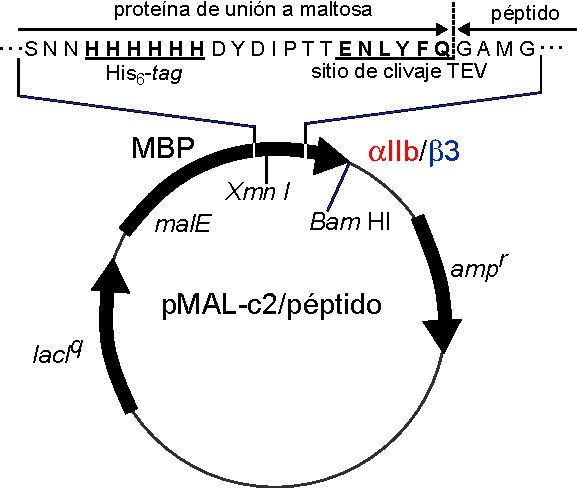
\includegraphics[width=0.79\linewidth]{fig/01_expe/pmal_c2.pdf}
	\caption[Esquema plásmido pMAL-c2 - $\alpha$IIb/$\beta$3]{Esquema plásmido pMAL-c2 - $\alpha$IIb/$\beta$3. Figura adaptada de Vector Database por \href{https://www.addgene.org/}{addgene.org} (2023). Extraído de \href{https://www.addgene.org/vector-database/3506/}{https://www.addgene.org/vector-database/3506/}.
        \index{plasmido}}
    \label{fig:plasmido}
\end{figure}
%%%%%%%%%%%%%%%%%%%%% Fin %%%%%%%%%%%%%%%%%%%%%%%%


\subsection{Expresión y purificación proteína fusión}\label{sec:expre_akta}

Una vez clonada cada secuencia \ac{tm}-\ac{ic} de los plásmidos $\alpha$IIb y $\beta$3 se expresó la proteína fusión en una cepa de bacterias \emph{E. coli} BL21(DE3), ver Protocolo \ref{Protocolo_Fusion}. Posteriormente se lisaron las bacterias y se purificó la proteína por afinidad a níquel en \ac{fplc}. 
Se cuantificó cada proteína fusión por espectrofotometría \ac{uv} teniendo en cuenta los coeficientes de absortividad molar, {\Large{$\varepsilon$}} a 280 nm: {\Large{$\varepsilon$}}$_{\alpha \text{IIb}}$ = 85830 M$^{\text{--1}}$ \, cm$^{\text{--1}}$, {\Large{$\varepsilon$}}$_{\beta\text{3}}$ = 83310 M$^{\text{--1}}$ \, cm$^{\text{--1}}$;
 valores obtenidos de \url{https://web.expasy.org/protparam/}. El rendimiento de cada \textbf{proteína fusión} fue de 10 y 15 mg/L cultivo para $\alpha$IIb y $\beta$3,  respectivamente.

Por otra parte también se expresó y purificó la proteasa \ac{tev} en nuestro laboratorio,  para ello, se tomó el plásmido de la proteasa TEV (donada por el laboratorio del Dr. Ernesto Ambroggio), se inoculó en la cepa \emph{E. coli} BL21(DE3) y se purificó por afinidad a níquel.

\subsection{Clivaje y diálisis}

La proteína fusión fue incubada con la proteasa \ac{tev} y se dejó a 30°C por $\Xapprox$ 48 horas. Se centrifugó y  se recuperó el sobrenadante el cual se dialisó en membranas de celulosa contra agua con agitación constante a 4°C. El contenido de las membranas se centrifugó en tubos eppendorf a 13000 \ac{rpm} por 10 minutos, \textbf{precipitando el péptido transmembrana} (en el sobrenadante se separó \ac{mbp}, \ac{tev} y proteína fusión sin cortar). El pellet se resuspendió \ac{acn}:H$_{2}$O 40:60 (vol/vol) con \ac{tfa}, consultar Protocolo \ref{Protocolo_TEV} para más detalle.

\subsection{Repurificación por \ac{hplc}}
Se realizaron múltiples cromatografías inyectando 1.0 mL de muestra bajo las siguientes condiciones cromatográficas:


%%%%%%%%%%%%%%%%%%%%% Tabla pequeña %%%%%%%%%%%%%%%%%%%%%%%%
\begin{wraptable}{r}{3.5cm}
\vspace{-0.8cm} %%%Posiciona a una altura en la hoja
\centering
    \caption{\\Gradiente HPLC.}\label{tab:hplc_gradiente}
    \begin{tabular}[t]{ccc}%%%c: center, l: leaft, r:right
     \toprule  % <-- Toprule here
      {Min}  & {A\%} & {B\%}\\
      \hline
        0       &  60    & 40  \\
        7       &  58    & 42 \\
        8       &  54    & 46  \\
        10      &  48    & 52 \\
        15      &  44    & 56  \\
        20      &  40    & 60 \\
        25      &  36    & 64  \\
        30      &  32    & 68 \\
        35      &  28    & 72  \\
    \textbf{40} & \textbf{24}    & \textbf{76} \\
        45      &  15    & 85  \\
        50      &  5     & 95 \\
        55      &  0     & 100  \\
      \bottomrule % <-- Bottomrule here
    \end{tabular}
    \vspace{-0.5cm} %%%Posiciona texto debajo tabla
    \end{wraptable} 
%%%%%%%%%%%%%%%%%%%%% Fin %%%%%%%%%%%%%%%%%%%%%%%%

\begin{tabularx}{\textwidth}{@{}p{0.20\textwidth} p{0.85\textwidth}@{}}
Fase móvil A: & 40\% H$_{2}$O(+0.1\% \ac{tfa}) \\
Flujo:              & 1.0 mL/min        \\ 
Temperatura:        & 40ºC              \\
Presión máxima:     & 210 bar           \\
Detector UV:        & 280 nm            \\
Inyección:          & 1.0 mL (manual)     \\
Fase móvil B:   & 100\% \ac{acn}(+0.1\% \ac{tfa}) \\
\end{tabularx}


Se colectaron todas fracciones del cromatograma según el gradiente de la \textbf{tabla} \ref{tab:hplc_gradiente} y se verificó la pureza por geles \ac{sds} y por \ac{em}.  Los péptidos purificados fueron solubilizados en \ac{acn}:H$_2$O 67\%/33\% (vol/vol); la concentración se determinó por absorbancia \ac{uv} teniendo en cuenta los {\Large{$\varepsilon$}} a 280 nm para cada péptido: {\Large{$\varepsilon$}}$_{\alpha \text{IIb}}$ = 16500 M$^{\text{--1}}$ cm$^{\text{--1}}$, {\Large{$\varepsilon$}}$_{\beta \text{3}}$ = 13980 M$^{\text{--1}}$ cm $^{\text{--1}}$. La remoción de \ac{tfa} y verificación de estructura secundaria de los péptidos se realizó por espectroscopía \ac{ftir}-\ac{atr}. El rendimiento final fue de 400 $\mu$g/L cultivo para $\alpha$IIb y 600 $\mu$g/L para $\beta$3. Se fraccionaron y almacenaron a -20°C para su posterior uso (ver Protocolo \ref{Protocolo_HPLC}).

\subsection{Electroforesis en gel y \ac{em}}

%%https://core.ac.uk/download/pdf/71054185.pdf
La pureza de ambos péptidos fue confirmada por geles SDS-PAGE y \ac{em}. Al tratarse de péptidos altamente hidrofóbicos se prepararon geles de poliacrilamida al 18\% en condiciones desnaturalizantes con \ac{sds}, junto con las muestras se sembró un marcador de peso molecular como referencia. La electroforesis se corrieron a 125 V y 4°C.

Se prepará una solución 100 $\mu$M de péptido en 67\%/33\% (vol/vol) + 0.1\% ácido fórmico y se inyectó en el espectrómetro de masas. El espectro fue adquirido en modo ion positivo desde 250 a 30000 m/z, con flujo de inyección de $\mu$L/min. El procesamiento de los datos se realizó en el software Data Analysis de Bruker \hl{REF}. Se promediaron dos cromatogramas, se procesó por deconvolución de la carga después de haber sustraído la línea base y se realizó un suavizado para obtener un cromatograma de alta resolución relación masa-carga m/z. Alternativamente los datos fueron post-procesados usando el Algoritmo de Máxima Entropía para obtener un espectro de masa neutra. Para ambos péptidos se obtuvo la masa esperada para los monómeros.

\subsection{Experimentos de monocapas de Langmuir}

Los experimentos de monocapas de Langmuir fueron realizados a temperatura ambiente (20°C). Todos los stock de soluciones de lípidos fueron preparadas en acetonitrilo:metanol. Las monocapas se realizaron en una unidad de control de Monofilmmeter (con Film Lift, Mayer Feintechnique, Alemania). La presión superficial ($\pi$) se midió usando el método de Wilhelmy con una placa Platinized-Pt y el potencial superficial ($\Delta$V) se detectó mediante el uso de una placa ionizante de $^{241}$Am. Los datos fueron registrados de forma continua y simultánea con un registrador X-YY de doble canal. El área superficial total de la cuba de Teflón fue de 80 cm$^2$ con capacidad de $\Xapprox$ 75 mL para la subfase (PBS 20 mM, NaCl 100 mM a pH 7.4). Para los péptidos puros se evaporó el solvente ACN:H$_2$O con flujo de nitrógeno (N$_{2 \text{(g)}}$) y se realizaron al menos 3 lavados con CHCl$_3$:MeOH 2:1 (vol/vol). La monocapa formaron directamente sembrando 0.5 nmoles de péptido solución CHCl$_3$:MeOH  en la subfase usando una jeringa Hamilton. Tanto para la isoterma del lípido puro como para las mezclas con péptidos se procedió de forma similar y se esperó por 8 minutos antes de empezar la compresión para dar tiempo a la evaporación del solvente y posteriormente se empezó a comprimir a razón fija de \hl{xx} cm$^2$/min. Antes de sembrar las muestras se realizaron los respectivos controles, para la superficie limpia y los disolventes de las muestras, en donde no se observó actividad superficial. Cada experimento se realizó por triplicado de forma independiente y se prepararon soluciones stock frescas de cada lípido cerca al momento de utilizarse.

Se realizaron ciclos de compresión-expansión, inicialmente las barreras se fijaron en 60 cm$^2$, se inició la compresión hasta llegar a los $\Xapprox$ 13 cm$^2$ y se expandió hasta los $\Xapprox$ 60 cm$^2$ y así se repitió tres veces para cada muestra.

%%%%Chequear este  \href{https://core.ac.uk/download/pdf/82003288.pdf}{link} para la discusión \href{https://reader.elsevier.com/reader/sd/pii/S0005273604000938?token=5AF045228C4131E3A6448735F6B35CEDFBE3138E3BF1D45DB2953593E8269614FD38EE1558AB7F2BBA9791113A5E77C5&originRegion=eu-west-1&originCreation=20230505170518}{otro link}

\subsection{Análisis de datos}

El procesamiento de los datos experimentales se realizó con código Python haciendo uso de las librerias  numpy (\hl{ref}), pandas (\hl{ref}). Todos los gráficos fueron generados con las librería Matplotlib (\hl{ref}).

%%Las imágenes de BAM fueron procesadas con el software Fiji (ref).

\section{Metodología computacional}

\subsection{Preparación de los sistemas}

%%https://ri.conicet.gov.ar/bitstream/handle/11336/80885/CONICET_Digital_Nro.9055fee5-f857-4ecf-960e-a5a4295f5f16_A.pdf;jsessionid=2EEA4DCEADDE4525930B5972D0F151B6?sequence=2

%%%https://ricabib.cab.cnea.gov.ar/952/1/1Cometto.pdf

%%https://bibliotecadigital.exactas.uba.ar/download/tesis/tesis_n6871_Bringas.pdf 
Las simulaciones de dinámica molecular grano grueso (CG-MD) se realizaron usando el campo de fuerza Martini 2 \hl{REF}, las coordenadas péptidos transmembrana fueron tomadas de la base de datos Protein Data Bank (PDB: 2KNC \hl{REF}. Se usó el servidor CHARMM-GUI \hl{REF} para emdidir el dímero $\alpha$IIb/$\beta$3 en una bicapa, el cual implementa el programa INSANE (INSert membrANE) que convierte las partículas del modelo atomístico a grano grueso \hl{REF}.
Los dinámicas se produjeron con los recursos de cómputo del \ac{sncad} usando los cluster Mendieta, Serafín (CCAD-UNC, \url{http://ccad.unc.edu.ar}) y con el cluster Create del King’s College London (\url{https://docs.er.kcl.ac.uk/CREATE/access/}). Se aplicó una red elástica aplicada (ElNeDyn) \hl{REF} sobre las partículas C$_\alpha$ de cada péptido usando una distancia \textit{cutoff} de 7 $\AA$, el dímero $\alpha$IIb/$\beta$3  fue insertado en 4 membranas de diferente composición cada una compuesta de 250 lípidos por hemicapa (POPC, POPG, POPC:POPG 70:30 (PCPG), DPPC). El sitema lípido-peptido fue hidratado con el modelo de agua polarizable (PW) \hl{REF}, finalmente se agregó NaCl hasta una concentración 0.15 M. El sistema se minimizó por 1000 pasos usando el método \textit{step desendent} \hl{REF}, posteriormente se equilibró en condiciones NPT por 5 ns aplicando posiciones de restricción para los $C_\alpha$ en las regiones con $\alpha$ hélice. Se usó el termostato de Berendsen \hl{REF} y el barostato Parrinello-Rahman \hl{REF} para mantener la temperatura a 320 K (excepto el sistema con DPPC que se simuló a 340 K) y la presión a 1 atmósfera con acoplamiento semi-isotrópico con una compresibilidad de 4.5 x 10$^{\text{--5}}$ bar$^{\text{--1}}$. Las interacciones eletrostáticas de largo alcance fueron incorporadas através del método de partículas de  Ewald con un \textit{cutoff} de 1 nm \hl{REF}. El mismo \textit{cutoff} se aplicó para las interacciones Lennard-Jones.


%%%REF insane: Wassenaar, T. A., Ingolfsson, H. I., Bockmann, R. A., Tieleman, D. P. & Marrink, S. J. Computational lipidomics with insane: A 
%%versatile tool for generating custom membranes for molecular simulations. J. Chem. Teory Comput. 11, 2144–2155 (2015).

%%%REF eledyn Lopez, C. A. et al. Martini coarse-grained force feld: Extension to carbohydrates. J. Chem. Teory Comput. 5, 3195–3210 (2009).
%%45. Periole, X., Cavalli, M., Marrink, S. J. & Ceruso, M. A. Combining an elastic network with a coarse-grained molecular force feld: 
%%Structure, dynamics, and intermolecular recognition. J. Chem. Teory Comput. 5, 2531–2543 (2009).


\subsection{Análisis de trayectorias}

El análisis de trayectorias se realizó con el paquete GROMACS, la librería MDAnalisys \hl{REF} con código en bash y python haciendo uso de algunas librerías como Numpy \hl{REF}, Pandas \hl{REF}. Los gráficos fueron generados con las librerías Matplotlib \hl{REF}, Seaborn \hl{REF}. La visualización de las trayectorias se realizó con el software VMD \hl{REF}.
\chapter{Generalidades, expresión y purificación de segmentos transmembrana de integrinas $\alpha$IIb/$\beta$3}\label{chap:pept}

Como se mencionó en la introducción (sección  \hl{link a intro}) las integrinas de las subfamilias $\beta$1, $\beta$2 y $\beta$3 juegan un rol muy importante en muchos procesos biológicos relacionados con células epiteliales, endoteliales, leucocitos, fibroplastos y plaquetas, por lo tanto, es relevante obtener información de su estrutura y cómo esta se relaciona con su funcionalidad celular. Para eso es pertinente obtener información acerca de sus interaciones con la membrana lipídica. Uno de los modelos experimentales que nos permite estudiar y comprender las interacciones con lípidos son las capas monomoleculares en interfase agua-aire.

\section{Estructura secundaria de polipéptidos}

La estructura secundaria de los segmentos \ac{tm}-\ac{ic} de la integrina $\alpha$IIb/$\beta$3 (\hl{figura que falta}) se obtuvieron por \ac{rmn} \cite{Yang2009}, además solo unos pocos meses antes Lau Tong-Lay, et al. \cite{Lau2008}, reportaron otra estructura, ambos se realizaron en el sistema de bicelas y se diferencian solo por el largo de unos de los segmentos. La estructura primaria de cada segmento se muestra en la \textbf{figura} \ref{fig:secuencia}, los colores de cada código de letras  \textbf{tabla} \ref{tab:tabla_aa} corresponde a las características fisicoquímicas reflejadas en la \textbf{tabla} ~\ref{tab:percent_hidrofo}; la secuencia va desde el N al C terminal. 
Entre llaves ``\textbf{[ ]}'' se resaltan los residuos que son efectivamente \ac{tm} y al lado izquierdo un pequeño loop \ac{ec} con residuos hidrofóbicos y uno pocos polares que conectan con el dominio \ac{ec} y al lado derecho el dominio \ac{ic} con residuos ácidos y básicos mayoritariamente en ambos péptidos. Para los dos péptidos se observa una alta cantidad de residuos como leucinas (L) y alaninas (A) con tendencia intrínseca de formar estructura secundaria hélice $\alpha$, además de otros residuos hidrofóbicos típicos en proteína transmembrana.

%%%%%Prefencia formar hélice alfa residuos
%%%%%http://facultatciencies.uib.cat/prof/josefa.donoso/campus/modulos/modulo3/modulo3_5_3_1.htm

%\begin{wraptable}{r}{7cm}
%\vspace{-0.5cm} %%%Posiciona a una altura en la hoja
    
\begin{table}[H]   
\centering 
  \caption{Propiedades fisicoquímicas de cada péptido.}\label{tab:percent_hidrofo}
    \begin{tabular}{lcr}

     \toprule  % <-- Toprule here
       & $\alpha$IIb & $\beta$3\\
     \bottomrule % <-- Bottomrule here 

      \textcolor{black}{PM (Da)}            & 6050  & 8762\\
      \textcolor{black}{pI}            		& 4.5  & 4.2\\
      \textcolor{black}{Carga a pH 7.4}            & 4--  & 2+\\
        \textcolor{mygreen}{Hidrofóbicos (\%)}   & 55.56 & 49.37\\
        \textcolor{blue}{Ácidos (\%)}            & 16.67 & 10.13\\
        \textcolor{red}{Básicos (\%)}            & 9.26  & 13.92\\
        \textcolor{black}{Neutros (\%)}          & 18.52 & 26.58\\ % <-- added row here
      \bottomrule % <-- Bottomrule here
      \scriptsize{PM: Peso  molecular}; & \scriptsize{pI: Punto isoelectrico}
    \end{tabular}
    
    \end{table}
%    \vspace{-0.5cm} %%%espacio entre texto y botton table
%    \end{wraptable} 
%%%%%%%%%%%%%%%%%%%%% Fin %%%%%%%%%%%%%%%%%%%%%%%%

%%%%%%%%%%%%%%%%%%%%% Matrix Secuencia %%%%%%%%%%%%%%%%%%%%%%%%
\begin{figure}[H]
    \centering

\begin{minipage}{\textwidth} %
    \resizebox{\textwidth}{!}{

$\begin{NiceMatrix}

\text{$\alpha$}\text{IIb} &   &   &    &    &   &   &    &    &    &  &  &  &  &  & \\
955\text{--}969 & \textcolor{mygreen}{\mathrm{G}} & \textcolor{mygreen}{\mathrm{A}}& \textcolor{mygreen}{\mathrm{M}}& \textcolor{mygreen}{\mathrm{G}}& \textcolor{black}{\mathrm{S}}& \textcolor{red}{\mathrm{E}}& \textcolor{red}{\mathrm{E}}& \textcolor{blue}{\mathrm{R}}& \textcolor{mygreen}{\mathrm{A}} & \textcolor{mygreen}{\mathrm{I}} & \textbf{\Large[} \textcolor{mygreen}{\mathrm{P}} & \textcolor{mygreen}{\mathrm{I}} & \textcolor{mygreen}{\mathrm{W}} & \textcolor{mygreen}{\mathrm{W}} & \textcolor{mygreen}{\mathrm{V}} \\
970\text{--}984 &  \textcolor{mygreen}{\mathrm{L}} & \textcolor{mygreen}{\mathrm{V}} & \textcolor{mygreen}{\mathrm{G}} & \textcolor{mygreen}{\mathrm{V}} & \textcolor{mygreen}{\mathrm{L}} & \textcolor{mygreen}{\mathrm{G}} & \textcolor{mygreen}{\mathrm{G}} & \textcolor{mygreen}{\mathrm{L}} & \textcolor{mygreen}{\mathrm{L}}  & \textcolor{mygreen}{\mathrm{L}} & \textcolor{mygreen}{\mathrm{L}} & \textcolor{black}{\mathrm{T}} & \textcolor{mygreen}{\mathrm{I}} & \textcolor{mygreen}{\mathrm{L}} & \textcolor{mygreen}{\mathrm{V}}\\
985\text{--}999 &  \textcolor{mygreen}{\mathrm{L}} & \textcolor{mygreen}{\mathrm{A}} & \textcolor{mygreen}{\mathrm{M}} & \textcolor{mygreen}{\mathrm{W}} & \textcolor{blue}{\mathrm{K}} & \textcolor{mygreen}{\mathrm{V}} & \textcolor{mygreen}{\mathrm{G}} & \textcolor{mygreen}{\mathrm{F}}\textbf{\Large]} & \textcolor{mygreen}{\mathrm{F}} & \textcolor{blue}{\mathrm{K}} & \textcolor{blue}{\mathrm{R}} & \textcolor{black}{\mathrm{N}} & \textcolor{blue}{\mathrm{R}} & \textcolor{mygreen}{\mathrm{P}} & \textcolor{mygreen}{\mathrm{P}} &\\
1000\text{--}1008  & \textcolor{mygreen}{\mathrm{L}}& \textcolor{red}{\mathrm{E}} & \textcolor{red}{\mathrm{E}} & \textcolor{red}{\mathrm{D}} & \textcolor{red}{\mathrm{D}} & \textcolor{red}{\mathrm{E}} & \textcolor{red}{\mathrm{E}} & \textcolor{mygreen}{\mathrm{G}} & \textcolor{red}{\mathrm{E}} \\

\text{$\beta$}3 \\
684\text{--}698 &    \textcolor{mygreen}{\mathrm{G}} & \textcolor{mygreen}{\mathrm{A}} & \textcolor{mygreen}{\mathrm{M}} & \textcolor{mygreen}{\mathrm{G}} & \textcolor{black}{\mathrm{S}} & \textcolor{blue}{\mathrm{K}} & \textcolor{mygreen}{\mathrm{G}} & \textcolor{mygreen}{\mathrm{P}} & \textcolor{red}{\mathrm{D}} & \textcolor{mygreen}{\mathrm{I}} & \textbf{\Large[}\textcolor{mygreen}{\mathrm{L}} & \textcolor{mygreen}{\mathrm{V}} & \textcolor{mygreen}{\mathrm{V}} & \textcolor{mygreen}{\mathrm{L}} & \textcolor{mygreen}{\mathrm{L}}\\
699\text{--}713  &  \textcolor{black}{\mathrm{S}} & \textcolor{mygreen}{\mathrm{V}} &  \textcolor{mygreen}{\mathrm{M}} & \textcolor{mygreen}{\mathrm{G}} & \textcolor{mygreen}{\mathrm{A}} & \textcolor{mygreen}{\mathrm{I}} & \textcolor{mygreen}{\mathrm{L}} & \textcolor{mygreen}{\mathrm{L}} & \textcolor{mygreen}{\mathrm{I}} & \textcolor{mygreen}{\mathrm{G}} &  \textcolor{mygreen}{\mathrm{L}} & \textcolor{mygreen}{\mathrm{A}} & \textcolor{mygreen}{\mathrm{A}} & \textcolor{mygreen}{\mathrm{L}} & \textcolor{mygreen}{\mathrm{L}}\\
714\text{--}728 & \textcolor{mygreen}{\mathrm{I}} & \textcolor{mygreen}{\mathrm{W}} & \textcolor{blue}{\mathrm{K}} & \textcolor{mygreen}{\mathrm{L}} & \textcolor{mygreen}{\mathrm{L}} & \textcolor{mygreen}{\mathrm{I}} & \textcolor{black}{\mathrm{T}} & \textcolor{mygreen}{\mathrm{I}}\textbf{\Large]} & \textcolor{mygreen}{\mathrm{H}} & \textcolor{red}{\mathrm{D}} & \textcolor{blue}{\mathrm{R}} & \textcolor{blue}{\mathrm{K}} & \textcolor{red}{\mathrm{E}} & \textcolor{mygreen}{\mathrm{F}} & \textcolor{mygreen}{\mathrm{A}} & \\
729\text{--}743 & \textcolor{blue}{\mathrm{K}} & \textcolor{mygreen}{\mathrm{F}} & \textcolor{red}{\mathrm{E}} & \textcolor{red}{\mathrm{E}} & \textcolor{red}{\mathrm{E}} & \textcolor{blue}{\mathrm{R}} & \textcolor{mygreen}{\mathrm{A}} & \textcolor{blue}{\mathrm{R}} & \textcolor{mygreen}{\mathrm{A}} & \textcolor{blue}{\mathrm{K}} & \textcolor{mygreen}{\mathrm{W}} & \textcolor{red}{\mathrm{D}} & \textcolor{black}{\mathrm{T}} & \textcolor{mygreen}{\mathrm{A}} & \textcolor{black}{\mathrm{N}} &  \\
744\text{--}758 & \textcolor{black}{\mathrm{N}} & \textcolor{mygreen}{\mathrm{P}} & \textcolor{mygreen}{\mathrm{L}} & \textcolor{black}{\mathrm{Y}} & \textcolor{blue}{\mathrm{K}} & \textcolor{red}{\mathrm{E}} & \textcolor{mygreen}{\mathrm{A}} & \textcolor{black}{\mathrm{T}} & \textcolor{black}{\mathrm{S}} & \textcolor{black}{\mathrm{T}} & \textcolor{mygreen}{\mathrm{F}} & \textcolor{black}{\mathrm{T}} & \textcolor{black}{\mathrm{N}} & \textcolor{mygreen}{\mathrm{I}} & \textcolor{black}{\mathrm{T}}\\
759\text{--}762 & \textcolor{black}{\mathrm{Y}} & \textcolor{blue}{\mathrm{R}} & \textcolor{mygreen}{\mathrm{G}} & \textcolor{black}{\mathrm{T}} \\

\end{NiceMatrix}$ \\
}
\end{minipage} 

    \caption[Estructura primaria de los segmentos TM-IC de $\alpha$IIb y $\beta$3.]{Estructura primaria de los segmentos \ac{tm}-\ac{ic} de $\alpha$IIb y $\beta$3 (PDB: 2KNC). Los colores de cada letra corresponden a las propiedades fisicoquímicas del residuo, \textcolor{mygreen}{verde: hidrofóbicos (G F I L M V W A P)}, \textcolor{blue}{azul: básicos (R K H (+))}, \textcolor{red}{rojo: ácidos (D E (-))}, \textcolor{black}{negro: otros (S T N Y)}. Datos extraídos de \url{https://www.peptide2.com/N_peptide_hydrophobicity_hydrophilicity.php}.}

    \label{fig:secuencia}
\end{figure}
%%%%%%%%%%%%%%%%%%%%% Fin %%%%%%%%%%%%%%%%%%%%%%%%

La distribución de cargas netas y parciales y la hidrofobicidad de los segmentos de \ac{tm} de integrinas son relevantes par definir las interacciones con la membrana lipídica y particularmente la organización en capas monomoleculares en interfase agua-aire que estudiamos en este trabajo. Se generó un mapa de densidad de carga superficial de los dos péptidos como se muestra en la \textbf{figura} \ref{fig:carga_pept}. Con esta visualización es evidente que los extremos son las regiones polares y con mayor densidad de carga, especialmente el dominio \ac{ic} que interactúa con la fase acuosa en una monocapa. 

%%%%%%%%%%%%%%%%%%%%% Fig Tipo de estruturas de una proteina %%%%%%%%%%%%%%%%%%%%%%%%
\begin{figure}[H] % supposedly places it here ...
    \centering
	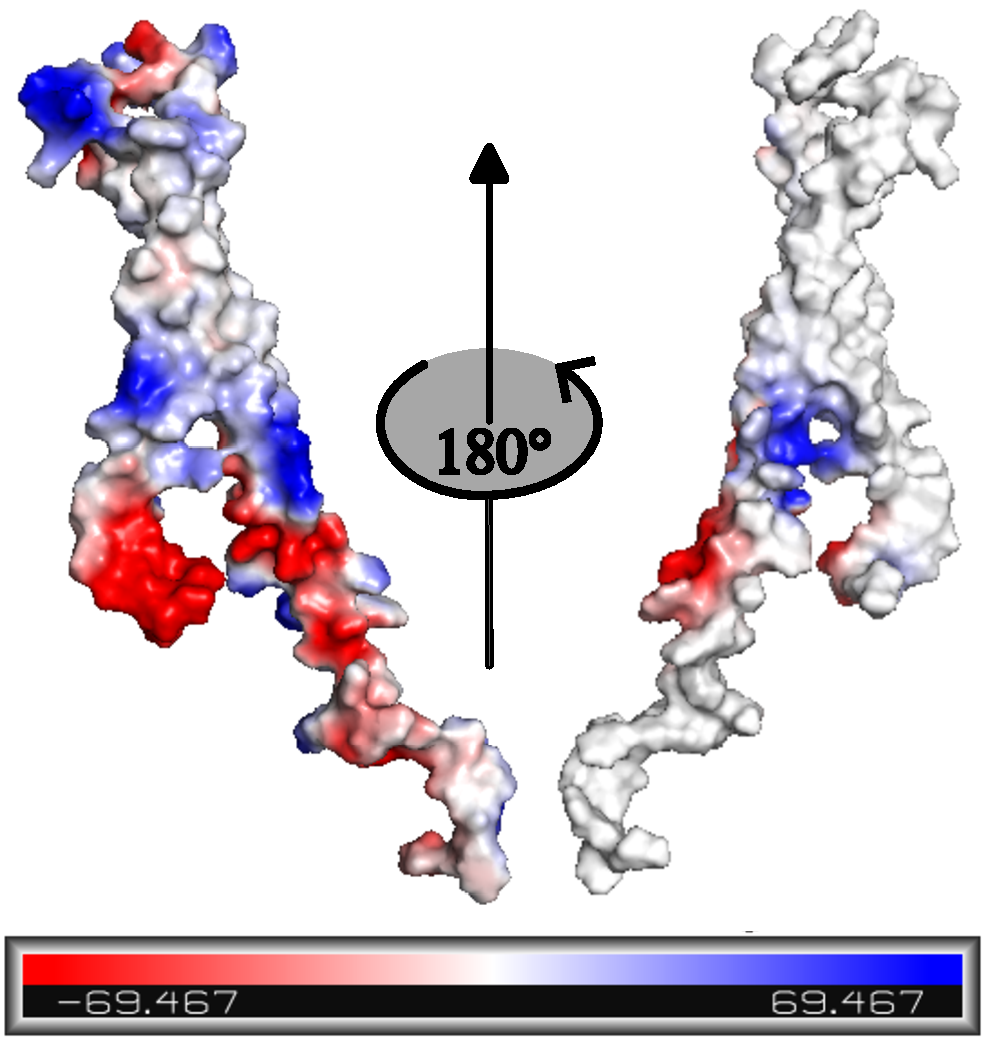
\includegraphics[width=0.79\linewidth]{fig/01_expe/charge_map.pdf}
	\caption[Densidad de carga péptidos]{Densidad de carga péptidos. Los colores corresponden a, \textcolor{red}{rojo: regiones con densidad de carga negativa} y \textcolor{blue}{azul: regiones con densidad de carga positiva}.}
        \index{carga_pept}
    \label{fig:carga_pept}
\end{figure}
%%%%%%%%%%%%%%%%%%%%% Fin %%%%%%%%%%%%%%%%%%%%%%%%

\section{Expresión y purificación de péptidos transmembrana}

La expresión de proteínas por la vía recombinante se ha expandido ampliamente en los últimos años por su versatilidad. Mayoritariamente la obtención de proteínas recombinantes se realiza en células procariotas y la más usada es la bacteria \ac{ecoli} \hl{REF}. El proceso consiste en transformar las bacterias con el plásmido (también conocido como vector) que contiene toda la información genética para expresar la proteína de interés. En este proyecto ambos péptidos se obtuvieron por expresión recombinante empleando bactrias \ac{ecoli} de la cepa BL21(DE3), inducible por \ac{iptg} \hl{REF}. El plásmido empleado para transformar las bacterias fue el pMAL-c2 (ver detalle en la sección \ref{sec:expre_akta}).
Una vez purificada la proteína soluble, que llamamos anteriorme ``proteína fusión'', se clivó con la proteasa \ac{tev} obteniendo la secuencia de los péptidos de interés y posteriorme se repurificaron por \ac{hplc}. 


La \textbf{figura} \ref{fig:expr_hplc_masas}A muestra el seguimiento de la purificación del péptido $\alpha$IIb por \ac{sds}. En los  carriles 1 y 2 se sembró la proteína fusión antes y después del clivaje respectivamente. La pequeña diferencia de peso molecular de $\Xapprox$ 7 kDa, es debida a la ausencia del péptido. En el carril 2 se observa además una banda extra a los $\Xapprox$ 28 kDa que se atribuye a la proteasa \ac{tev}. La banda esperada al péptido no se observa debido a la poca masa que representa. El carril 3 corresponde al pico observado en la cromatografía por \ac{hplc} (\textbf{figura} \ref{fig:expr_hplc_masas}B) que sale en los primeros 6 minutos y se atribuyó a la \ac{mbp}. La banda de peso aparente de $\Xapprox$ 12 kDa en los carriles 4 (fracción directa el HPLC) y 6 (muestra después de retirar \ac{tfa}) corresponden al péptido $\alpha$IIb que corre como dímero debido a su alta hidrofobicidad \hl{REF paper del 2001}. Una vez retirado el \ac{tfa} de las muestras, se realizó un espectro \ac{ftir} en el sistema de \ac{atr} verificando la estructura hélice $\alpha$ mayoritariamente en ambos péptidos, \textbf{figura} \ref{fig:expr_hplc_masas}\textbf{C}. Finalmente la masa molecular de cada péptido fue nuevamente confirmada por espectrometría de masas, resultados que se muestran en la \textbf{figura} \ref{fig:expr_hplc_masas}D-E.

%%%%%%%%%%%%%%%%%%%%% Fig puereza por gel y masas %%%%%%%%%%%%%%%%%%%%%%%%
\begin{figure}[H] % supposedly places it here ...
    \centering
	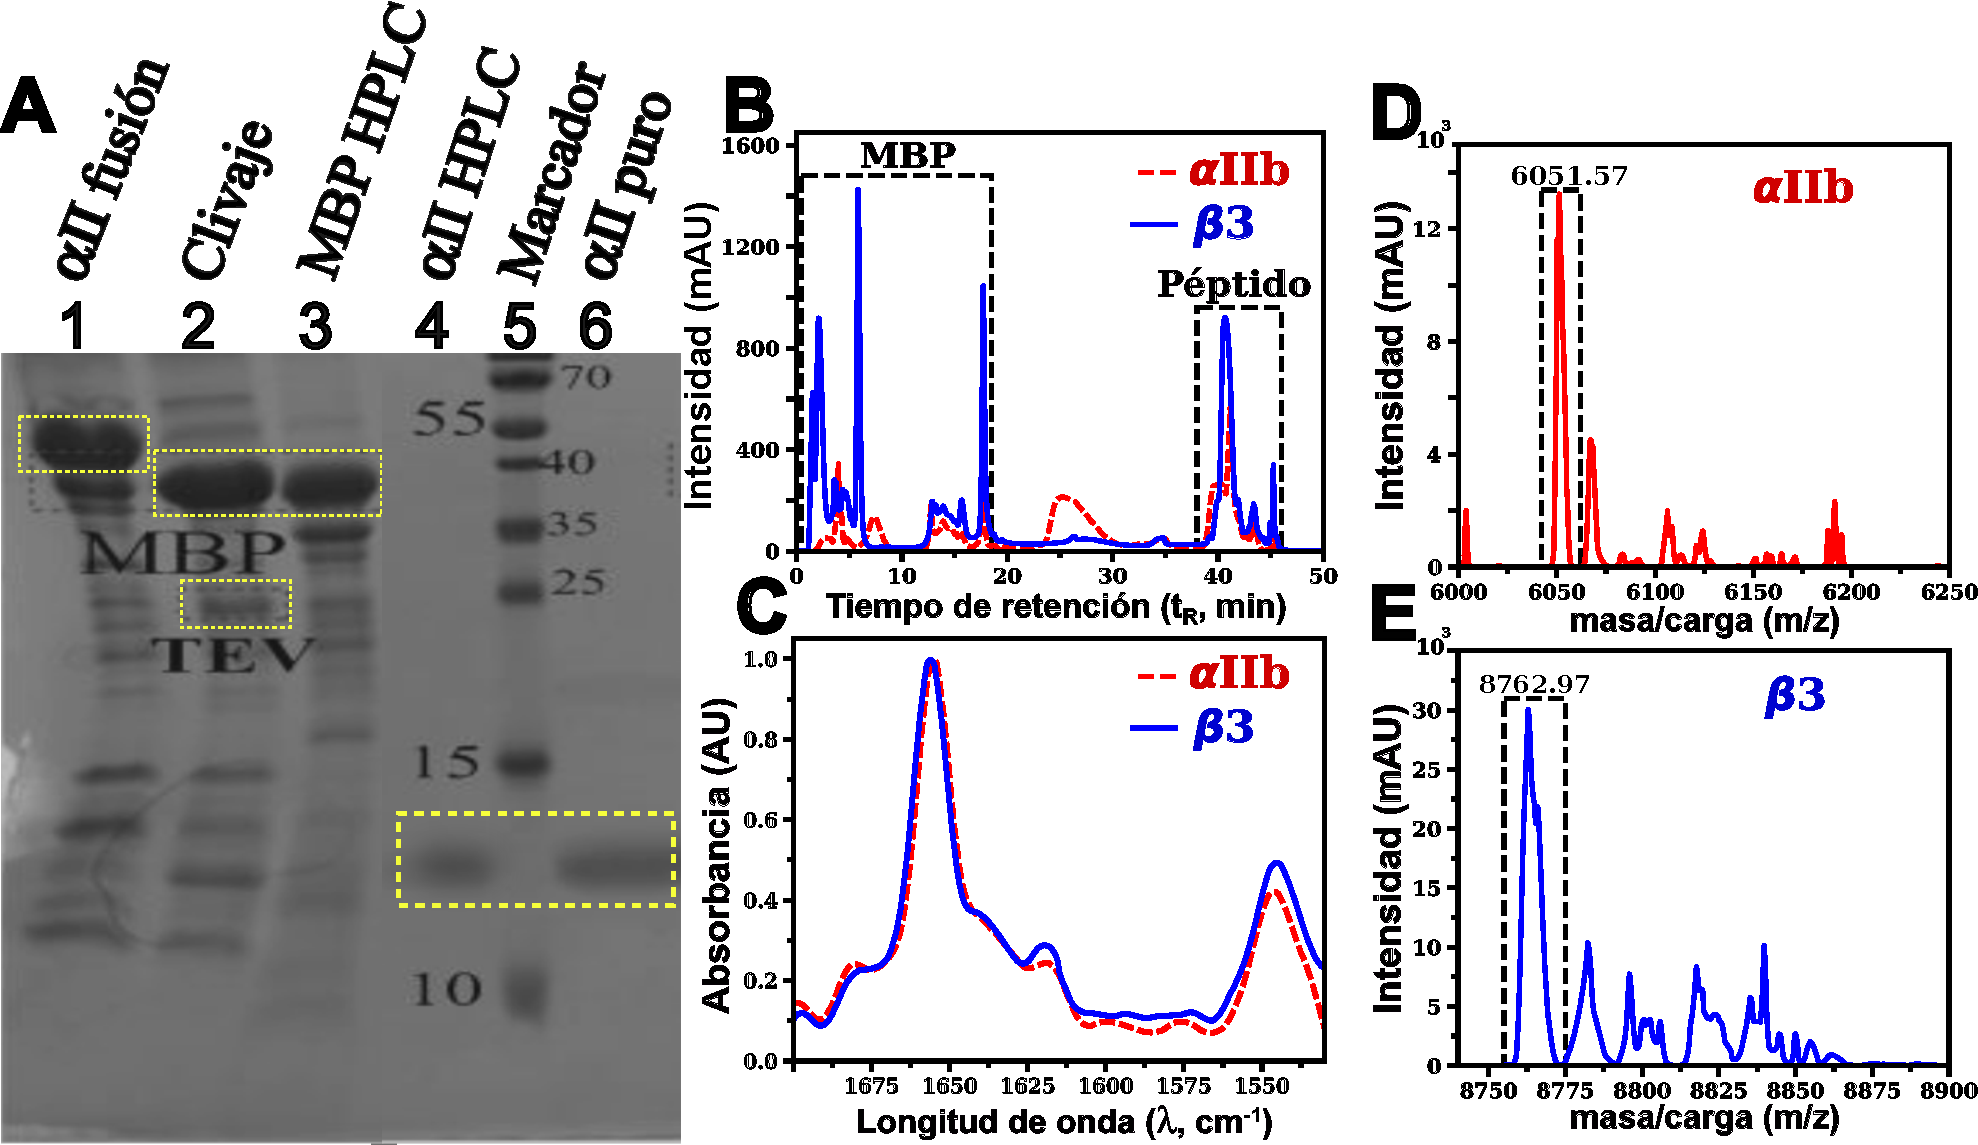
\includegraphics[width=0.99\linewidth]{fig/01_expe/purifi/expres_hplc_masas.pdf}
	\caption[Purificación de péptidos $\alpha$IIb y $\beta$3.]{Purificación de péptidos $\alpha$IIb y $\beta$3. \textbf{A)} Seguimiento de purifición de $\alpha$IIb  por geles \ac{sds}. \textbf{B)} Cromatograma por \ac{hplc} de los péptidos. \textbf{C)} Espectro FT-IR banda de proteína para los dos péptidos y \textbf{D-E)} Espectro de masas para verificación de masa molecular para $\alpha$IIb y $\beta$3 respectivamente.}
        \index{sturcuture_prot}
    \label{fig:expr_hplc_masas}
\end{figure}
%%%%%%%%%%%%%%%%%%%%% Fin %%%%%%%%%%%%%%%%%%%%%%%%





\begin{center} % Center the TikZ picture
\begin{tikzpicture}

% Define box and box title style
\tikzstyle{mybox} = [draw=myblue, fill=blue!10, very thick,
    rectangle, rounded corners, inner sep=10pt, inner ysep=20pt]
\tikzstyle{fancytitle} =[fill=myblue!80, text=white]
\node [mybox] (box){%  
    \begin{minipage}{0.95\textwidth}
    
Las membranas biológicas son un ensamble complejo de una gran variedad de lípidos y proteínas que conjuntamente realizar procesos biológicos importantes a nivel celular. Con la finalidad de entender la funcionalidad de la memebrana, resulta conveniente estudiar las proteínas que son intrínsecamente de membrana. La purificación de proteínas de membrana son un área considerablemente desafiante en la biología molecular \hl{REF}. Un criterio esencial en la purificación de proteínas integrales de membrana es que la proteína debe ser removida cuidadosamente de su ambiente nativo (altamente hidrofóbico) y aislada individualmente en solución. Este solo es posible realizando una secuencia de pasos específicos desde el momento de expresión o síntesis química, de tal forma que en cada paso se recupere la mayor cantidad de la proteína de interés hasta la solubilización con solventes 

%\cite{Carpenter2008}T
%%\cite{Carpenter2008,Eshaghi2009,Matthies2022} \hl{REF}. 

Particularmente en el grupo de investigación del Dr. Guillermo Montich, fue la primera vez que se trabajó con proteínas transmembrana, tampoco había experiencia en el Departamento donde se realizó esta tesis, de otros grupos que hayan expresado y purificado este tipo de proteínas, por lo tanto, una buena parte del tiempo empleado para desarrolar esta tesis consistió en encontrar las condiciones óptimas para la expresión y repurificación los segmentos \ac{tm} de integrimas $\alpha$IIb y $\beta$3. Incluso a modo de anécdota, después de varios intentos sin obtener los péptidos consultamos en laboratorios internacionales que venden el servicio de purificación de proteínas pero después de intercambiar información sobre los péptidos a producir, la respuesta fue que era algo muy complicado y que podría tomar mucho tiempo, buscamos hasta encontrar un laboratorio que tomó el trabajo pero después de dos intentos fallidos nos devolvieron la plata. Queda claro que las proteínas de membrana son desafientes para trabajar, y en el laboratorio hemos desarrollado un protocolo para la obtención de  los segmentos \ac{tm}-\ac{ic} de $\alpha$IIb y $\beta$3 que puede utilizarse para producir estos péptidos y posiblemente péptidos similares. Además, algo que poco se ha mensionado, fue que también se produjo por expresión recombinante la proteasa \ac{tev} que es de venta comercial.

    \end{minipage}
};
\node[fancytitle, right=10pt] at (box.north west) {\Large{Purificación proteínas transmembrana}};
\node[fancytitle, rounded corners] at (box.east) {\faComment };
\end{tikzpicture}%
\end{center}
\chapter{Interacción lípido-péptido en monocapas de Langmuir}\label{mono}


\section{Monocapas de Langmuir}
Las monocapas de Langmuir  han sido ampliamente usadas como modelo de biomembrana para estudiar las interacciones lípido-proteína en interfases agua-aire \hl{REF}. La formación de monocapas de lípidos y proteínas está favorecida termodinámicamente debido a que disminuyen la tensión superficial del agua. Considerando que la energía libre de superficie, $\gamma$, representa el cambio de energía libre de Gibbs del sistema cuando las moléculas particionan a la interfase con el cambio de área, \textit{A}, a temperatura y presión constante \hl{REF}.

\begin{equation}\label{ecu:gamma}
   \gamma =  \left(\frac{\partial G}{\partial A}\right)_{T,P}
\end{equation}

Se define la presión lateral superficial, $\pi$ (ecuación \ref{ecu:pi}) donde $\gamma_0$ y $\gamma$ son la tensión superficial de la subfase pura y de la muestra, respectivamente.


\begin{equation}\label{ecu:pi}
    \pi =  \large{\gamma_0} \;  \text{--} \;  \large{\gamma}
\end{equation}

Podemos obtener información sobre la estructura e interacciones de las moléculas en la interfase midiendo la presión lateral en función del área ocupada por la monocapa. El experimento consiste en depositar lentamente sobre la subfase acuosa gotas de una solución de anfifílos (lípidos, péptidos, proteínas o sus mezclas) en solventes de alta presión de vapor. Al evaporarse el solvente queda una capa monomolecular de soluto en la interfase. En las isotermas de compresión medimos la presión lateral en función del área ($\pi$--\textit{A}) de interfase utilizando una balanza de Wilhelmy \hl{REF}. 

\subsection{Transiciones de fase en monocapas}

En las isotermas $\pi$--\textit{A} se observan regiones característica que corresponden
a diferentes estados de organización molecular, también llamados estados de fase. Las diferentes fases son el resultados de rearreglos moleculares. Cuando la película se encuentra totalmente expandida, es decir, en condiciones de $\pi$ $\Xapprox$ 0.0 mN/m, la distancia entre moléculas vecinas es mucho más grande que el tamaño de cada molécula, y este se describe como un estado gaseoso (G) en dos dimenciones. Al comprimir la monocapa disminuyendo el área, las moléculas se reorganizan pasando a un estado más compactado conocido como \ac{le}. Al continuar la compresión se lleva al siguiente estado de fase conocido como \ac{lc}, donde las moléculas presentan un estado más compacto y menos compresible. En este estado las moléculas se orientan perpendicularmente a la interfase con  los grupos polares interactuando preferentemente con el agua y los grupos apolares dirigidos hacia el aire. El próximo estado, y anterior al colapso, es el estado sólido (S), con alto grado de compactación y baja compresibilidad. Finalmente, una posterior disminución del área lleva al colapso de la monocapa, donde los valores $\pi$ empiezan a fluctuar arbitrariamente debido a la formación de multicapas, o desorción de las moléculas hacia la fase acuosa. También podemos identificar zonas con coexistencia de fases:  G--\ac{le} y el \ac{le}--\ac{lc} \hl{REF}.

Las isotermas $\pi$--\textit{A}  permiten obtener información acerca de la estructura, área, compresibilidad, histéresis, transición de fase, cambios conformacionales e interacciones entre sus componentes. En este trabajo se utilizaron monocapas de Langmuir para evaluar la estabilidad interfacial de los segmentos \ac{tm}-\ac{ic} de los péptidos $\alpha$IIb y $\beta$3 puros, una vez caracterizadas sus propiedades individuales, se estudiaron las interaciones que establecen con \ac{popc}, \ac{dppc} y la mezcla \ac{popc}:\ac{popg} 70:30, que llamaremos \textbf{PCPG}.

\section{Monocapas de péptidos puros}\label{mono_pept_puros}

Antes de realizar los experimentos de moncapas de Langnuir de los péptidos puros, surge la pregunta ¿cómo se espera que se orienten los péptidos en la interfase agua-aire?. En las proteínas nativas, ambos péptidos tienen estructura hélice $\alpha$. Si consideramos a un péptido transmembrana como un cilindro (\textbf{figura} ~\ref{fig:orientTM}B), podemos inferir acerca de su orientación a partir de las medidas de área molecular en capas monomoleculares. Un área molecular experimental similar al área del cilindro indicaría un arreglo de péptidos orientados perpendicularmente a la interfase y altamente compactados como se representa en la \textbf{figura} ~\ref{fig:orientTM}A-\textit{ii}. Para ambos péptidos, a partir de las estructuras publicadas \cite{Yang2009}, usando la librería MDAnalysis \hl{REF} y considerando sólo el segmento con estructura hélice $\alpha$ definida, evaluamos un radio promedio de 12.1 Å (área de 460 Å\textsuperscript{2}). Esta es el área por molécula que deberíamos observar a la presión de colapso si los péptidos se empaquetaran perpendicularmente a la interfase y en estructura hélice $\alpha$. Valores mayores de área molecular corresponderían a otras orientaciones no perpendiculares o en estados conformacionales expandidos, desordenados y no correspondientes con hélice $\alpha$.
%%RAdio calculado en la notebook de dppc "Radio alfa hélice"

%%%%%%%%%%%%%%%%%%%%% Fig {Modelo de posible orientación %%%%%%%%%%%%%%%%%%%%%%%%
\begin{figure}[H] % supposedly places it here ...
    \centering
	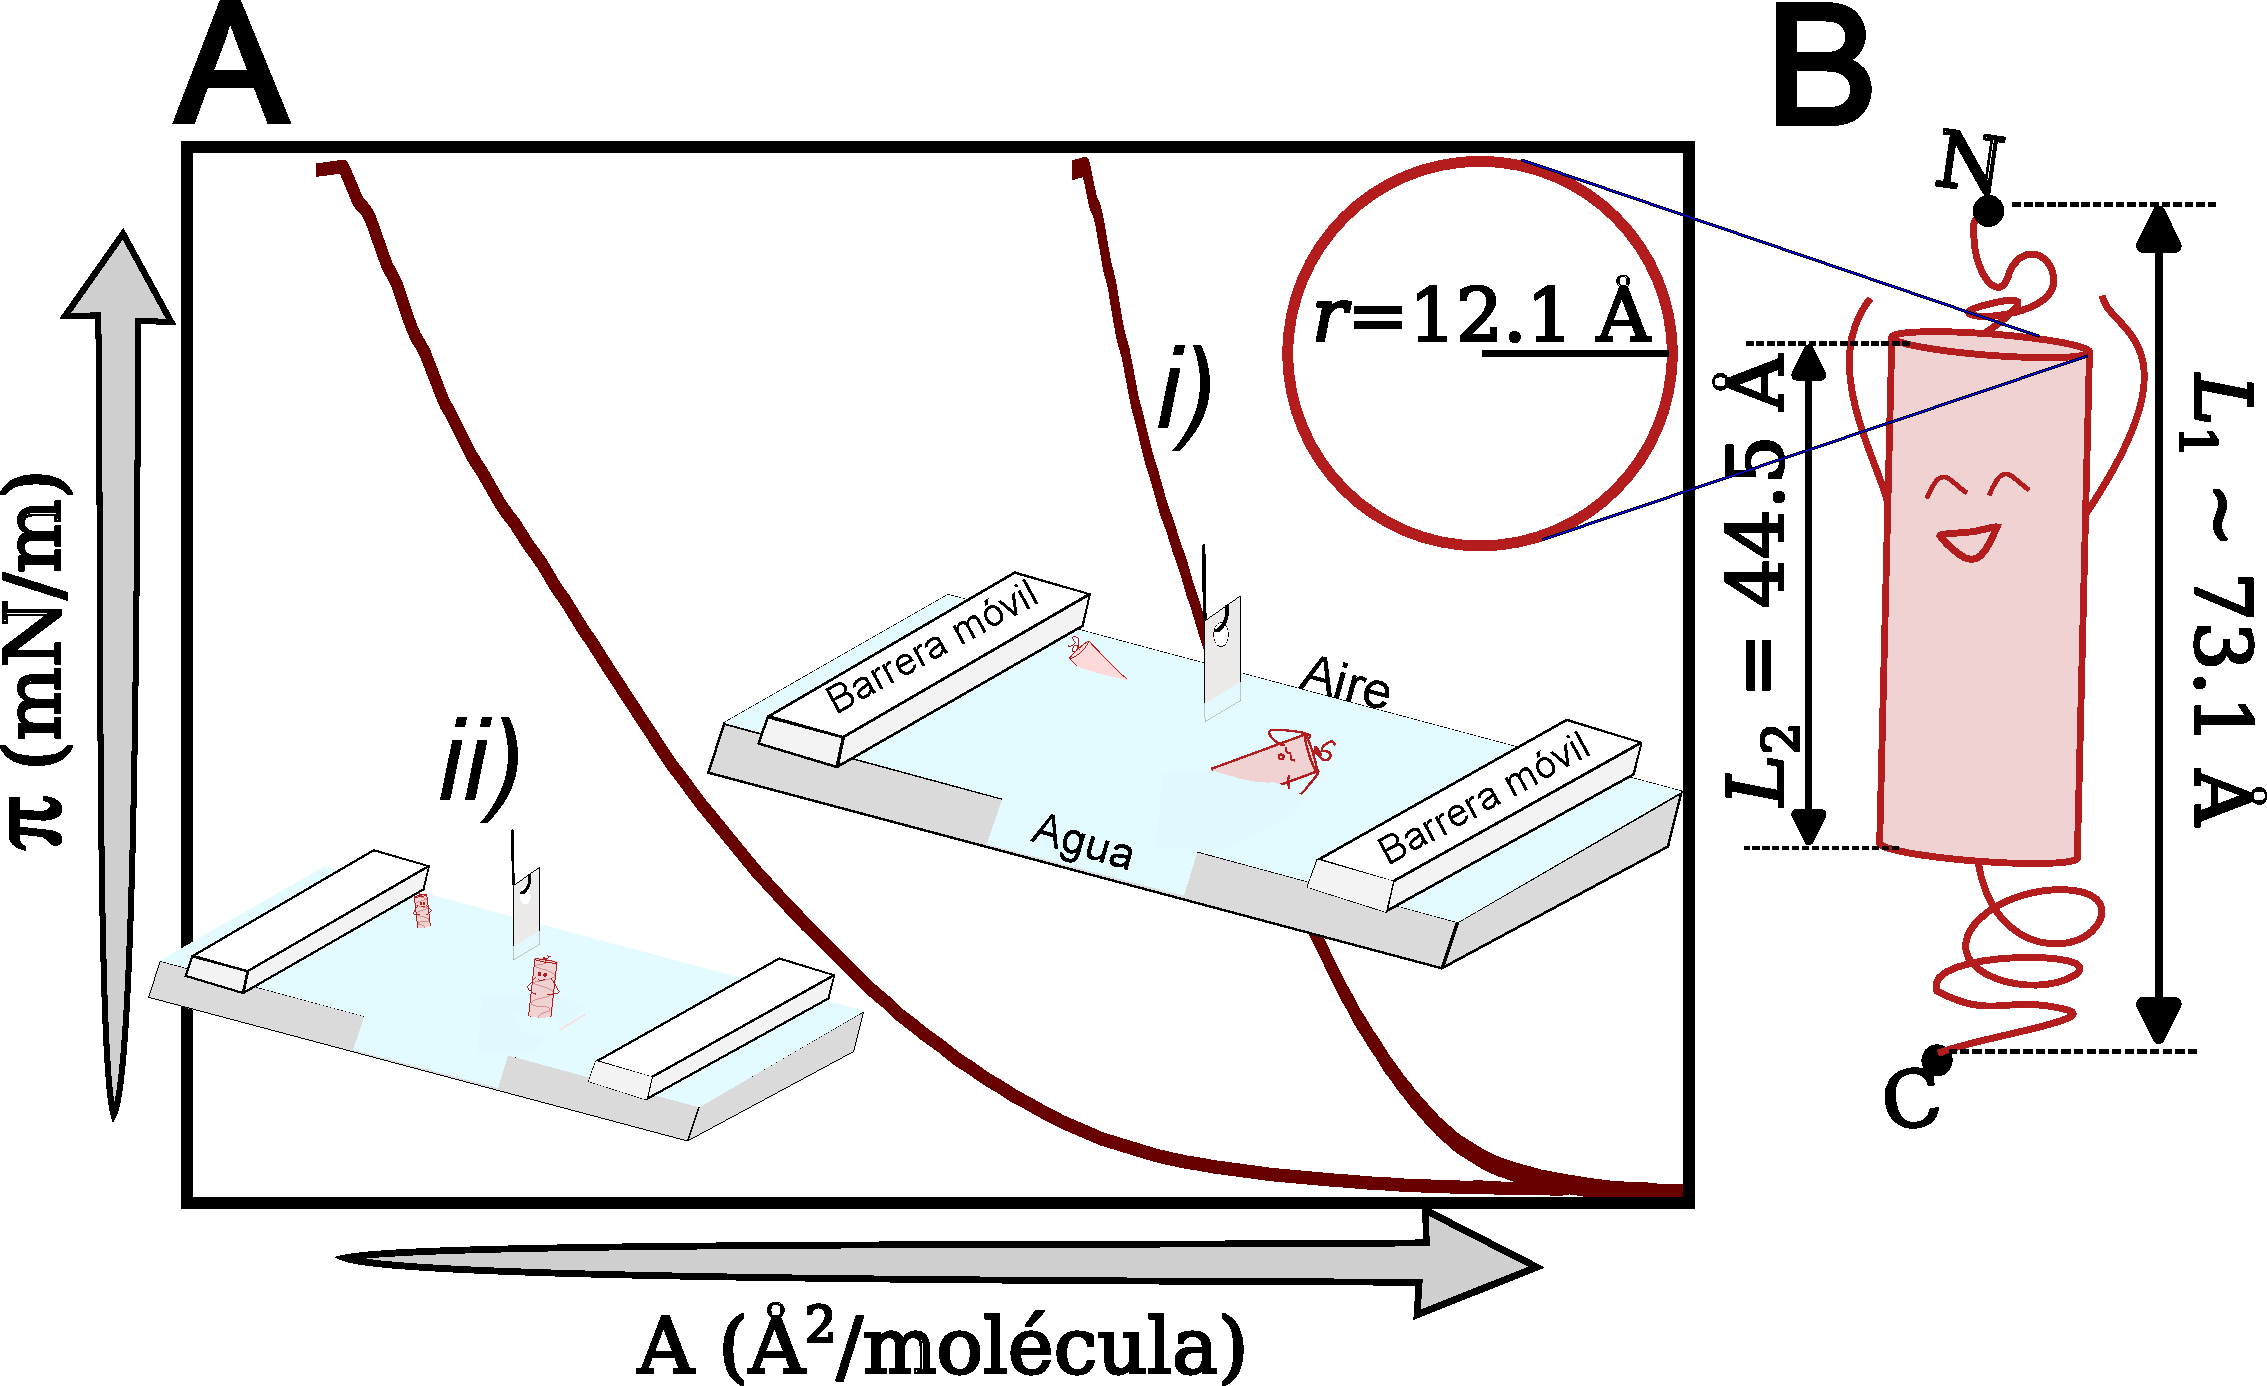
\includegraphics[width=0.85\linewidth]{fig/01_expe/orienta_pept2.pdf}
	\caption[Modelo de posible orientación de $\alpha$-hélice en el plano de una monocapa.]{Modelo de posible orientación de hélice $\alpha$ en el plano de una monocapa.}
        \index{orientacion}
    \label{fig:orientTM}
\end{figure}
%%%%%%%%%%%%%%%%%%%%% Fin %%%%%%%%%%%%%%%%%%%%%%%%


Ambos péptidos presentan actividad superficial en monocapas de Langmuir (\textbf{figura}~\ref{fig:area_pi_pept}A). Forman monocapas estables que pueden ser comprimidas en al menos dos ciclos de compresión-descompresión sin perder material por partición a la subfase. La siembra de 0.5 nmoles no produjo un aumento de presión significativamente diferente de cero y corresponde a un área de $\Xapprox 2500$ Å\textsuperscript{2}/molécula. A 5 mN/m, los péptidos se han compactado y el área molecular es de  $\Xapprox 1300$ Å\textsuperscript{2}. A presiones de  35 y 42 mN/m para $\alpha$IIb y $\beta$3, el área molecular fue de $\Xapprox 482$ \textpm 52 y $\Xapprox 593$ \textpm 20 Å\textsuperscript{2} para $\alpha$IIb y $\beta$3 respectivamente. Estos valores de área molecular indican que los péptidos tiene un radio de 12.4 Å para $\alpha$IIb y 13.7 Å para $\beta$3, y tienden a organizarse perpendicularmente al plano de la monocapa en estructura hélice $\alpha$ tal como se sugirió en la \textbf{figura} ~\ref{fig:orientTM}A-\textit{ii}. Algunos autores \cite{Barlow1988, Kato2015,Ionov2000,Weder2003} han reportado un radio promedio de 5.0 Å en hélices $\alpha$ el cual da un área de  78.5 Å\textsuperscript{2} y más reciente Mura et al. \cite{Mura2013} reportó un radio de 10 Å valor que correspondería un área molecular de 314.6 Å\textsuperscript{2}. Las áreas para los dos péptidos se encuentran cercanos a éste último valor. Por último nos preguntamos, cuál es la orientación de los péptidos, es decir, ¿\textit{del N- al C-terminal ó del C- al N-terminal}?. El no colapso de la monocapa estaría dado por las posibles fluctuaciones de la región que no tiene estructura secundaria definida (segmento \ac{ic}), por tanto a presiones bajas estas regiones son las que se localizan preferentemente en la subfase mientras que las  hélice $\alpha$, región hidrofóbica, se orienta hacia el aire. A medida que se comprime la monocapa, las colas forman ``loops'' que aumentan de tamaño y pueden oscilar a medida que se compacta y por lo tanto no se llega a una presión de colapso (ver \textbf{figura} \ref{fig:mono_pept}, flechas \textcolor{blue}{\faLongArrowRight}), algo similar reportaron Toimil et al. \cite{Toimil2012} para álbumina sérica humana. A un presión 35 mN/m el péptido $\alpha$IIb presentó un áréa molecular ligeramente mayor al esperado teóricamente (460 Å\textsuperscript{2}), éste valor se calculó teniendo en cuenta sólo la región con estrucutura secundaria hélice $\alpha$, de igual forma con $\beta$3. El área experimental de $\beta$3 es más grande comparado con $\alpha$IIb, y puede ser porque $\beta$3 tiene un dominio citoplasmático más largo no estructurado. \\

%%%%%%%%%%%%%%%%%%%%%Fig. Isotermas de compresión peptidos %%%%%%%%%%%%%%%%%%%%%

\begin{figure}[h!] % supposedly places it here ...
    \centering
	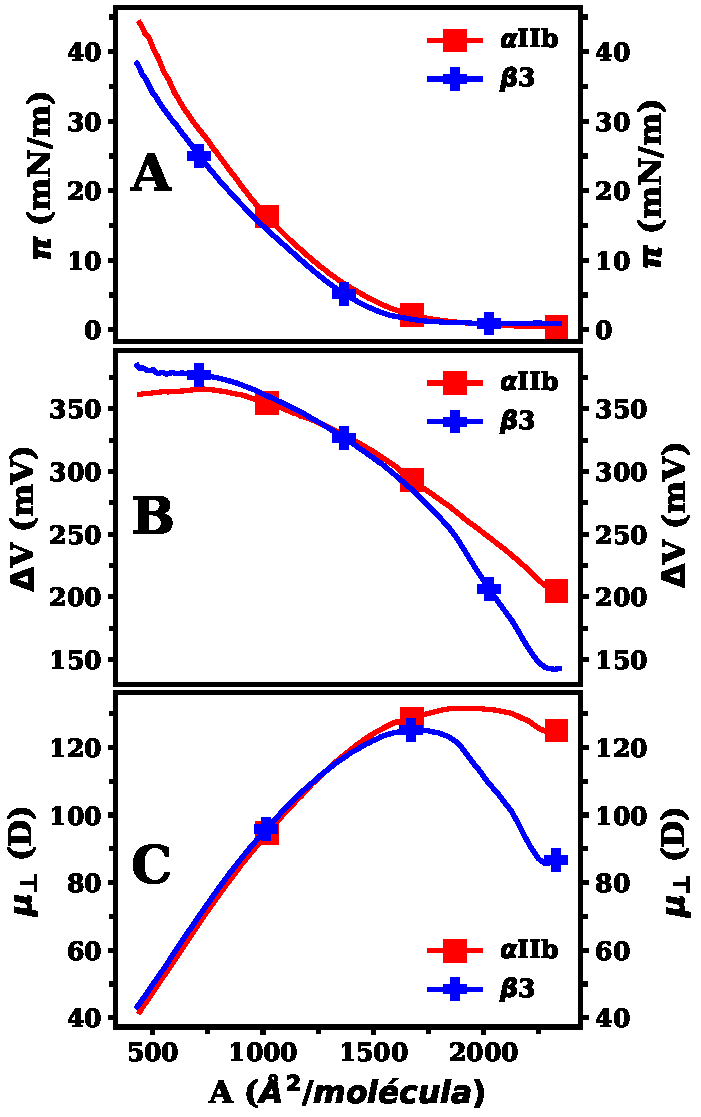
\includegraphics[width=0.5\linewidth]{fig/01_expe/mono/area_pi_peptidos.pdf}
	\caption[Isotermas de compresión en la interfase agua/aire para péptidos puros.]{Isotermas de compresión en la interfase agua/aire para péptidos puros. \textbf{A)} Presión superficial ($\pi$), \textbf{B)} potencial de superficie $\Delta V$ y  \textbf{C)} momento dipolar total, respecto al área molecular media (\textbf{A)}}.
        \index{area_pi_pept}
    \label{fig:area_pi_pept}
\end{figure}
%%%%%%%%%%%%%%%%%%%%% Fin %%%%%%%%%%%%%%%%%%%%%%%%

Helmholtz propone que en una monocapa las especies químicas que estan cerca de la superficie del agua presentan una orientación específica \hl{REF}. Ésta orientación viene dada por los dipolos de cada especie y puede describirse por la siguiente ecuación,

\begin{equation}
    \label{ecu:potencial}
    \Delta V =  \frac{12 \Pi \mu_\perp}{A}
\end{equation}

Donde $\Delta V$ es el potencial de superficie (mV) medido entre el seno de la solución acuosa y la \hl{fase gaseosa (aire)}, \textit{A} el área molecular (Å\textsuperscript{2}), $\Pi$ es constante  y $\mu_\perp$ el momento dipolar total de superficie ($\mu_\perp$). El $\Delta V$, medido en una monocapa tiene tres contribuciones: 1) los dipolos ordenados de las moléculas adsorbidas, 2) los dipolos de las moléculas de agua ordenadas en la zona de la superficie, 3) el dipolo generado por la doble capa iónica de Gouy-Chapman  en en caso que las moléculas adsorbidas tengnan cargas netas \cite{Brockman1994,Electronics1994}. Se observó que aún cuando la presión de superficie es indistinguible de cero, el $\Delta V$ es significativamente grande y alcanza valores de entre 200 y 150 mV para $\alpha$IIb y $\beta$3 respectivamente (\textbf{figura} \ref{fig:area_pi_pept}B). 
%%%$\mu_\perp$ = $\mu_1$ + $\mu_2$ + $\mu_3$, $\mu_1$ es la contribución de las moléculas de agua orientadas al rededor de las caras hidrofílicas de la proteína, $\mu_2$ y $\mu_3$ contribuciones hidrofílica e hidrofóbica de la proteína que esta en contacto con la superficie 
En los dos péptidos el $\mu_\perp$ inicia con valores relativamente altos (\textbf{figura} ~\ref{fig:area_pi_pept}C) y a medida que se comprime lateralmente va dismuniyendo hasta alcanzar los $\Xapprox 43$ D al valor mínimo área molecular, esta tendencia abre la posibilidad a realizar el siguiente planteamiento de reorganización, inicialmente los péptidos se encuentran con una supercie de contacto mayor expuesta al agua y por lo tanto, hay alta densidad de carga que contribuye al $\mu_\perp$  (\textbf{figura} \ref{fig:mono_pept}A-B-C, sin embargo al compactarse lateralmente, los péptidos tienen a orientarse verticalmente, exponiendo menos residuos al superficie de la monocapa, disminuyendo la densidad de cargar, finalmente se llega a un estado donde estan lo sufientemente  compactactados que todo lo que tiene estructura $\alpha$ hélice queda expuesto al aire y la única parte que contribuye al $\Delta$V y/o $\mu_\perp$ es la región que fluctúa de estrucutra y que tiene mayor caracter polar; un planteamiento similar realizó Maget \cite{Maget-Dana1999}.

%%%% \textbf{figura} modelo compactacion pept en monocapas%%%
\begin{figure}[H] 
    \centering
	
\includegraphics[width=0.99\linewidth]{fig/01_expe/mono_pept.pdf}
	\caption{Modelo de reorganización de los péptidos en monocapas de Langmuir y fluctuación de estrucuta secundaria en segmento intracelular para los péptidos $\alpha$IIb y  $\beta$3.}
        \index{mono_pept}
    \label{fig:mono_pept}
\end{figure}
%%%%%%%%%%%%%%%%%%%%% Fin %%%%%%%%%%%%%%%%%%%%%%%%} 

Para tener una mejor idea de lo planteado anteriormente acerca de cómo se orientan los péptidos la monocapa de Langmuir, se realizó un análisis de la hidrofobicidad promedio por residuo <H> \, y del momento hidrofóbico $\mu_H$ para cada péptido (ver \textbf{tabla} ~\ref{tab:mu_hidrofo}). En los dos péptidos, el domino \ac{tm} presenta mayor <H> \,  respecto a los dominios \ac{ec} e \ac{ic}, principalmente dado por la cantidad de residuos hidrofóbicos (\textbf{figura} ~\ref{fig:mu_hidrofo}, resaltados en amarillo \begin{tikzpicture}
  \node[draw, circle, fill=yellow, line width=0.5pt, inner sep=1pt, scale=0.6, font=\color{yellow}] {\faCircle}; \end{tikzpicture}). El <H> \, del dominio \ac{ec} es más grande (0.693\textgreater\!\textgreater -0.091) que dominio \ac{ic} del péptido $\alpha$IIb, además, el domino \ac{ic} presenta cuatro cargas negativas comparadas a una carga positiva del dominio \ac{ec}. El péptido $\beta$3 tiene 25 residuos más que $\alpha$IIb en el dominio \ac{ic} (\textbf{figura} ~\ref{fig:mu_hidrofo}, ``\textbf{55-79}''), éstos últimos residuos que a aportan un caracter hidrofóbico aunque sigue siendo menor comparado al dominio \ac{ec} (0.163\textless\!\textless 0.360), además, también hay la presencia de una carga positiva. Por tanto en los dos péptidos, es más probable que el dominio \ac{ic} interactúe con la fase acuosa, lo cual conduce a plantear que los péptidos se orientan del \textit{del N- al C-terminal}.


%%%%Tabla resumen de H_mu%%%%
\begin{table}[H]
%\begin{wraptable}{r}{0.50\textwidth}
%\vspace{-0.7cm} 
\centering
\begin{threeparttable}
\centering
\caption{Resumen hidrofobicidad y carga para los dominios \ac{ec}, \ac{tm} y \ac{ic} de péptidos $\alpha$IIb y  $\beta$3.}\label{tab:mu_hidrofo}
\begin{tabular}{@{}llccl@{}}
\toprule
Péptido     & N° Residuo             & <H>      	& <$\mu_H$> 	& z  \\ \midrule
$\alpha$IIb & \multirow{2}{*}{1-11 \; (EC) }  & 0.185  	& 0.273 		& 1- \\
$\beta$3    &                        & 0.360  	& 0.341 		& 0  \vspace{3mm} \\
$\alpha$IIb & \multirow{2}{*}{12-36 \;(TM)} & 1.182  	& 0.133 		& 1+ \\
$\beta$3    &                        & 1.183  	& 0.121 		& 1+ \vspace{3mm} \\
$\alpha$IIb & \multirow{2}{*}{37-54 \;(IC)} & -0.091 	& 0.263 		& 4- \\
$\beta$3    &                        & -0.091 	& 0.184 		& 0  \vspace{3mm} \\
$\beta$3    & 55-79 \;(IC)                  & 0.163  	& 0.233 		& 1+ \\ \bottomrule
\scriptsize{\ac{ec}: \acl{ec}} & \scriptsize{\ac{tm}: \acl{tm}} & \scriptsize{\ac{ic}: \acl{ic}}
\end{tabular}
\end{threeparttable}
%\vspace{-0.5cm} 
%\end{wraptable}
\end{table}
%%%%%Fin tabla%%%%%



\hl{Es importante destacar que la evaluación de la actividad superficial comprende la integración de múltiples factores contribuyentes, entre ellos la anfipaticidad, el tamaño molecular, la flexibilidad estructural, la carga neta y las interacciones intramoleculares. Esta complejidad inherente en la composición y el comportamiento de las moléculas subraya las dificultades inherentes en la medición precisa del potencial de superficie. Además, es relevante reconocer que, dadas estas variadas influencias, los resultados experimentales relativos a esta propiedad suelen exhibir una considerable variabilidad, manifestándose en una dispersión significativa en comparación con los valores teóricos anticipados. Esta observación resalta la necesidad de un enfoque meticuloso y detallado en la interpretación de los datos experimentales, considerando la gama de variables que pueden afectar las mediciones del potencial de superficie..}\\

\begin{figure}[H] % supposedly places it here ...
    \centering
	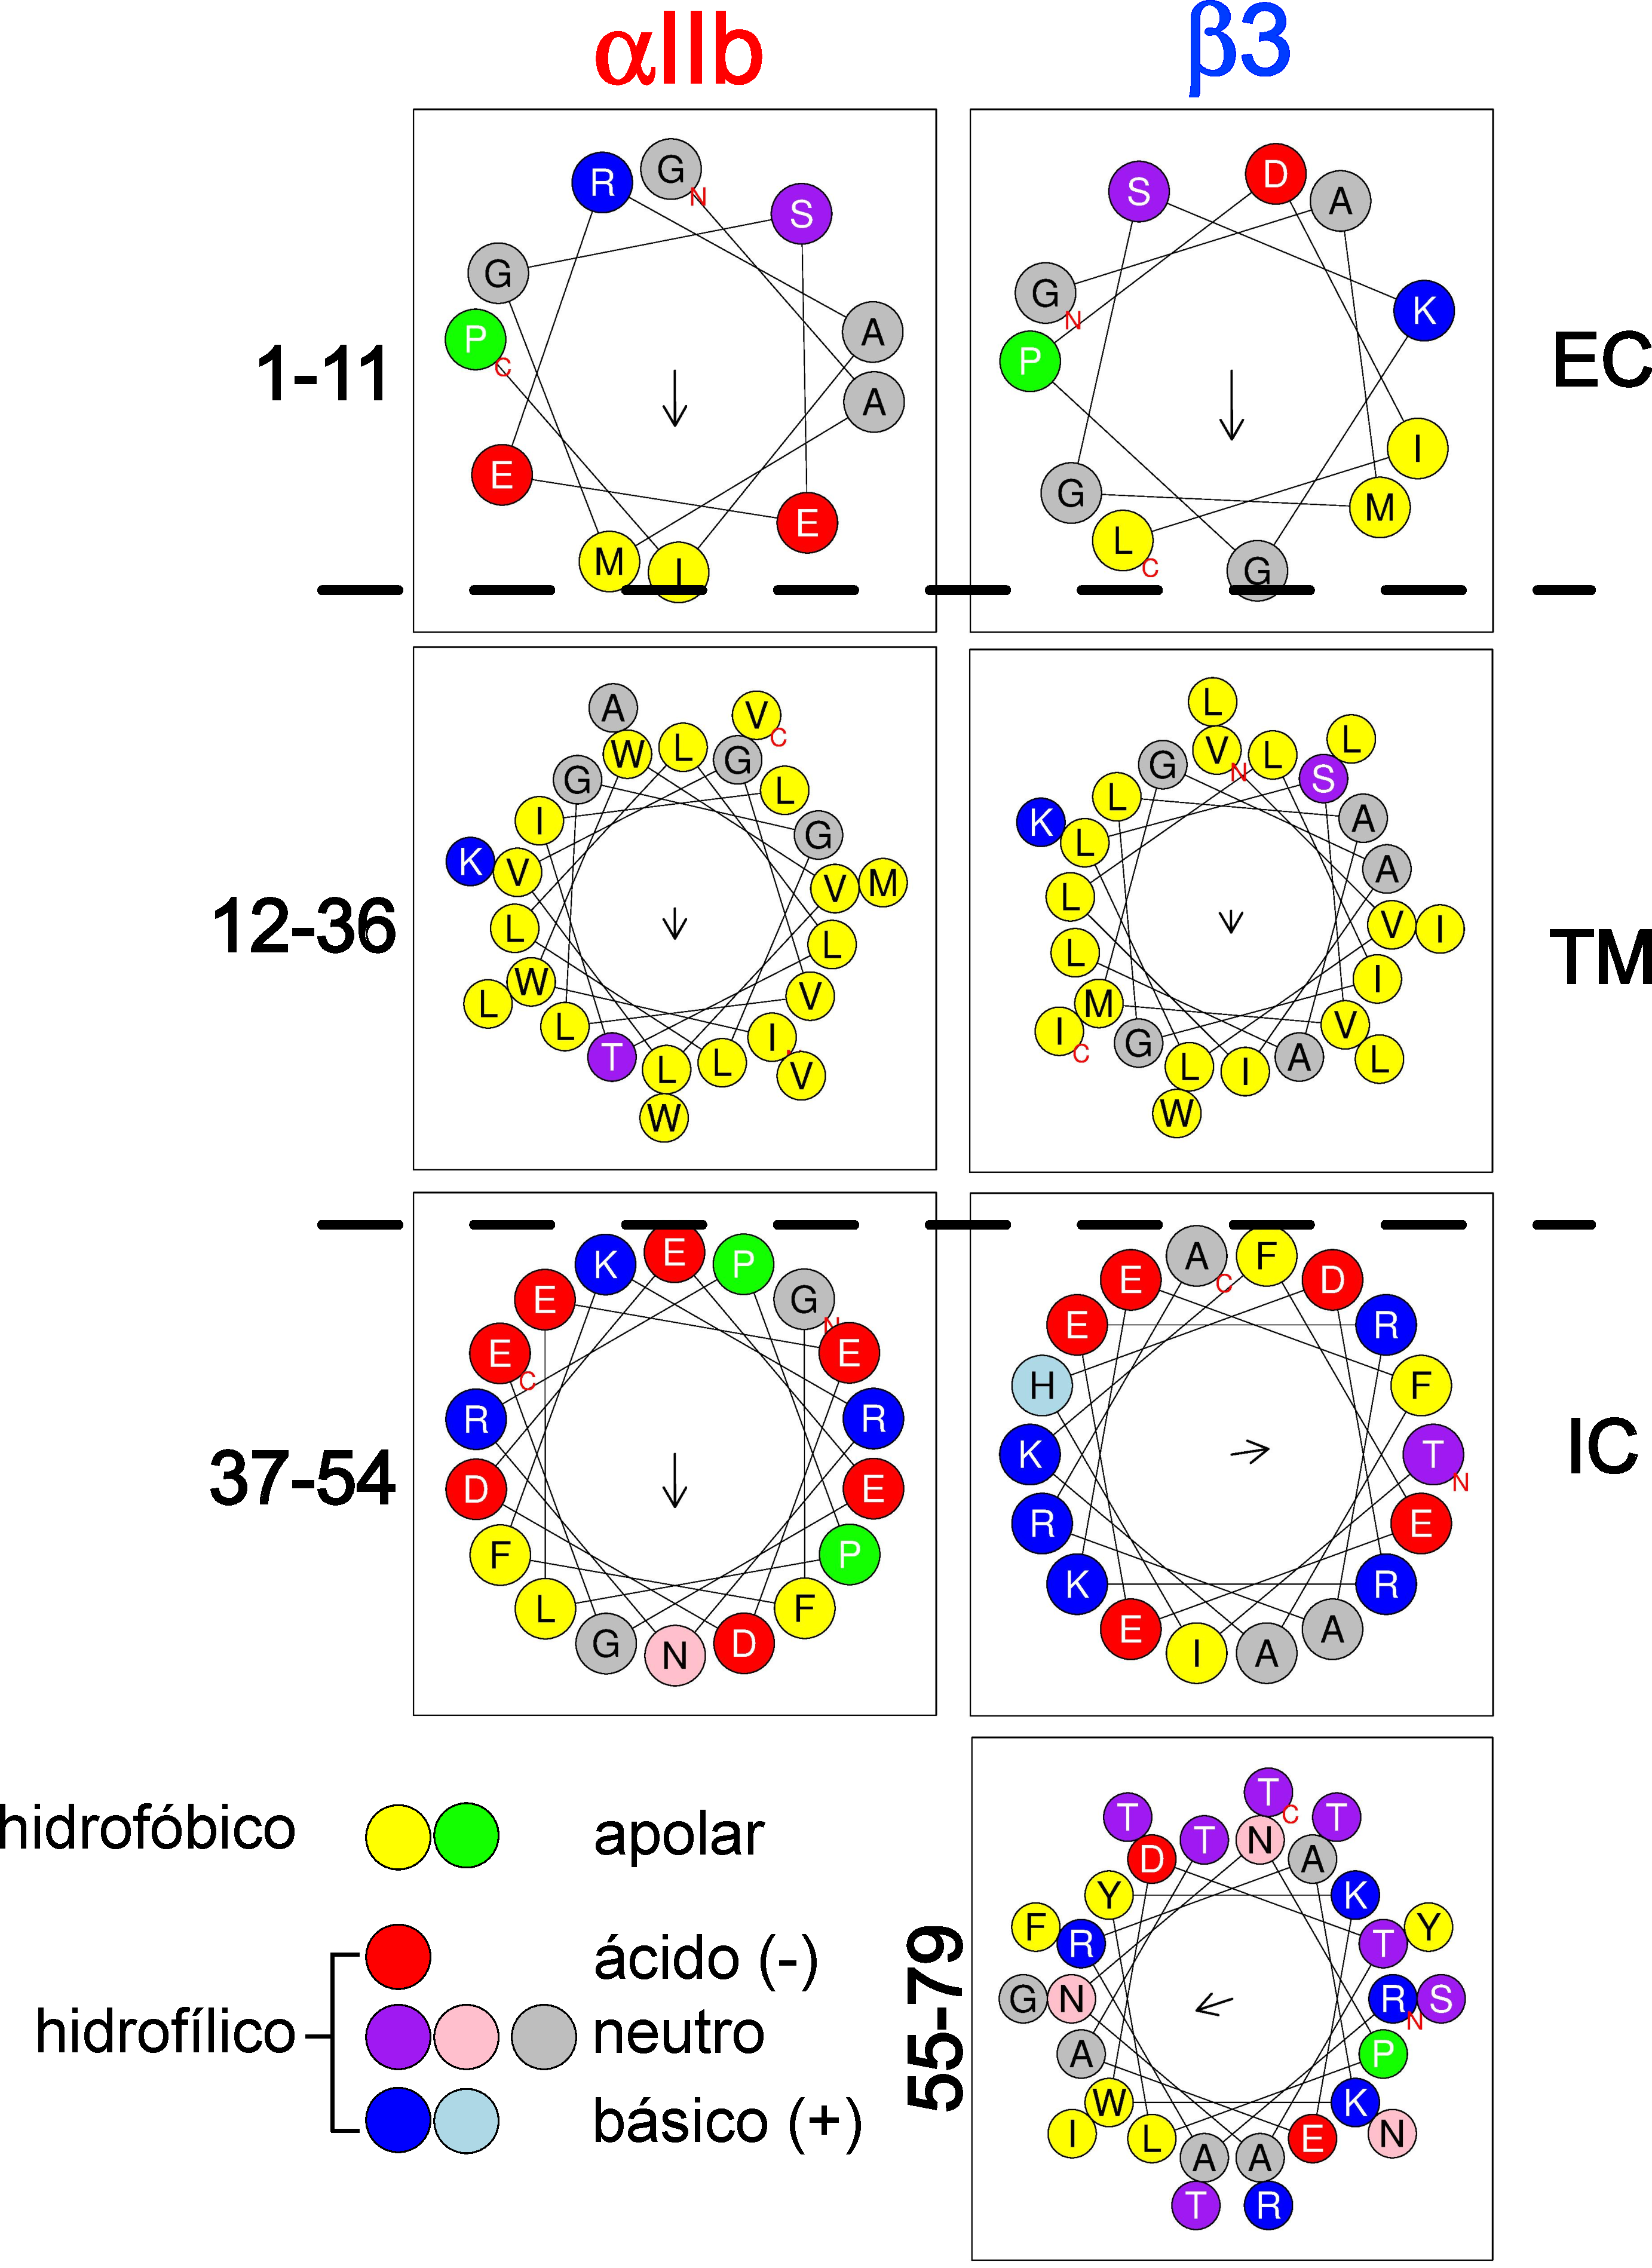
\includegraphics[width=0.7\linewidth]{fig/01_expe/secuencias_alfa_beta.pdf}
	\caption[Proyección circular de la hélice para las secuencias de los segmentos transmembrana $\alpha$IIb y  $\beta$3.]{Proyección circular de la hélice para las secuencias de los segmentos transmembrana $\alpha$IIb y  $\beta$3. La fecha (\textrightarrow) en el centro indica la magnitud y la dirección del momento hidrofóbico <$\mu_H$>. La proyección se realizó con el software HeliQuest  (\url{https://heliquest.ipmc.cnrs.fr}).}
        \index{mu_hidrofo}
    \label{fig:mu_hidrofo}
\end{figure}
%%%%%%%%%%%%%%%%%%%%% Fin %%%%%%%%%%%%%%%%%%%%%%%%

\section{Monocapas de Langmuir para mezclas lípido-péptido}\label{sect:mono_mezclas}

Se realizaron isotermas de compresión de lípido puro (\ac{popc}, PCPG, \ac{dppc}) y mezclas lípido-péptido ($\alpha$IIb ó $\beta$3) en concentraciones de crecientes de péptido desde 0.0 a 7.0\% mol. En la \textbf{figura} ~\ref{fig:area_pi_all}, panel superior de  se muestran las mezclas de lípido-$\alpha$II y en el inferior las mezclas lípido-$\beta$3. En todos los experimentos se realizaron 3 ciclos de compresión-expansión para evaluar la estabilidad del film lípido-péptido. Para la mezcla \ac{popc}/$\alpha$IIb se observó que en todos los casos se produjo un corrimiento a áreas mayores respecto al lípído puro y este pareciera ser mayor con el incremento de la concentración de péptido. En PCPG/$\alpha$IIb se observó que hay el lípido tiene a compactarse o por lo menos a estar más cerca de la isoterma de la mezcla pura PCPG; y para la mezcla \ac{dppc}/$\alpha$IIb el efecto de expansión fue más notorio en los tres sistemas estudiados, incluso en todas la concentraciones se observó que la pretransición en \ac{dppc} no se percibe ya con 2.0\% de péptido (\textcolor{emerald}{\rotatebox{0}{\faStar}}). Respecto a las mezclas en presencia de $\beta$3, presentaron compartamientos similares a lo observado con el péptido $\alpha$IIb, en la mezcla con PCPG el corrimiento a areas menores es más marcado en concentraciones de 2.0\% y 3.5\% (\textcolor{falured}{\rotatebox{90}{\faPlay}}).
Comparando un poco más en detalle el efecto de los dos péptidos,  en las monocapas de \ac{popc}, a 5.0\% (\textcolor{goldenpoppy}{\faCircle}) de $\alpha$IIb se desplaza a áreas menores comparado las concentraciones más bajas que iba aumentando pero luego a 7.0\% (\textcolor{deepmagenta}{$\pentagonblack$}) se recupera dicha tendencia, mientras que en presencia de $\beta$3 sucede el mismo efecto pero a 2.0\% y luego se produce el corrimiento a áreas mayores. Para la mezlca binaria de lípidos PCPG, pareciera que a bajas concentraciones de péptido 2.0\% y 3.5\% se produce en efecto de compactación, siendo más notorio cuando se trata de $\beta$3. En presencia de \ac{dppc} el corrimiento hacia áreas mayores al incrementar la concentración de péptido se cumple para ambos péptidos, sin embargo, en presencia de $\beta$3 esa tendencia se sigue hasta 5.0\% porque luego a 7.0\% baja a corrimientos similares al 2.0\% de $\beta$3.

%%%%%%%%%%%%%%%%%%%%%Fig. Isotermas de compresión %%%%%%%%%%%%%%%%%%%%%
\begin{figure}[H] % supposedly places it here ...
    \centering
	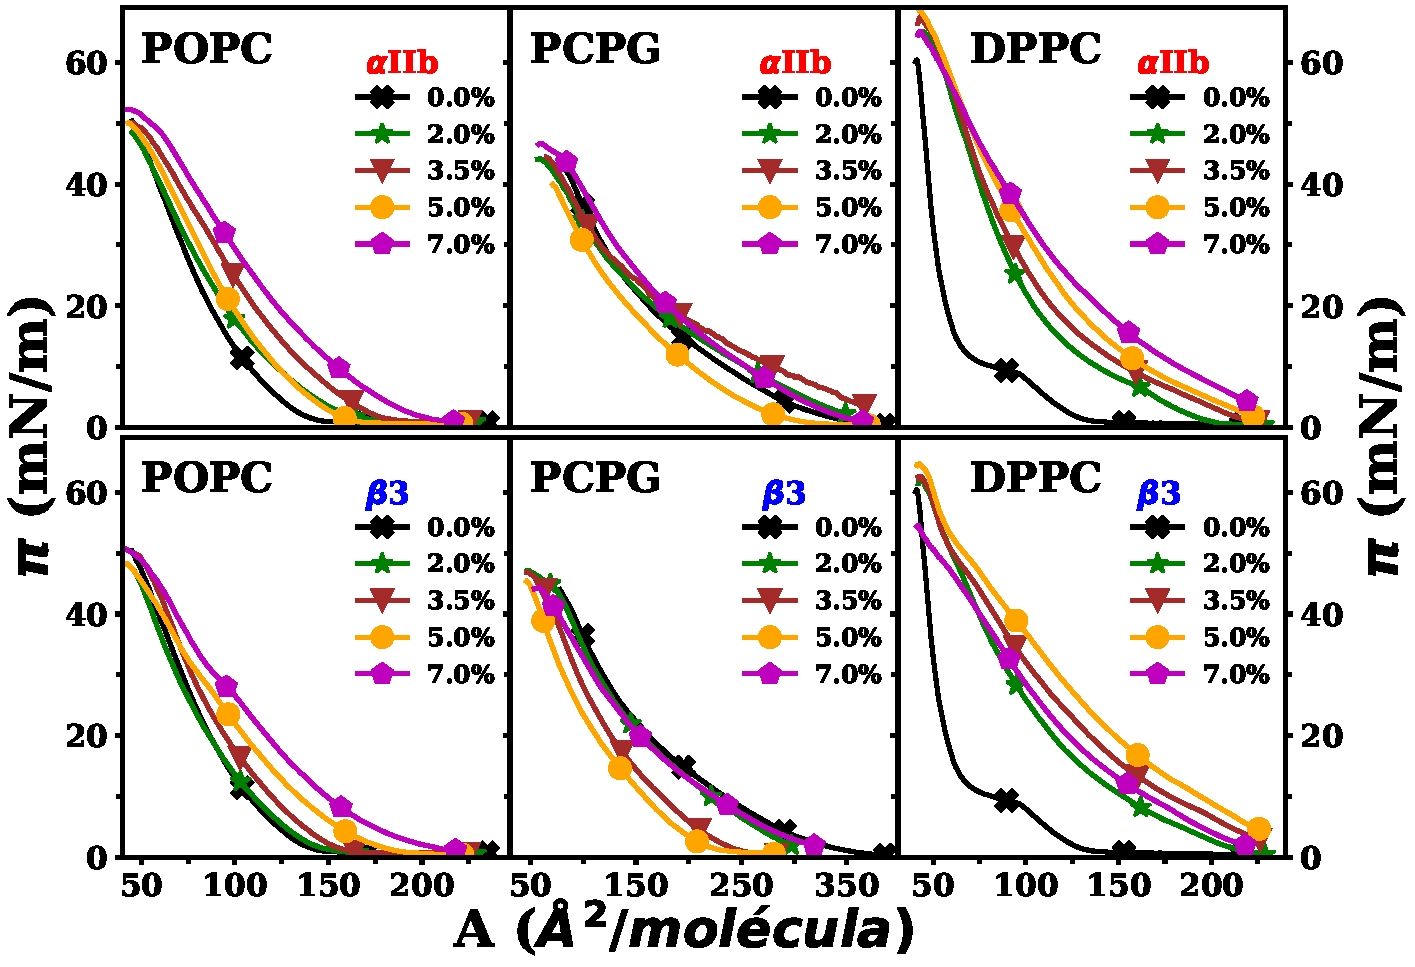
\includegraphics[width=0.99\linewidth]{fig/01_expe/mono/area_pi_all.pdf}
\caption[Isotermas de compresión, presión superficial -- área molecular promedio (\boldmath{$\pi$}--A) en la interfase aire-agua.]{Isotermas de compresión, presión superficial -- área molecular promedio (\boldmath{$\pi$}--A) en la interfase aire-agua de los sistemas lípido-péptido (lípidos = POPC, POPC:POPG  70:30 llamdao PCPG y  DPPC). Panel superir lípdio/$\alpha$IIb, panel inferior lípido/$\beta$3; las concentraciones crecientes de péptido están idicadas en cada sub\textbf{figura} por marcadores respectivos.}
        \index{area_pi_all}
    \label{fig:area_pi_all}
\end{figure}
%%%%%%%%%%%%%%%%%%%%% Fin %%%%%%%%%%%%%%%%%%%%%%%%

%Dado que de los gráficos anteriores no se puede realizar conclusiones generales de cómo interactúan los péptidos con los lípidos, se procedió a realizar un análisis del área molecular promedio vs el porcentaje de péptido a diferentes presiones con la finalidad de encontrar alguna tendencia más evidente para cada sistema estudiado (ver la siguiete sección  ~\ref{AvsMol}).


%%%%%%%%%% Àrea Vs %mol
\section{Análisis de la miscibilidad  de mezclas lípido-péptido}{\label{AvsMol}}

Como previamente se observó las monocapas monomoleculares permiten evaluar las característi de empaquetamiento molecular, además también es posible obtener una idea de cómo es el grado de miscibilidad lípido-péptido comparando el área molecular promedio de la mezcla a una dada presión superficial (propiedad aditiva). El área de una mezcla es comparada con las área media moleculares de cada componente por separado a una dada presión superficial. Las áreas de las mezclas ideales $A_{ideal}$ para dos componentes fue calculada según la ecuación ~\ref{ecua:Aideal} \citep{Ali1994} a las presiones de 2 y 30 mN/m,

\begin{equation}
    \label{ecua:Aideal}
    A_{ideal} = \left[X_{\text{L}}A_{\text{L}} + X_{\text{P}}A_{\text{P}}\right]_\pi
\end{equation}

Donde $A_{L,P}$ son las áreas moleculares promedio y $X_{L,P}$ son las fracciones molares del lípido y péptido respectivamente a una determinada presión. Los componentes de la mezcla tendrán un área $A_{ideal}$ si estos no interaccionan, o lo hacen hacen idealmente, por lo tanto cualquier desviación de la idealidad es atribuída a interacciones específicas que pueden ser atractivas (el área observada es menor al $A_{ideal}$) o repulsivas (el área observada es mayores al $A_{ideal}$) entre los componentes. 
A partir de los datos de la \textbf{figura} ~\ref{fig:area_pi_all} se calcularon las áreas $A_{ideal}$  para cada mezcla a las presiones mencionadas y se compararon  respecto a los datos experimentales.
A una presión superficial de 2 mN/m (\textbf{figura} ~\ref{fig:Fig_AreaVsMoles}--panel superior), las áreas moleculares promedio observadas sugieren que ambos péptidos presentan interacciones atractivas lípido-péptido en los sistemas \ac{popc} y PCPG, mientras que en la mezcla \ac{dppc}-péptido el comportamiento es de caracter repulsivo a concentraciones de 2.0\% a 5.0\%.
En el panel inferior (\textbf{figura} ~\ref{fig:Fig_AreaVsMoles}) se muestra el mismo análisis a 30 mN/m y la tendencia de los datos experimentales es similar a los observado a 2 mN/m en para todas las mezclas lípido-péptido. 

%%%Tabla con carácterísticas de los lípidos
\begin{table}[H]
\centering
\begin{threeparttable}
\centering
\caption[Generalidades lípidos]{Generalidades lípidos}\label{tab:lipidos}
%\begin{wraptable}{r}{0.52\textwidth}
%\vspace{-0.8cm} %%%Posiciona a una altura en la hoja
\begin{tabular}{lccc}
\hline
Lípido                       & \cellcolor[HTML]{EFEFEF}Enlace & \cellcolor[HTML]{EFEFEF}Fase a 25°C & \cellcolor[HTML]{EFEFEF}Carga neta \\ \hline
\cellcolor[HTML]{CBCEFB}POPC & 16:0-18:1                      & LE                                  & 0   \\
\cellcolor[HTML]{CBCEFB}POPG & 16:0-18:1                      & LE                                  & 1-- \\
\cellcolor[HTML]{CBCEFB}DPPC & 16:0                           & múltiples                           & 0 \\
\hline\\
\end{tabular}
%    \vspace{-1.51cm} %%%espacio entre texto y botton table
%%    \end{wraptable} 
\end{threeparttable}
\end{table}
%%%%%Fin tabla%%%%%


%%%%%%%%%%%%%%%%%%%%%% Fig A Vs %mol %%%%%%%%%%%%%%%%%%%%%%%%
\begin{figure}[h] % supposedly places it here ...
    \centering
	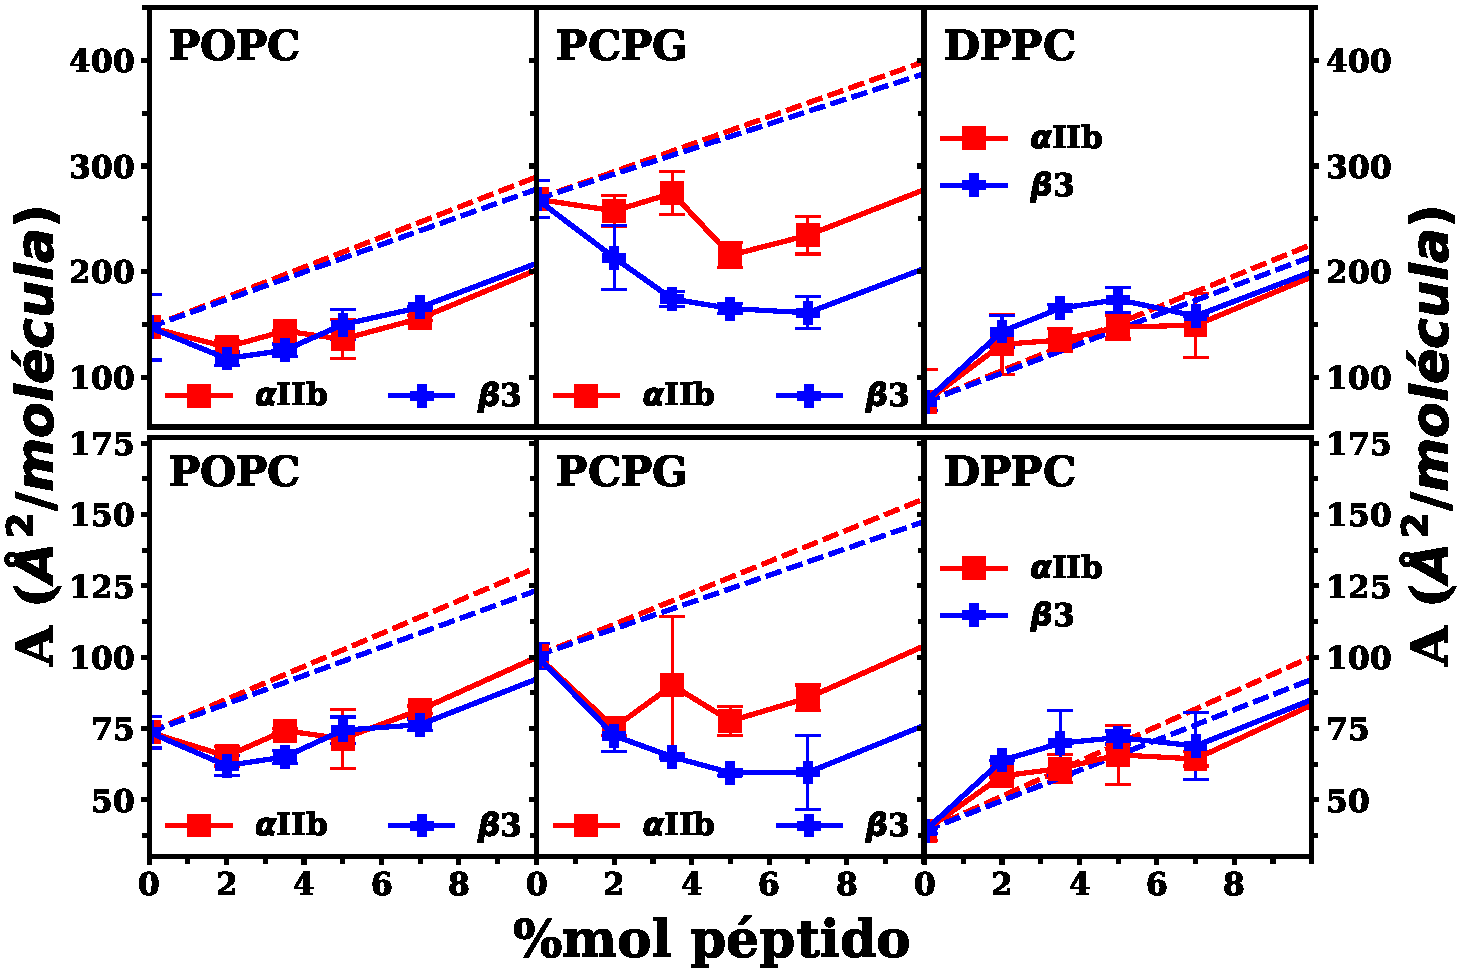
\includegraphics[width=0.99\linewidth]{fig/01_expe/mono/Aideales_all2.pdf}
	\caption[Área molecular promedio Vs porcentaje molar (A--\%mol péptido) para cada sistema lípido-péptido.]{Área molecular promedio Vs porcentaje molar (A--\%mol péptido) para cada sistema lípido-péptido (lípidos = POPC, POPC:POPG  70:30 llamdao PCPG y  DPPC). Panel superior e inferior 2 y 30 mN/m, respectivamente. Las líneas  - - - indican la curva de idealidad para las mezclas.}

     \index{Fig_AreaVsMoles}
    \label{fig:Fig_AreaVsMoles}
\end{figure}
%%%%%%%%%%%%%%%%%%%%% Fin %%%%%%%%%%%%%%%%%%%%%%%%


Para comprender un poco más en detalle lo que podría estar sucediendo a nivel molecular, veamos algunas características de los lípidos en particular. En la \textbf{tabla} \ref{tab:lipidos} vemos que el \ac{popc} y POPG tiene el mismo tipo de enlaces en la cadena hidrofóbica y también el mismo largo de cadena (átomos de carbono) y misma fase a temperatura ambiente (líquido expandido, LE),  con la diferencia el POPG tiene carga neta negatiga mientras que el \ac{popc} es zwiteriónico, por otra parte el \ac{dppc} es un lípido saturado (no posee dobles enlaces), es de 16 carbonos en ambas cadenas hidrofóficas y tiene múltiples transiciones de fase. Con base en estas características, retomando lo observado en la \textbf{figura} ~\ref{fig:Fig_AreaVsMoles} vemos que ambos péptidos tienden a compactar los lípidos con LE e interaccionan de forma repulsiva (expanden) el \ac{dppc} que presenta pricipalmente una fase líquido condensado (LC). También se vio que en la mezcla PCPG que tiene carga negativa, interacciona preferentemente con el péptido $\beta$3 que tiene carga neta de 2+, comparado con el $\alpha$IIb.



%%%%Paper Properties of the Langmuir and Langmuir–Blodgett monolayers
%%%%of cholesterol‑cyclosporine A on water and polymer support
%%%%https://doi.org/10.1007/s10450-019-00117-2

Recientemente los autores Socas, L. y Ambroggio, E. \cite{Socas2018,Socas2023} propusieron un modelo matemático para comparar isotermas de compresión en monocapas. En lugar de comparar las isotermas a presiones definidas, como se realizó anteriormente a 2 y 30 mN/m, el modelo compara cuantitativamente las isotermas en todo el rango de presiones. La comparativa de dos isotermas distintas, designadas respectivamente como la isoterma de interés e isoterma de referencia, implica la instauración de un parámetro denominado factor $\Lambda$ definido por dos parámetros: 

\begin{equation}
    \label{ecua:lambda}
    \Lambda = \left(\lambda,r^2 \right)
\end{equation}

Donde $\lambda$ representa un factor de \textit{distancia} entre las áreas moleculares media de las isotermas y r$^2$ el grado de “similitud” entre la forma de las curvas a lo largo de todo el rango de presiones comunes en ambas isotermas. Primero se determina el rango de valores de presión que son comunes a ambas isotermas  (de referencia y de interés) y se emplea un algoritmo de regresión no lineal para encontrar el  valor de λ que minimice la diferencia de cuadrados entre los valores del área molecular promedio (\textbf{A}) de la isoterma de interés y los calculados para cada valor de presión según:

\begin{equation}
    \label{ecua:lambda2}
    \textbf{A}\text{(} \pi \text{)} = \lambda \; \text{x} \; \textbf{A}_{\text{referencia}} \text{(} \pi \text{)}
\end{equation}

 Finalmente se procede a calcular el coeficiente de determinación (r$^2$), que proporciona una medida cuantitativa de la congruencia entre la curva isoterma resultante y la curva isoterma de interés. Los valores obtenidos para  r$^2$ y $\lambda$ se abordan de la siguiente manera:

%%%%%Tabla de significado lambda%%%%%%%%%%%%
\begin{table}[H]
%\centering
\begin{threeparttable}
\centering
%\caption[Factor $\Lambda$ para comparar cuantitativamente isotermas]{Factor $\Lambda$ para comparar cuantitativamente isotermas}\label{tab:lambda}
\begin{tabular}{lcl}
\rowcolor[HTML]{ECF4FF} 
\multicolumn{1}{r}{\cellcolor[HTML]{ECF4FF}r$^2$ y $\lambda$ = 1} &  & Isotermas idénticas                \\
\rowcolor[HTML]{CBCEFB} 
\cellcolor[HTML]{CBCEFB}                            & $\lambda$ \textgreater{} 1 & Similar en forma con desplazamiento hacia áreas moleculares \textbf{mayores} \\
\rowcolor[HTML]{CBCEFB} 
\multirow{-2}{*}{\cellcolor[HTML]{CBCEFB}r$^2$ $\Xapprox 1$ } & $\lambda$ \textless{} 1 & Similar en forma con desplazamiento hacia áreas moleculares \textbf{menores} \\
\rowcolor[HTML]{ECF4FF} 
r$^2$ \textless{}\textless{} 1                                                           &  & Las isotermas no se parecen en forma
\end{tabular}
\end{threeparttable}
\end{table}
%%%%%Fin tabla%%%%%


%%%%%%%%%%%%%%%%%%%%%% Tabla LAMBDA %%%%%%%%%%%%%%%%%%%%%%%%

\begin{figure}[h] % supposedly places it here ...
    \centering
	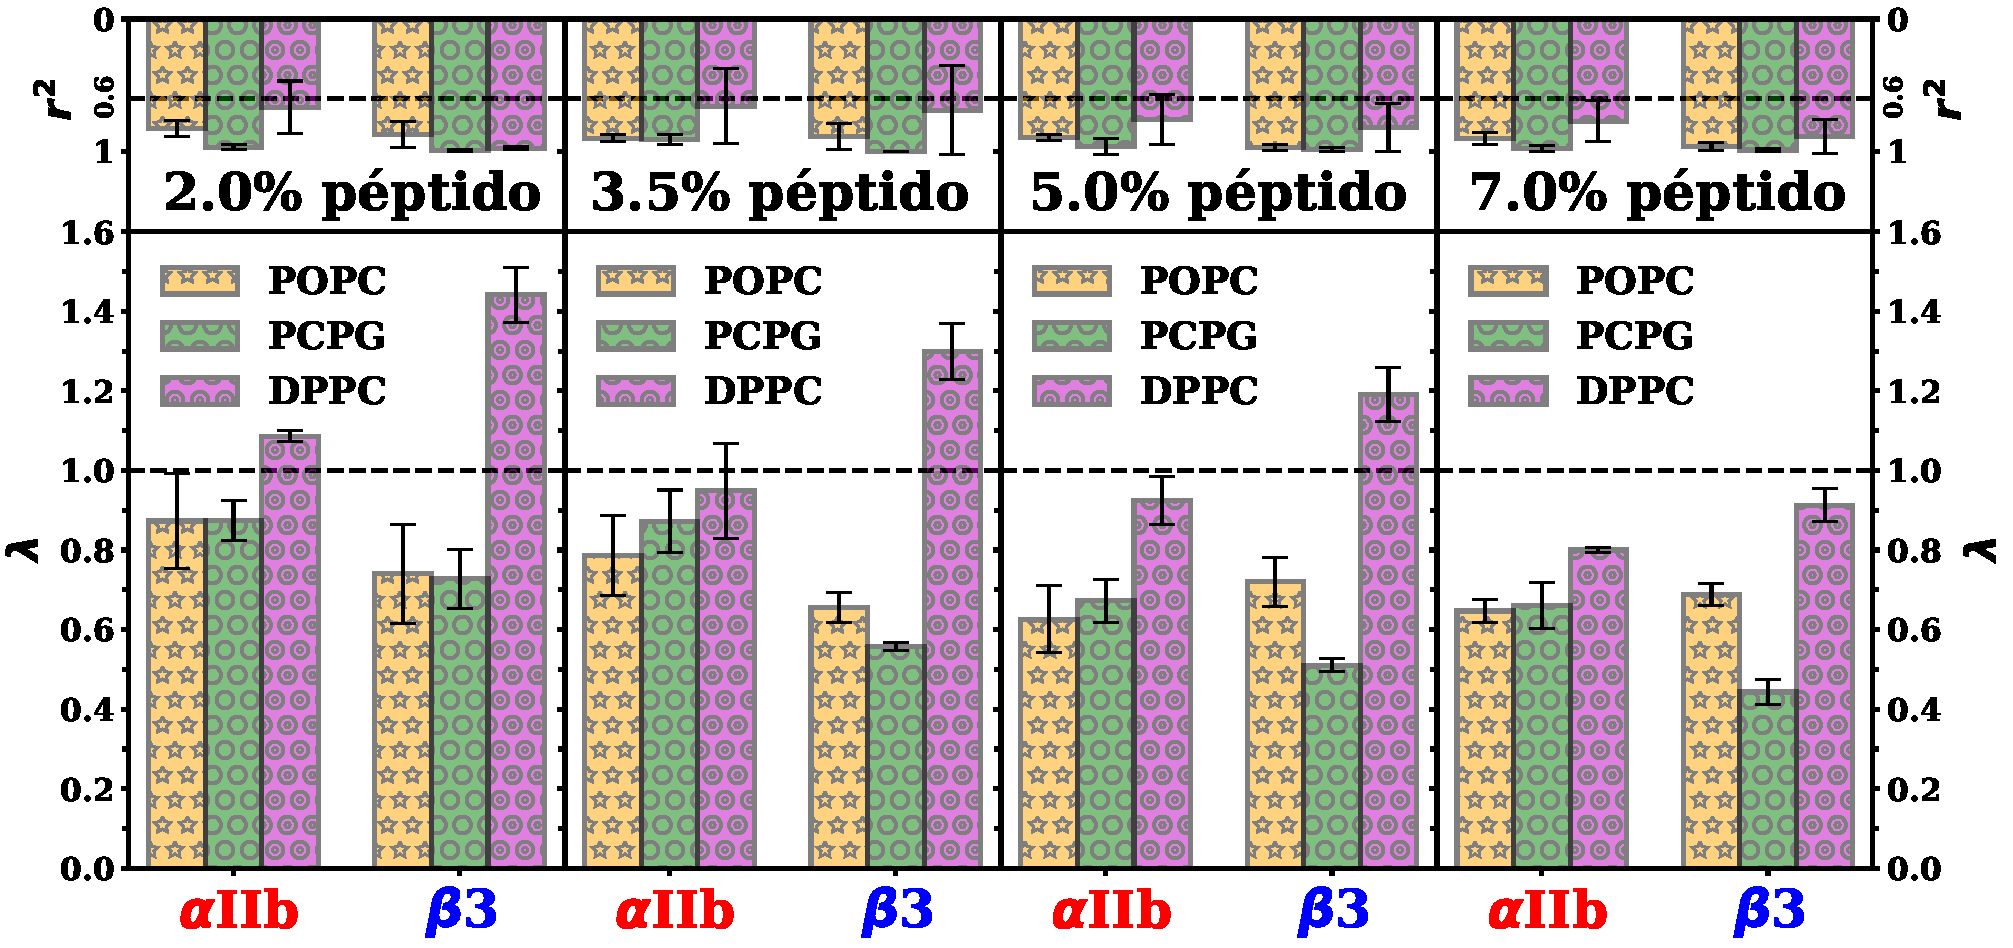
\includegraphics[width=0.99\linewidth]{fig/01_expe/mono/lambda_all2.pdf}
	\caption[Factor $\Lambda$ para las mezclas lípido-péptido.]{Factor $\Lambda$ para las mezclas lípido-péptido. Panel inferior valores de $\lambda$ para cada péptido en diferentes interfases lipídicas y panel superior los respectivos valores de r$^2$.}
        \index{lambda}
    \label{fig:lambda}
\end{figure}
%%%%%%%%%%%%%%%%%%%%% Fin %%%%%%%%%%%%%%%%%%%%%%%%


Se realizó este análisis con las isotermas de las mezclas lípido-péptido el cual se muestra en la \textbf{figura} \ref{fig:lambda}.  Observando los valores de r$^2$ (panel superior) en la mayoria de las mezclas   r$^2$ fue \textgreater{} 0.8, excepto para \ac{dppc} 
(\begin{tikzpicture}
            \node[draw, circle, fill=deepmagenta, line width=0.5pt, inner sep=3pt, scale=0.4, font=\color{black}] {\faCircle};
            \end{tikzpicture}) 
a 2.0\% y 3.5\% donde r$^2$ fue levemente \textgreater{} 0.6. Que r$^2$ se aproxime a 1 indica que las diferencias entre las isotermas reales e ideales están dadas principalmente por el valor de $\lambda$ y son independientes del rango de presión. Respecto al factor $\lambda$, el péptido $\beta$3  tiende a presentar valores de $\lambda$ \textgreater{} 1 en concentraciones de  2.0\% a 5.0\%, mientras que en presencia de $\alpha$IIb, $\lambda$ es ligeramente mayor a 1 cuando la concentración es 2.0\%. Antes se vió que a las dos presiones evaluadas los péptidos inducían una expansión (posiblemente interacciones repulsivas lípido-péptido) sobre la fase de éste lípido lo cual se reafirma con este análisis. Además con el valor agregado que se aprecia a nivel cuantitativo el efecto que induce cada péptido independiente de la presión superficial. Los valores menores de $\lambda$ se obtuvieron en las mezclas PCPG (\begin{tikzpicture}
  \node[draw, circle, fill=black, line width=0.2pt, inner sep=0.05pt, scale=0.6, font=\color{emerald}] {\faCircle}; 
  \end{tikzpicture})-$\beta$3, indicando la presencia de interacciones atractivas lípido-péptido y éstas se intensifican a medida que aumenta la concentración de péptido (disminuye $\lambda$; lo más probable es que el péptido $\beta$3 con carga positiva es atraído por la carga negativa del \ac{popg} en la mezcla PCPG. En cuanto a las mezcla \ac{popc}
  (\begin{tikzpicture}
  \node[draw, circle, fill=black, line width=0.2pt, inner sep=0.5pt, scale=0.4] {};
  \node[star, star point ratio=2.25, draw=black, fill=goldenpoppy, line width=0.2pt, minimum size=0.4cm, inner sep=0pt] {};
\end{tikzpicture})-péptido se obtuvieron valores intermedios respectos a las otras dos interfases, donde tanto $\alpha$IIb como $\beta$3  presentan interacciones atractivas con la interfase neutra.

Para enriquecer y profundizar el análisis de las isotermas de las mezclas lípido-péptido, es pertinente considerar los cambios conformacionales que los lípidos experimentan en respuesta a las distintas acomodaciones del péptido. Este fenómeno puede ser crucial para comprender las interacciones entre los componentes de la mezcla y cómo estas interacciones se modifican en función de la concentración del péptido y la naturaleza de la interfaz lípido-péptido.

Además, el concepto de compactación adquiere relevancia en este contexto. La compactación se refiere a la densificación de la monocapa lipídica inducida por la presencia y la interacción del péptido. Esta densificación puede resultar en un cambio en la movilidad y en la conformación de los lípidos, así como en la interacción entre los lípidos y los péptidos.


\section{Potencial de superficie y momento dipolar en mezclas lípido-péptido}\label{deltaV_mezclas}

Previamente en la \textbf{sección \ref{mono_pept_puros}}  se introdujo el concepto del potencial de superficie y momento dipolar. La \textbf{figura} \ref{fig:mu_dV_alfa} muestra el cambio del $\Delta$V en función del empaquetamiento molecular. Además, se estimó el momento dipolar perpendicular ($\mu_\perp$) empleando la ecuación \ref{ecu:potencial} el cual se muestra en el panel inferior de cada subfigura. Dado que $\Delta$V depende tanto de la densidad de empaquetamiento como de la orientación de las moléculas en la monocapa, se espera un aumento en los valores $\Delta$V durante la compresión de la fase LE como consecuencia de un progresivo  reordenamiento vertical. Este efecto se observó en las monocapas de \ac{dppc} ya que presenta diferentes fases a medida que se comprime, sin embargo, en presencia de péptido sea  \textbf{$\alpha$}IIb o  $\beta$3, disminuyen levemennte el $\Delta$V del lípido puro. La diferencia en valores de $\Delta$V entre las fases LE y LC ($\Delta$V$_{LC}$ -- $\Delta$V$_{LE}$) puede dar cuenta de repulsiones lípido-péptido como ya se mencionó anteriormente. Además se observó cómo la presencia de péptido cambia la forma del potencial del \ac{dppc} puro (señalados con las fechas \textcolor{black}{\faLongArrowRight}). En la interface neutra (\ac{popc}), el cambio del $\Delta$V por la presencia de péptido ($\alpha$IIb ó  $\beta$3) es ligeramente distinguible respecto al lípido puro; y con la interface cargada negativamente (mezcla binaria PCPG) se esperaba ver alguna diferencia notable entre el péptido $\alpha$IIb y $\beta$3 dado que estos tiene carga neta diferente, pero lo observado fue un cambio muy pequeño en presencia de $\beta$3. Esta observación podría atribuirse a la complejidad inherente al control experimental de los rearreglos estructurales y moleculares, así como a la incertidumbre intrínseca en las mediciones realizadas \cite{Brockman1994}. 
El $\mu_\perp$ para \ac{popc} y \ac{dppc} se muestra en la \textbf{figura} \ref{fig:mu_dV_alfa}A-B (panel inferior) en ausencia y presencia de ambos péptidos, cuando el área molecular $\Xapprox 225$  Å\textsuperscript{2}, el $\mu_\perp$ inicia con  valores más altos respecto al $\mu_\perp$  los lípidos puros, y esto se debe a lo ya mencionado, donde a área grandes los péptidos tienen suficiente libertad para tender a orientarse paralelamente a la superficie y por lo tanto, habrán más aminoácidos que entran en contacto con el agua los cuales contribuyen al incremento del $\mu_\perp$. A medida que se comprime lateralmente, los péptidos se reorientan verticalmente, por lo tanto, se observa un decrecimiento paulatino del  $\mu_\perp$ hasta llegar a valores similares que alcanza el lípido puro cuando han colapsado. Con la interfase de PCPG sucedio lo contrario, especialmente en presencia de $\beta$3, donde a áreas mayores el $\mu_\perp$ del lípdio es mayor respecto a las mezcla con $\beta$3. En general para las mezclas lípido-péptido llama la atención en todos casos, siempre se llegó valores similares de la interface puro, al similar fue reportado por Le--Thu Nguyen et al. \cite{Nguyen2010}, donde se observó que el $\mu_\perp$ de diferentes polipéptidos $\alpha$ hélice es significativamente suprimido en soluciones acuosas debido al efecto de la esfera de solvatación de moléculas de agua que pueden formar puentes de hidrógeno con los grupos carbonilos de los péptidos específicamente cuando se encuentran ``paralelo'' a la superficie, luego al comprimirse los $\mu_{H_{2}O}$ se orientan hacia abajo, dando como resultado la diminución del $\mu_\perp$. Además, si consideramos que ambos péptidos tienen resíduos del domino \ac{ic} en la subfase, el $\mu_{péptido}$ de esos residuos ya se encuntran ``apantallados'', por lo tanto, no contribuyen al $\mu_\perp$.


%%%%%%%%%% Potencial y dipolo mezclas %%%%%%%%%%%%

\begin{figure}[H] % supposedly places it here ...
    \centering
	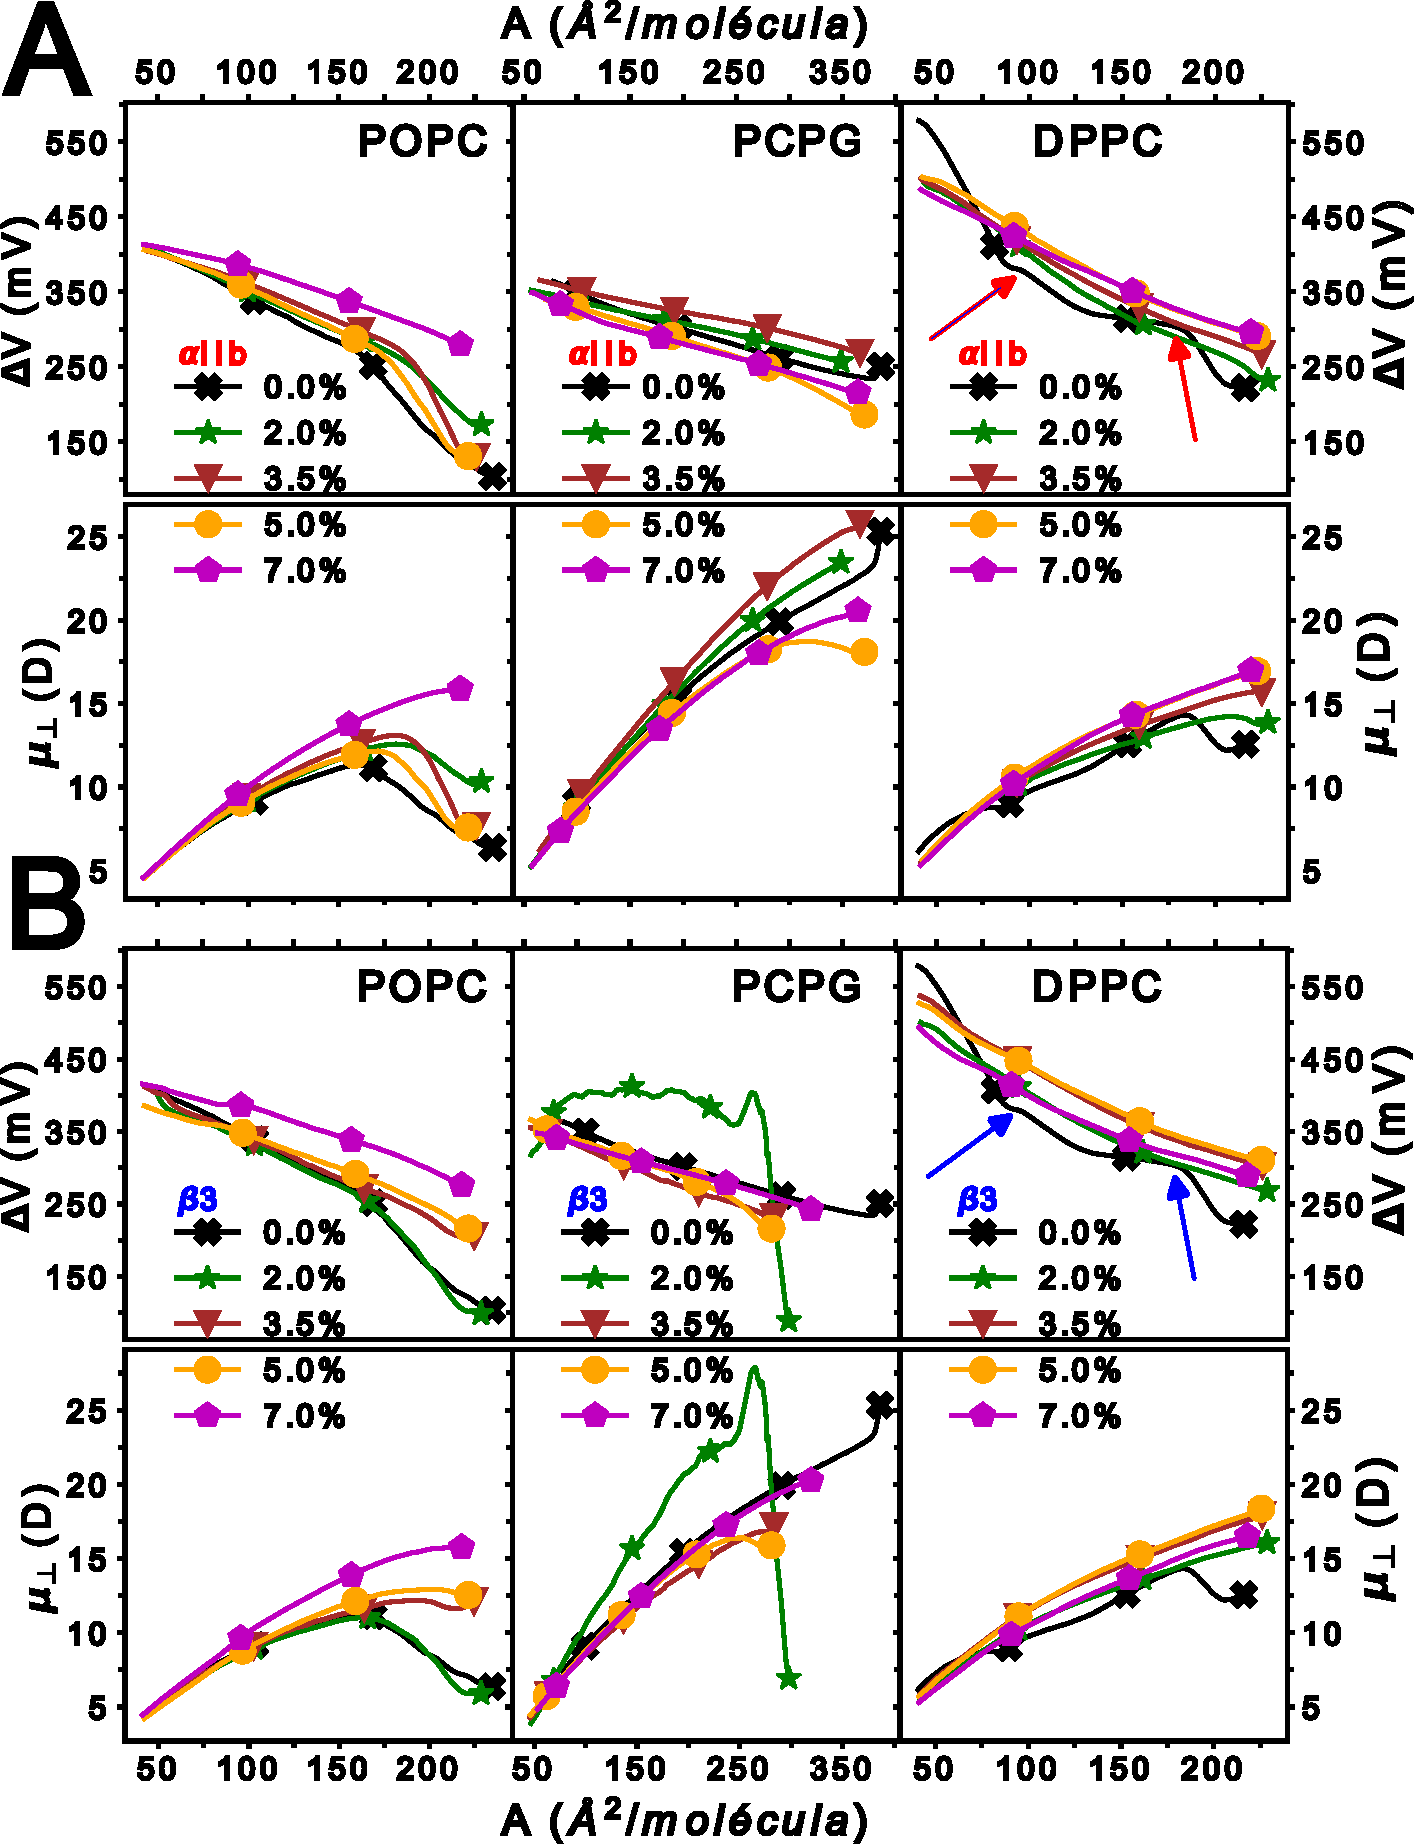
\includegraphics[width=0.99\linewidth]{fig/01_expe/mono/mu_dipolo_deltaV_all.pdf}
	\caption[Potencial de superficie y momento dipolar para las mezclas lípido-péptido]{Potencial de superficie ($\Delta$V)  y momento dipolar perpendicular ($\mu_\perp$) para las mezclas lípido-péptido en función del área molecular promedio (\textbf{A}). A) $\Delta$V (panel superior) y $\mu_\perp$ (panel inferior) para las mezclas lípido/$\alpha$IIb. B) $\Delta$V (panel superior) y $\mu_\perp$ (panel inferior) para las mezclas lípido/$\beta$3.}
        \index{mu_dV_alfa}
    \label{fig:mu_dV_alfa}
\end{figure}
%%%%%%%%%%%%%%%%%%%%% Fin %%%%%%%%%%%%%%%%%%%%%%%%



\section{Análisis de la elasticidad lateral}
%%https://www.cell.com/biophysj/pdf/S0006-3495(97)78226-2.pdf
%%%Leer bien para posible análisis extra del módulo
%%%https://hal.science/hal-04037820/document

La membrana celular es una organización compleja y muy dinámica. Su integridad y funcionalidad dependen de la flexibilidad estructural de sus componentes. La mutua influencia entre componentes, principalmente lípidos y proteínas, puede modular la deformación, los cambios en radios y curvatura, cambios en el espesor de la membrana. Particularmente, la compresibilidad lateral de la membrana es un parámetro que describe sus propiedades mecánicas y puede ser controlada por la composición de la membrana y/o por la presencia de proteínas que inducen estos cambios \cite{Evans1976}. Para examinar la rigidez lateral de las monocapas, específicamente en las mezclas lípido-péptido, se calculó el módulo de compresibilidad (C$_s^{\text{--}1}$) usando los datos de las curvas $\pi \text{--}$\textit{A} (\textbf{figura} \ref{fig:area_pi_all})  basado en la ecuación \ref{ecu:Cs}, 

\begin{equation}\label{ecu:Cs}
    C_s^{\text{--}1} =  \text{--} A \left(\frac{d\pi}{dA} \right)  
\end{equation}

Donde \textit{A} es el área por molécula a la presión superficial  $\pi$. El C$_s^{\text{--}1}$ provee información acerca de la conformación estructurada de los lípidos y la rigidez de la monocapal. Lípidos con una conformación estructurada (fase LC), presentarán valores de C$_s^{\text{--}1}$ altos, mientras que si presentan un cierto grado de heterogeneidad estructural (fase LE), C$_s^{\text{--}1}$ tendrá valores bajos. Valores cercanos a cero de C$_s^{\text{--}1}$, corresponden una interfase de agua pura, libre de monocapas. Si hay un incremento en su magnitud estará dada por la actividad superfical de las moléculas presentes en la interface, cuando el valor C$_s^{\text{--}1}$ es grande, significa que la monocapa es menos compresible. Valores de C$_s^{\text{--}1}$ cercanos a cero corresponden a una interfase de agua pura, libre de monocapa. La fase \ac{le} se caracteriza por presentar una C$_s^{\text{--}1}$ entre 12-50 mN/m, y valores entre 100-250 mN/m corresponde a una fase LC \cite{Hadjittofis2017}. La \textbf{figura} ~\ref{fig:CsPi} muestra los curvas de compresibilidad tanto para los componentes puros como las mezlcas lípido-péptido, lípido-$\alpha$IIb se observan al lado derecho y al lado izquierdo lípido-$\beta$3.
%%2019_Agata_Ladniak.pdf 
Respecto a los péptidos puros, ambos alcanzan rápidamente C$_s^{\text{--}1}$ $\Xapprox$  30 mN/m y permanece oscilando en ese valor hasta presiones altas. Además, los dos péptidos presentan un pequeño decrecimiento de C$_s^{\text{--}1}$ alrededor de los 28 mN/m y 32 mN/m para $\alpha$IIb y $\beta$3, respectivamente. Este mínimo podría atribuirse a una reorganización estructural de los péptidos en la interfase tal como se mencionó en las \textbf{secciones \ref{sect:mono_mezclas}} y \textbf{\ref{deltaV_mezclas}} \hl{(buscar refencias de Cs para péptidos mostrar con flecha en la gráfica el minimo de los péptidos y del dppc)}.
Observando los C$_s^{\text{--}1}$ para \ac{popc} puro, éste alcanza valores máximos hasta $\Xapprox$ 50 mN/m (valores característicos para una fase LE) y una vez alcanza la presión de colapso decae. En general en presencia de péptido $\alpha$IIb  o $\beta$3 el C$_s^{\text{--}1}$ disminuye respecto al lípido puro y éste efecto es más marcado con $\beta$3. 
Con la interfase que tiene un 30\% mol de \ac{popg}, éste disminuyó C$_s^{\text{--}1}$ del \ac{popc} puro, donde esta mezcla PCPG presentó un C$_s^{\text{--}1}$ de  $\Xapprox$ 30 mN/m, valor muy similar al de los péptidos (\textbf{figura} ~\ref{fig:CsPi} panel del medio). En prencia de péptido, éstos tienden a disminuir la compresibilidad del PCPG puro sutilmente, siendo $\alpha$IIb  el péptido que induce un mayor efecto.
Finalmente en la interfase con \ac{dppc}, para el lípido puro se observan dos estados, el primero alcanza un valor de C$_s^{\text{--}1}$  $\Xapprox$ 25 mN/m, éste primer estado corresponde a la coexistencia de fase LE--LC \hl{buscar REF}. Posteriormente se produce un aumento pronunciado del C$_s^{\text{--}1}$ con el amento de la $\pi$ hasta alcanzar valores de C$_s^{\text{--}1}$  mayores a 100 mN/m, el cual se atribuye un estado de fase LC. Cuando se adiciona péptido ya sea $\alpha$IIb o $\beta$3, ambos disminuyen la compresibilidad del lípido drasticamente, incluso a bajas comcentraciones del 2.0\% de péptido pasa a tomar valores cercanos a $\Xapprox$ 50 mN/m, donde $\beta$3 es el más disminuye C$_s^{\text{--}1}$.

Para finalizar en la \textbf{tabla} \ref{tab:resum_mono} se muestras un resumen de las propiedades de todas las monocapas estudiades en éste trabajo, se tomó como referencia una presión de 30 mN/m.

%%%%%%%%%%%%%%%%%%%Tabla resumen%%%%%%%%%%%%%%%%%%%%%%%%
% Please add the following required packages to your document preamble:
% \usepackage{booktabs}
% \usepackage{multirow}
\begin{table}[H]
\centering
%\begin{adjustbox}{width=1\textwidth}
\caption{Resumen propiedades  monocapas a una presión de 30 mN/m.\hl{Falta completar} }\label{tab:resum_mono}
\resizebox{\textwidth}{!}{
\begin{tabular}{@{}cclllllllllll@{}}

\toprule
\multirow{2}{*}{Péptido} & \multirow{2}{*}{\%}  & \multicolumn{3}{c}{$\mu_\perp$ (D)}  & \multicolumn{1}{p{0.01mm}}{}  & \multicolumn{3}{c}{C$_s^{\text{--}1}$ (mN/m)} & \multicolumn{1}{p{0.01mm}}{}  & \multicolumn{3}{c}{A (Å\textsuperscript{2})} \\ 

\cmidrule(lr){3-5} \cmidrule(lr){7-9} \cmidrule(l){11-13}  
                         &                      & \multicolumn{1}{c}{POPC} & \multicolumn{1}{c}{PCPG} & \multicolumn{1}{c}{DPPC} & \multicolumn{1}{p{0.01mm}}{} & \multicolumn{1}{c}{POPC} & \multicolumn{1}{c}{PCPG} & \multicolumn{1}{c}{DPPC} & \multicolumn{1}{p{0.01mm}}{} & \multicolumn{1}{c}{POPC} & \multicolumn{1}{c}{PCPG} & \multicolumn{1}{c}{DPPC} \\ 
                         
                                                
\cmidrule(lr){1-2} \cmidrule(lr){3-5} \cmidrule(lr){7-9} \cmidrule(l){11-13}

- - -     		& 0.0					& ab\textpm 0.01		& ab\textpm 0.00		& ab\textpm 0.00		& 	&54.96\textpm b		& 36.39\textpm b		& 130.80\textpm b& &	73.69\textpm 3.70 & 100.51\textpm 4.35 &  39.06\textpm 0.55 
\vspace{3mm} \\

$\alpha$IIb     & \multirow{2}{*}{2.0}   &  6.64\textpm 0.01 	& 9.86\textpm 0.00	& 9.71\textpm 0.00	& 	& 44.92\textpm b		& 30.13\textpm b		& 63.23\textpm b	& & 65.30\textpm 2.31 	& 75.32\textpm 2.63& 58.36\textpm 0.06\\ 
$\beta$3        & 						&  7.50\textpm 0.00 	& 12.03\textpm 0.12	& 10.03\textpm 0.01	& 	& 47.12\textpm b		& 34.28\textpm b		& 46.28\textpm b	& &	61.98\textpm 2.42 	& 72.45\textpm 5.64& 63.80\textpm 0.07                          
\vspace{3mm}\\

$\alpha$IIb     & \multirow{2}{*}{3.5} 	&  8.70\textpm 0.00	& 10.56\textpm 0.07	& 10.21\textpm 0.00	& 	& 45.45\textpm b		& 27.30\textpm b		& 52.51\textpm b	& &	74.24\textpm 0.55	& 90.15\textpm 24.02& 60.94\textpm 0.81\\
$\beta$3        & 						&  7.40\textpm 0.00	& 8.19\textpm 0.07	& 11.88\textpm 0.00	& 	&53.41\textpm b		& 38.27\textpm b		& 41.73\textpm b	& &	65.02\textpm 1.43 	&65.04\textpm 0.67& 69.83\textpm 7.57                           
\vspace{3mm} \\

$\alpha$IIb     & \multirow{2}{*}{5.0}   &  8.68\textpm 0.00	& 8.71\textpm 0.03	& 11.36\textpm 0.00	& 	&49.57\textpm b		& 31.39\textpm b		& 51.91\textpm b	& &	71.41\textpm 6.89 	&77.62\textpm 5.07& 65.76\textpm 1.74\\
$\beta$3        & 						&  7.61\textpm 0.00	& 7.31\textpm 0.00	& 12.77\textpm 0.01	& 	&33.06\textpm b		& 32.27\textpm b		& 44.45\textpm b	& &	74.34\textpm 3.09 	& 59.47\textpm 1.06& 71.83\textpm 1.51                          
\vspace{3mm} \\

$\alpha$IIb    & \multirow{2}{*}{7.0}  	&  9.89\textpm 0.00	& 10.53\textpm 0.00	& 11.51\textpm 0.00	& 	&45.63\textpm b		& 32.72\textpm b		& 47.61\textpm b	& &	81.54\textpm 0.89 	&85.71\textpm 4.51& 64.21\textpm 0.41\\
$\beta$3       & 						&  9.06\textpm 0.00	& 9.33\textpm 0.31	& 10.24\textpm 0.00	& 	&31.09\textpm b		& 31.85\textpm b		& 43.02\textpm b	& &	76.34\textpm 1.32 	& 59.57\textpm 13.07& 68.88\textpm 1.94  \\ 
\bottomrule
\end{tabular}
}
\end{table}                        
%%%Fin Tabla resumen%%%


%%%%%%%%%% Figura Módulo de compresibilidad %%%%%%%%%%%%

\begin{figure}[H] % supposedly places it here ...
    \centering
	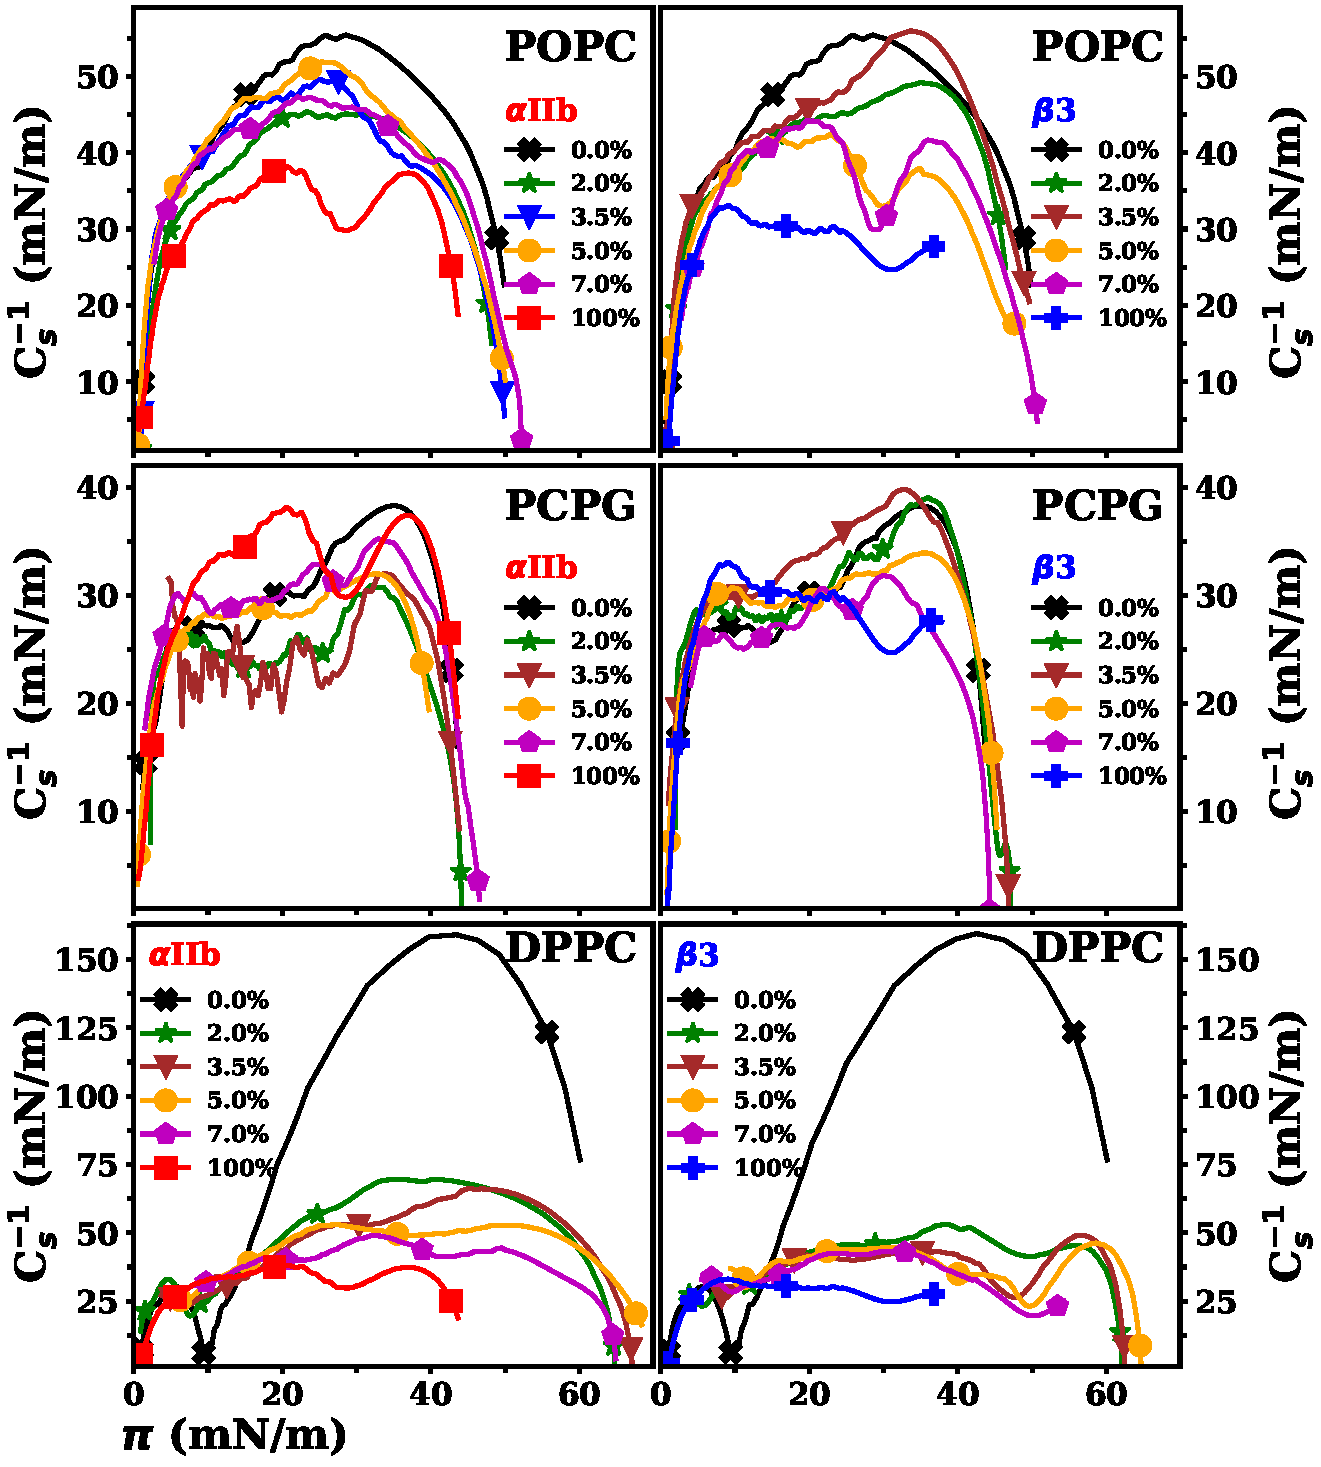
\includegraphics[width=0.99\linewidth]{fig/01_expe/mono/cs_all.pdf}
	\caption[Módulo de compresibilidad  en fucnión de la presión superficial en la interfase aire-agua.]{Módulo de compresibilidad (C$_s^{\text{--}1}$ ) en función de la presión superficial ($\pi$) en la interfase aire-agua. Al lado izquierdo lípido/$\alpha$IIb y lado derecho lípido/$\beta$3.}
        \index{CsPi}
    \label{fig:CsPi}
\end{figure}
%%%%%%%%%%%%%%%%%%%%% Fin %%%%%%%%%%%%%%%%%%%%%%%%


%%%%%%%%% Ciclos compresion-Expansión%%%%%%
\section{Discusión general del capítulo}

Para resumir de forma gráfica los resultados observados anteriormente, la \textbf{figura} \ref{fig:esquema_final} ilustra lo planteado en cada sistema. Se mencionó que la orientación de los péptidos puros en monocapas de Langmuir es perpendicular al plano de las monocapas, preferentemente. Donde al inicio a presiones bajas éstos presentan una conformación acostada sobre la fase acuosa pero a medida que se comprime lateralmente, éstos se orientan verticalemente. Además, dicha orientación es en dirección del N al C terminal debido a que los dos péptidos tienen resíduos polar en la región del C terminal que pueden interactuar favorablemente con el agua, mientras que la región del N terminal tiene un carácter más hidróbico que podría presentar interacciones poco favorables con el agua. También se mencionó que esta región del C terminal que está en contacto con la interfase, posiblemente presenta rearreglos de estructura secundaria de tal forma que a medida que se comprime, esta región adopta una estructura helicoidal donde algunos residuos polares contribuyen al potenecial de superficie. Respecto al efecto que inducen los péptidos $\alpha$IIb/$\beta$3 sobre monocapas de lípidos, en la caso de la interfase neutra y de características de \ac{le}, ambos péptidos inducen un efecto de compactación, es decir, hay presecia de interacciones lípido-péptido atractivas que llevan la monocapa a un estado más compacto respecto a la monocapa del lípido puro. Si a la misma interfase se le agrega un 30\% de lípido con carga negativa como es el \ac{popg}, los péptidos inducen un efecto opuesto, mencionado anteriormente, es decir, se observó una interacción repulsiva, siendo esta mayor en presencia de $\beta$3. Por otra parte, cuando los péptidos estan en una interfase lípidica neutra pero con cadenas saturadas como el \ac{dppc}, estos inducen un efecto repulsivo sobre la monocapa de los lípidos, incluso para ésta interfase se vio que ya con un 2\% de péptido disminuye drásticamente la compresiblidad respecto al lípido puro, miestras que las compresibilidades de las interfaces \ac{popc} y PCPG también dismuyen pero el efecto es menos marcado que con \ac{dppc}.

\begin{figure}[h] % supposedly places it here ...
    \centering
	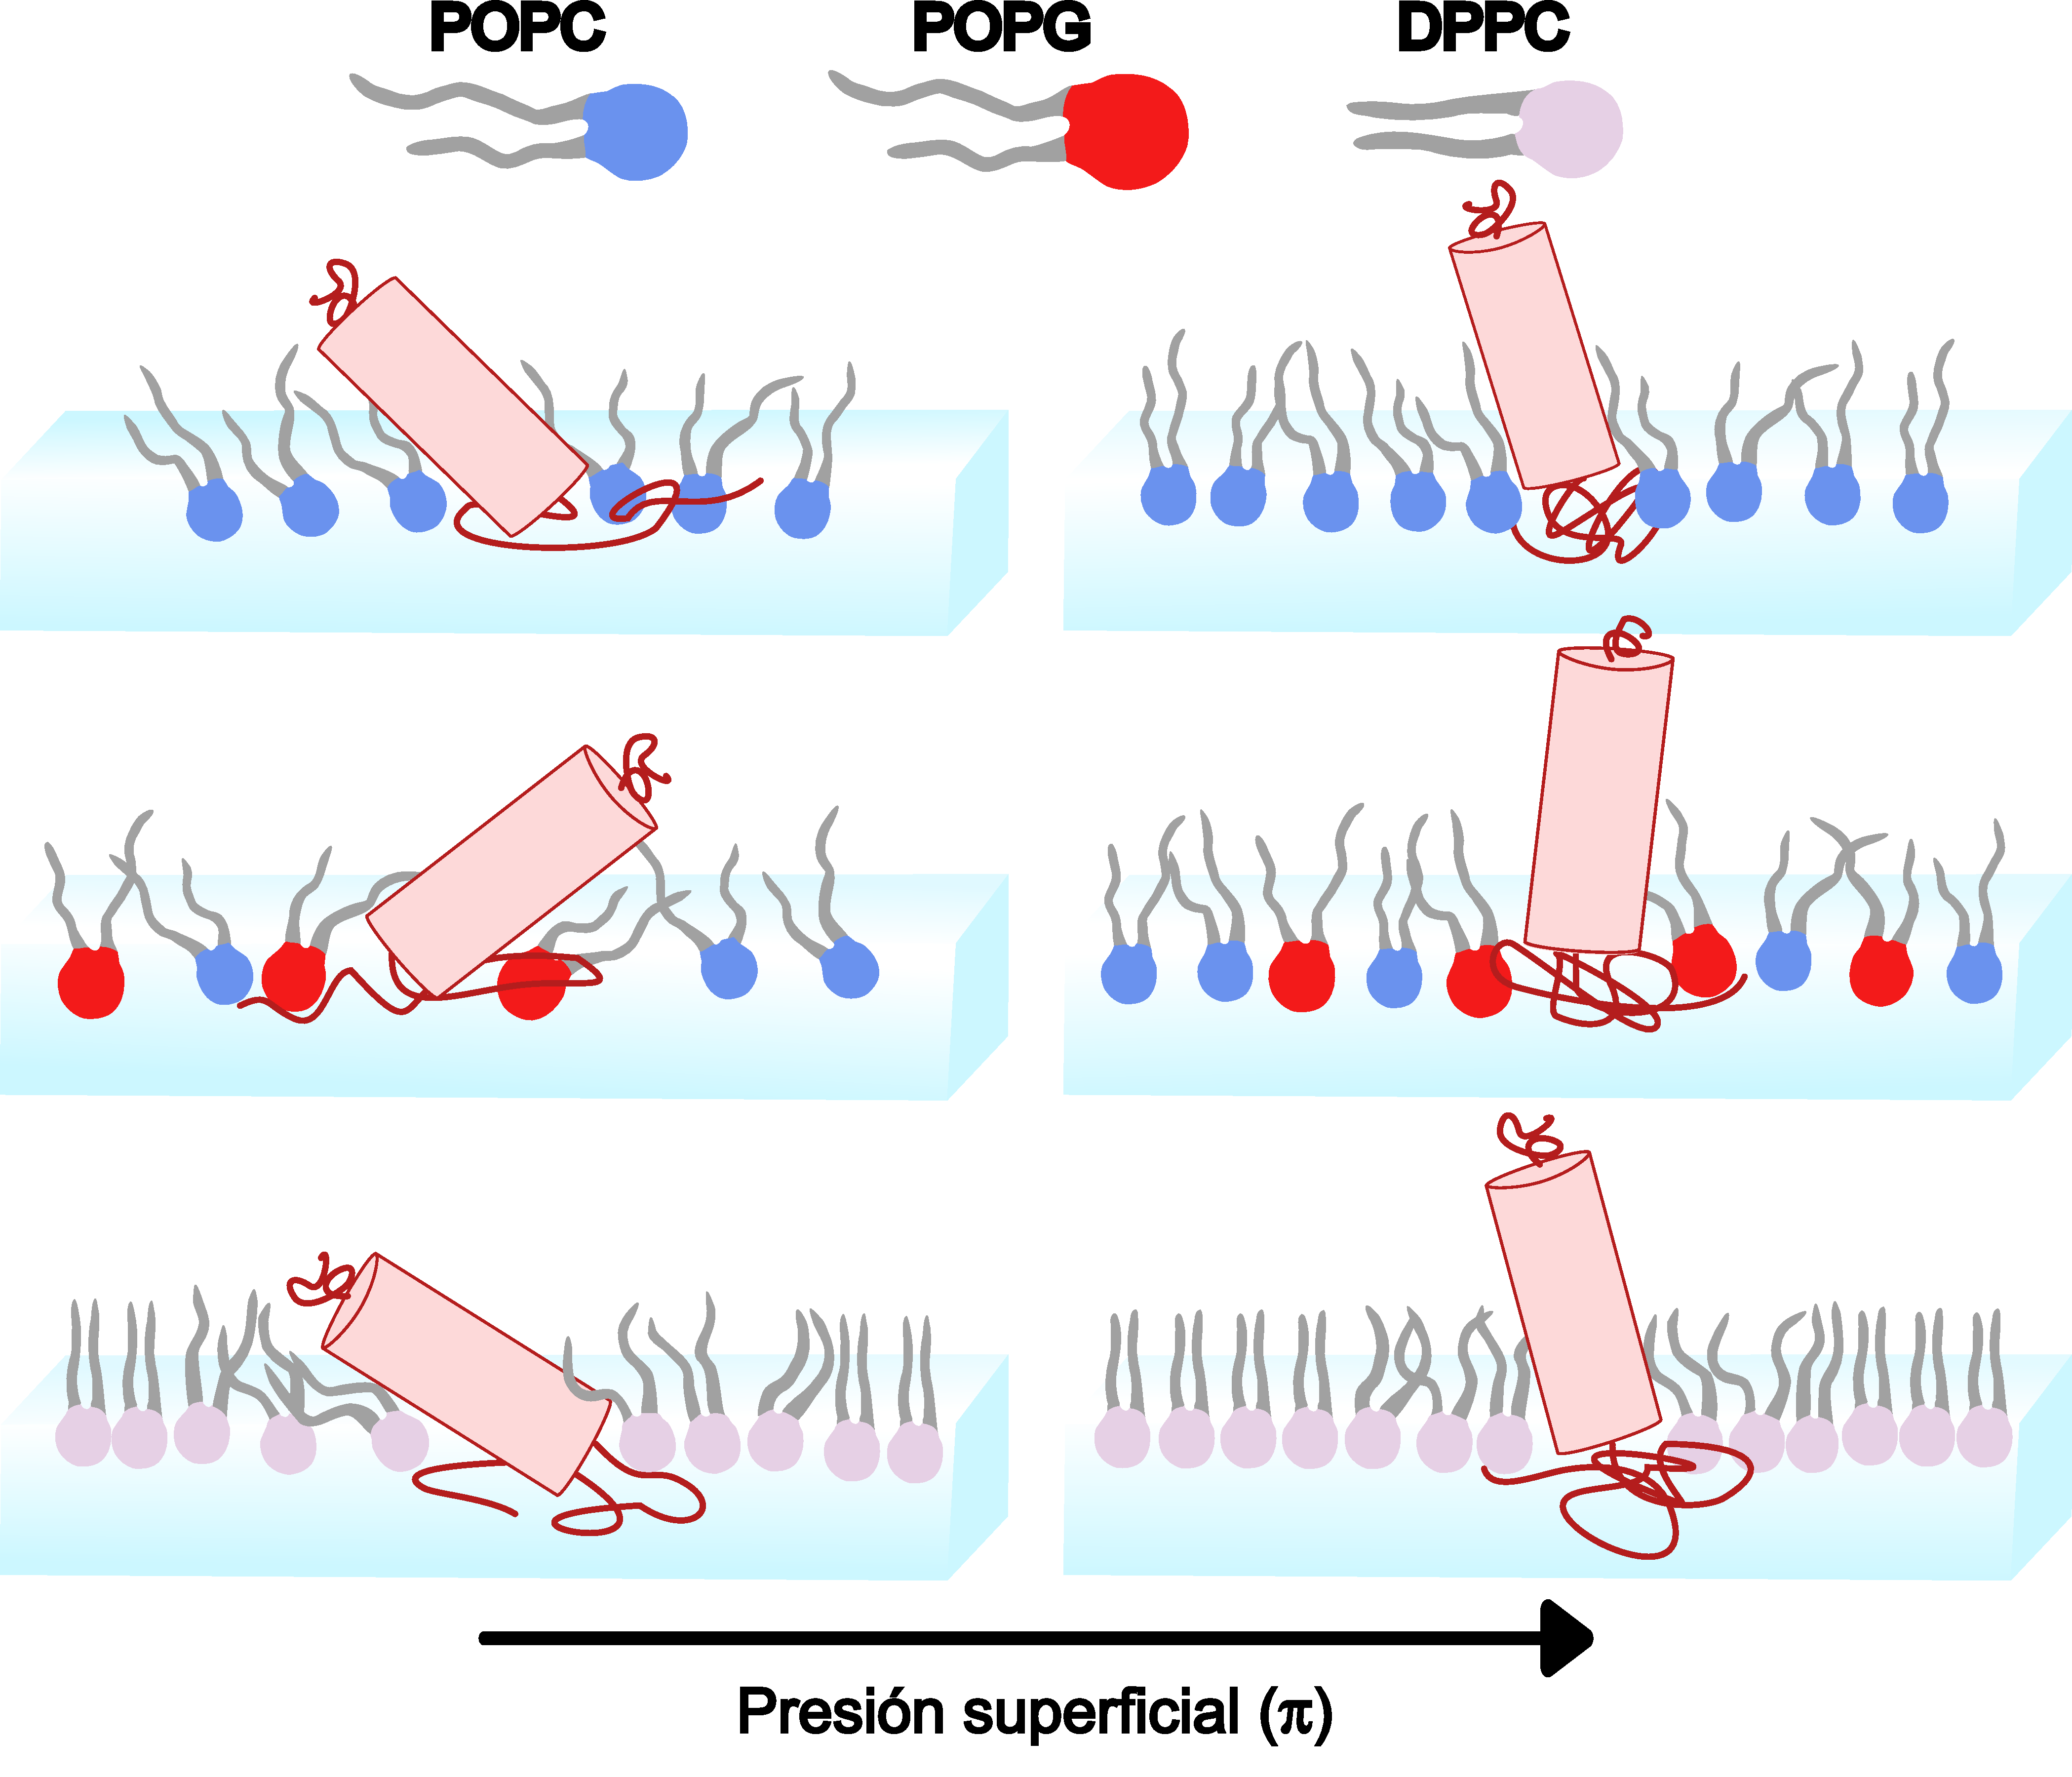
\includegraphics[width=0.99\linewidth]{fig/01_expe/esquema_final_lipido-peptido.pdf}
	\caption[Esquema de interacción lípido-péptido en monopas]{Esquema de interacción lípido-péptido en monopas. A la izquierda representación en condiciones iniciales de presión superficial cercano a cero; a la derecha, reorganización molecular a presiones altas.}
        \index{test}
    \label{fig:esquema_final}
\end{figure}
%%%%%%%%%%%%%%%%%%%%%% Fin %%%%%%%%%%%%%%%%%%%%%%%%
%
\chapter{Conformación de segmentos \ac{tm}-\ac{ic} de integrinas $\alpha$IIb/$\beta$3: Rol del ambiente lipídico}\label{chap:dm}

El ambiente lipídico en el cual se encuentran las proteínas de membrana, puede cambiar sus propiedades biofísicas por diferentes vías, sin embargo se resaltan dos principalmente, variación de las propiedades fisicoquímicas de la bicapa, y através de interacciones moleculares entre las moléculas que la componen \hl{REF}. La presencia de proteínas puede inducir la formación de un ``anillo'' de lípidos al rededor de la proteína.  Los lípidos que se encuentran en este anillo disponen de menor libertad de movimiento  comparado a los lípidos que se encuentran más alejados, también su orientación respecto a la normal de la bicapa se podría ver afecto según cuánto interaccione con la proteína \hl{REF}. En cuanto a las proteínas de membrana al estar confinadas en un ambiemte altamente hidrofóbico, pueden adoptar dos tipos de estructura, hélice $\alpha$ o barril $\beta$. Las hélice $\alpha$ 





%%%%%%%%%%% Figura %%%%%%%%%%%%
\begin{figure}[H]
    \centering
	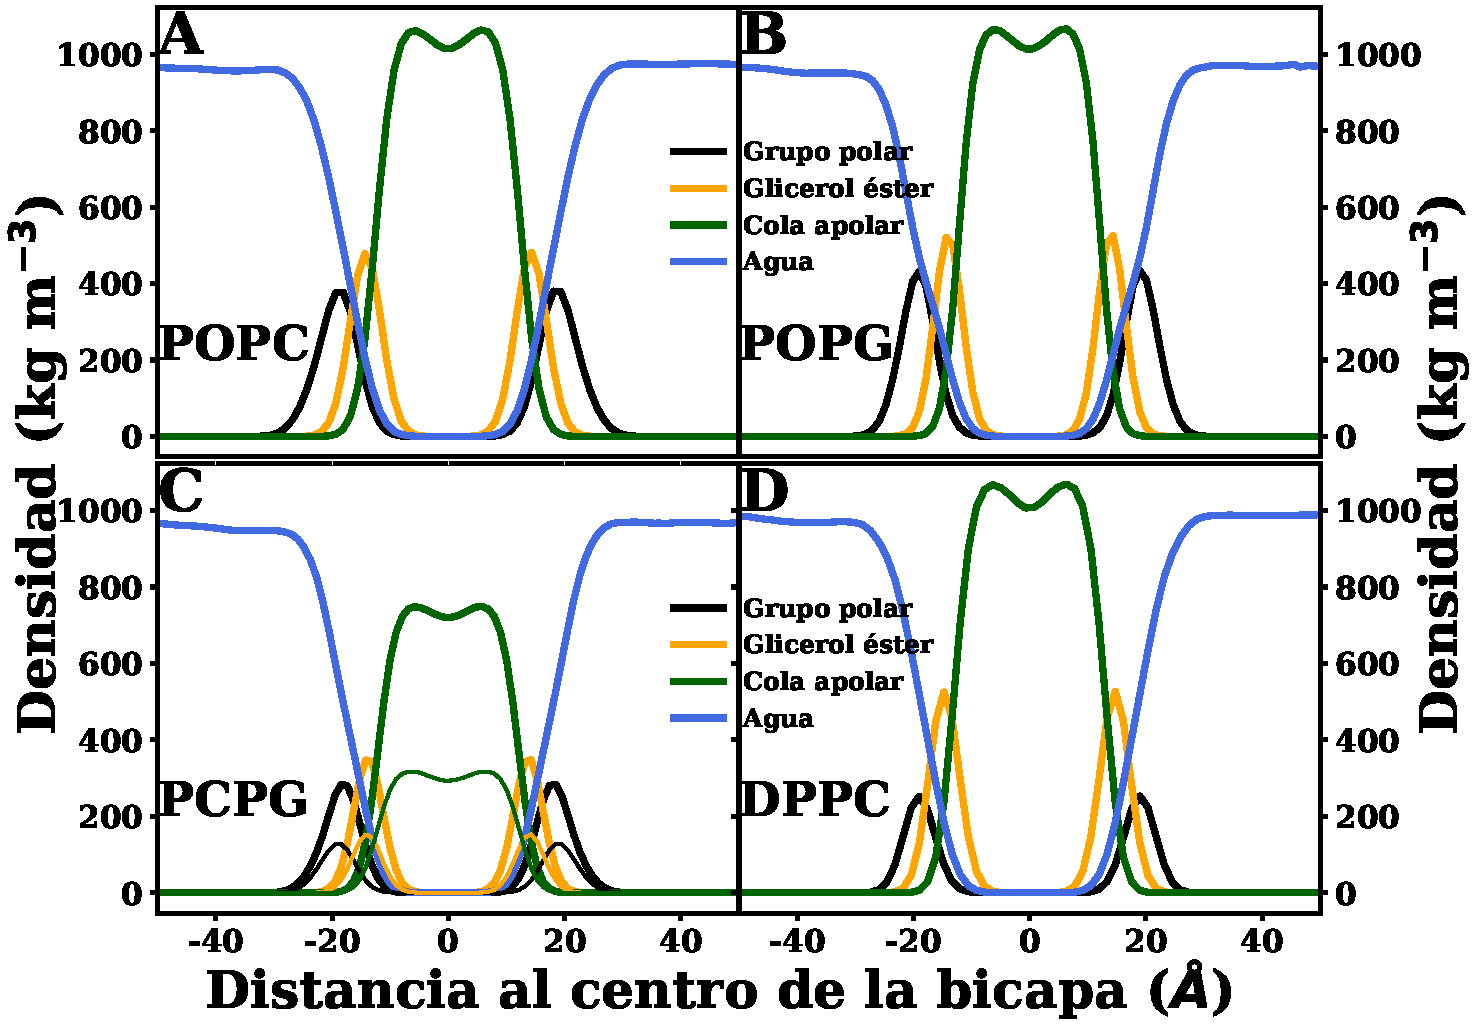
\includegraphics[width=1\linewidth, height=0.8\textheight, keepaspectratio]{fig/02_dm/density_all.pdf} 
	\caption[]{Distrubuciónd e densidad de grupos  \textbf{a-b-c-d)} POPC, DPPC y PCPG}
      \index{density}
    \label{fig:densidad}
\end{figure}
%%%%%%%%%%%%%%%%%%%%%%% Fin %%%%%%%%%%%%%%%%%%%%%%%%


%%%%%%%%%%% Figura %%%%%%%%%%%%
\begin{figure}[H]
    \centering
    \begin{subfigure}[t]{0.45\textwidth}
        \centering
        \subcaption{}
        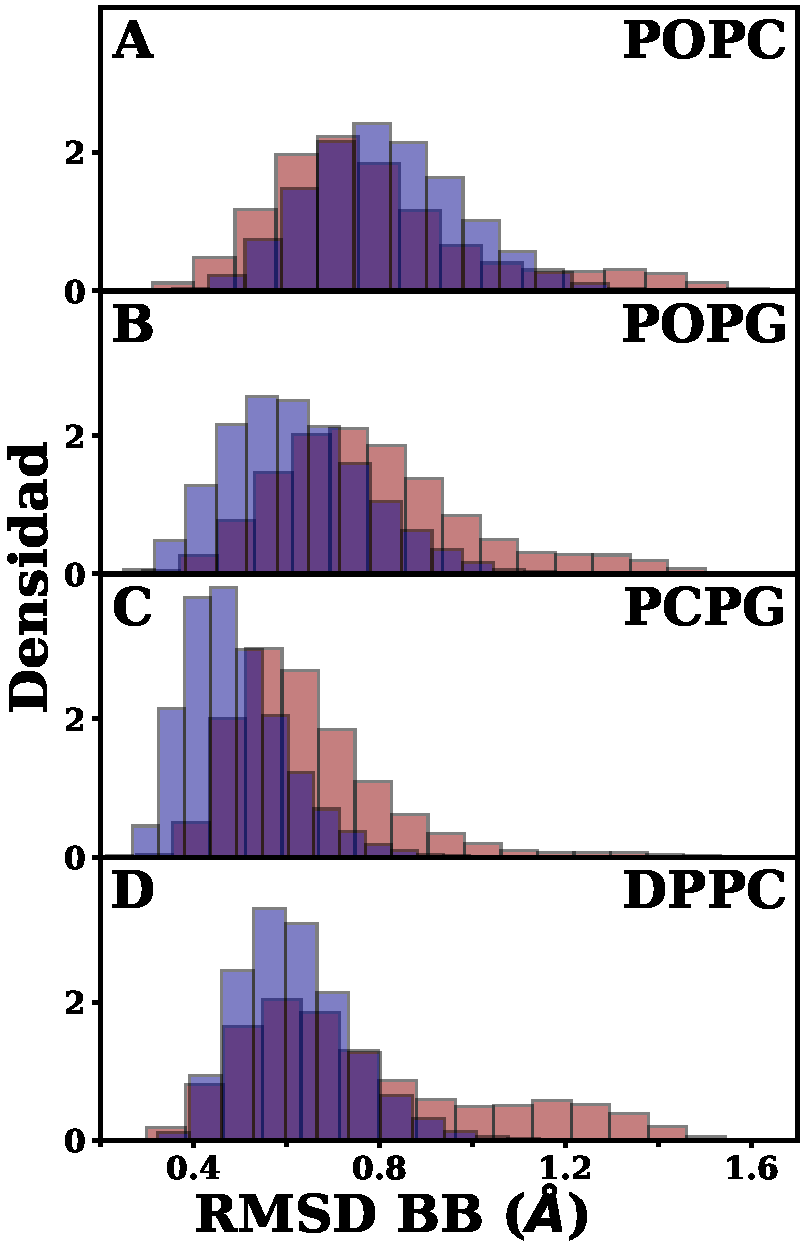
\includegraphics[width=1\linewidth, height=0.99\textheight, keepaspectratio]{fig/02_dm/rmsd_all.pdf} 
    \end{subfigure}
    \begin{subfigure}[t]{0.45\textwidth}
        \centering
        \subcaption{}
        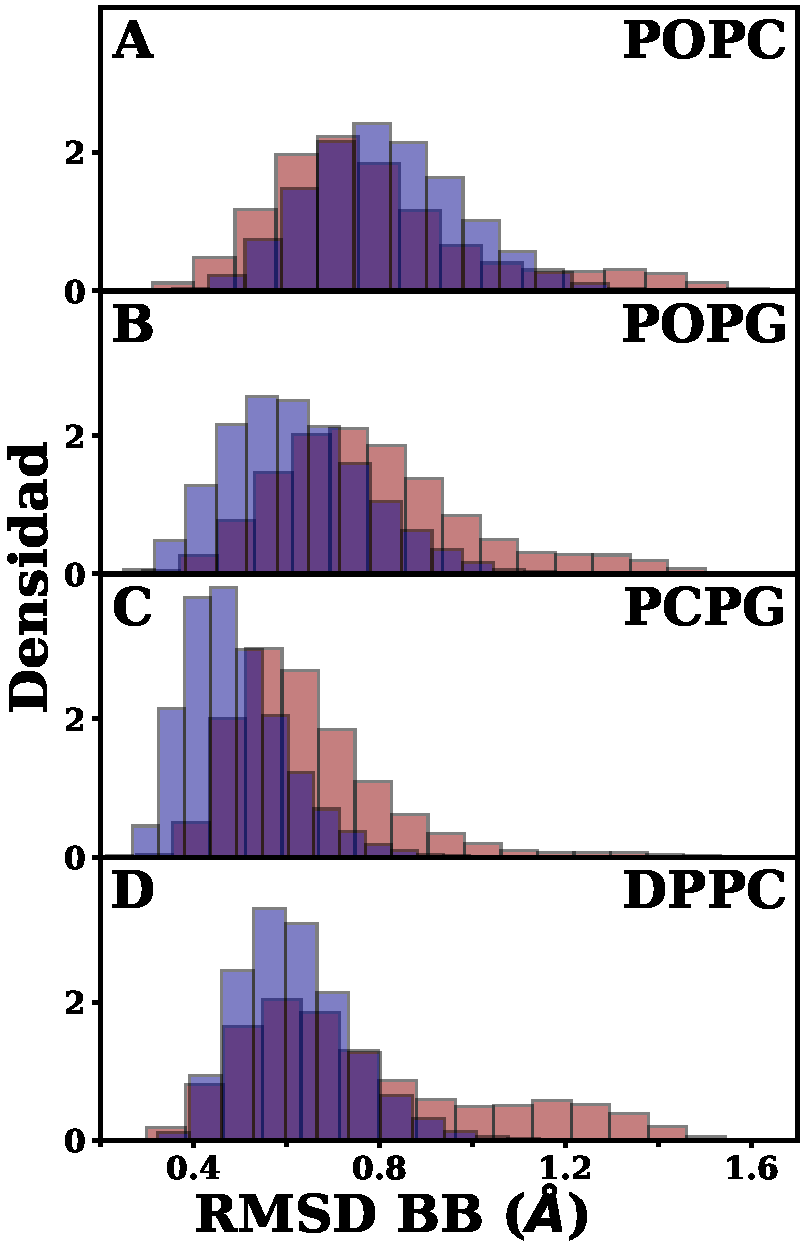
\includegraphics[width=1\linewidth, height=0.99\textheight, keepaspectratio]{fig/02_dm/rmsd_all.pdf}     
    \end{subfigure}
    
\caption[Histograma del RMSD  y \hl{FMSF} de los C$_\alpha$ del dominio transmenbrana $\alpha$IIb/$\beta$3]{Histograma del RMSD  y \hl{FMSF} de los C$_\alpha$ del dominio transmenbrana del dímero $\alpha$IIb/$\beta$3. En cada panel el color rojo y azul representan el péptido $\alpha$IIb y $\beta$3, respectivamente.}
        \index{rmsdf}
    \label{fig:rmsdf}
\end{figure}
%%%%%%%%%%%%%%%%%%%%%%% Fin %%%%%%%%%%%%%%%%%%%%%%%%


%%%%%%%%%%% Figura %%%%%%%%%%%%
\begin{figure}[H]
 \centering
	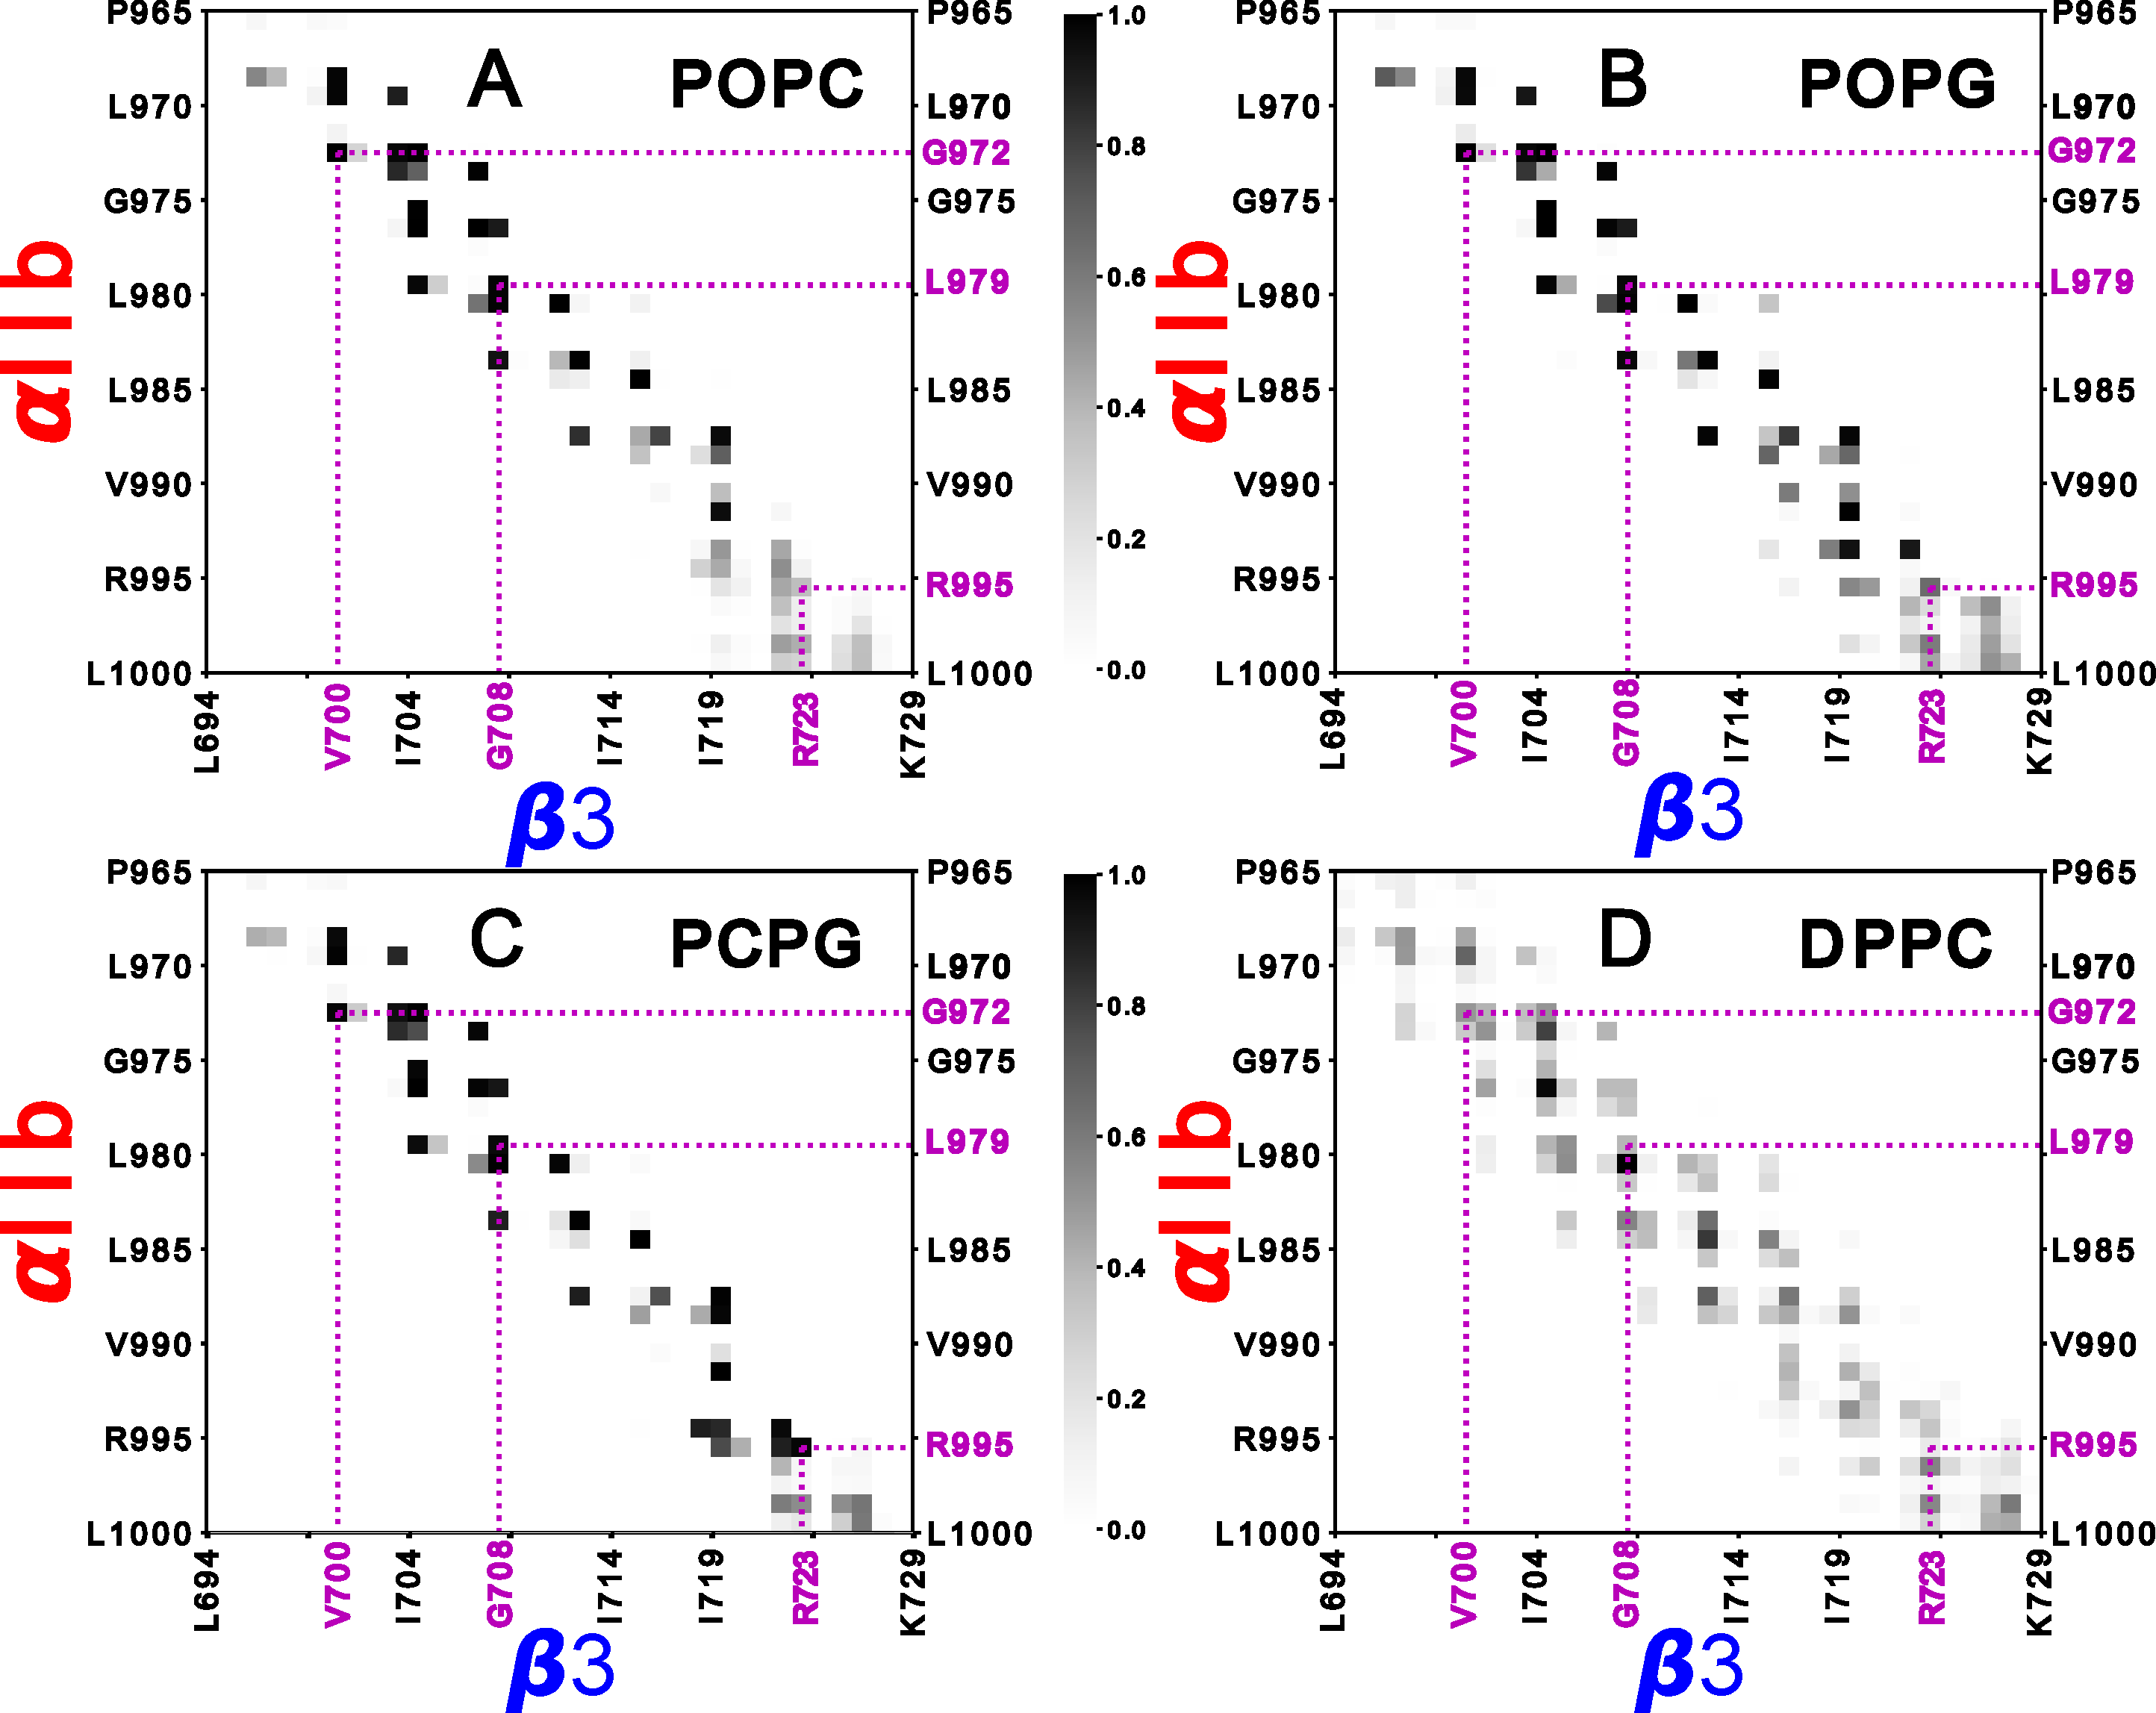
\includegraphics[width=1\linewidth, height=0.8\textheight, keepaspectratio]{fig/02_dm/contact_map2.pdf}
	\caption{Distrubuciónd e densidad de grupos  \textbf{b-c-d)} POPC, DPPC y PCPG}
        \index{headmap}
    	\label{fig:headmap}
\end{figure}

%%%%%%%%%%%%%%%%%%%%%%% Fin %%%%%%%%%%%%%%%%%%%%%%%%



%%%%%%%%%%% Figura %%%%%%%%%%%%
\begin{figure}[H]
    \centering
	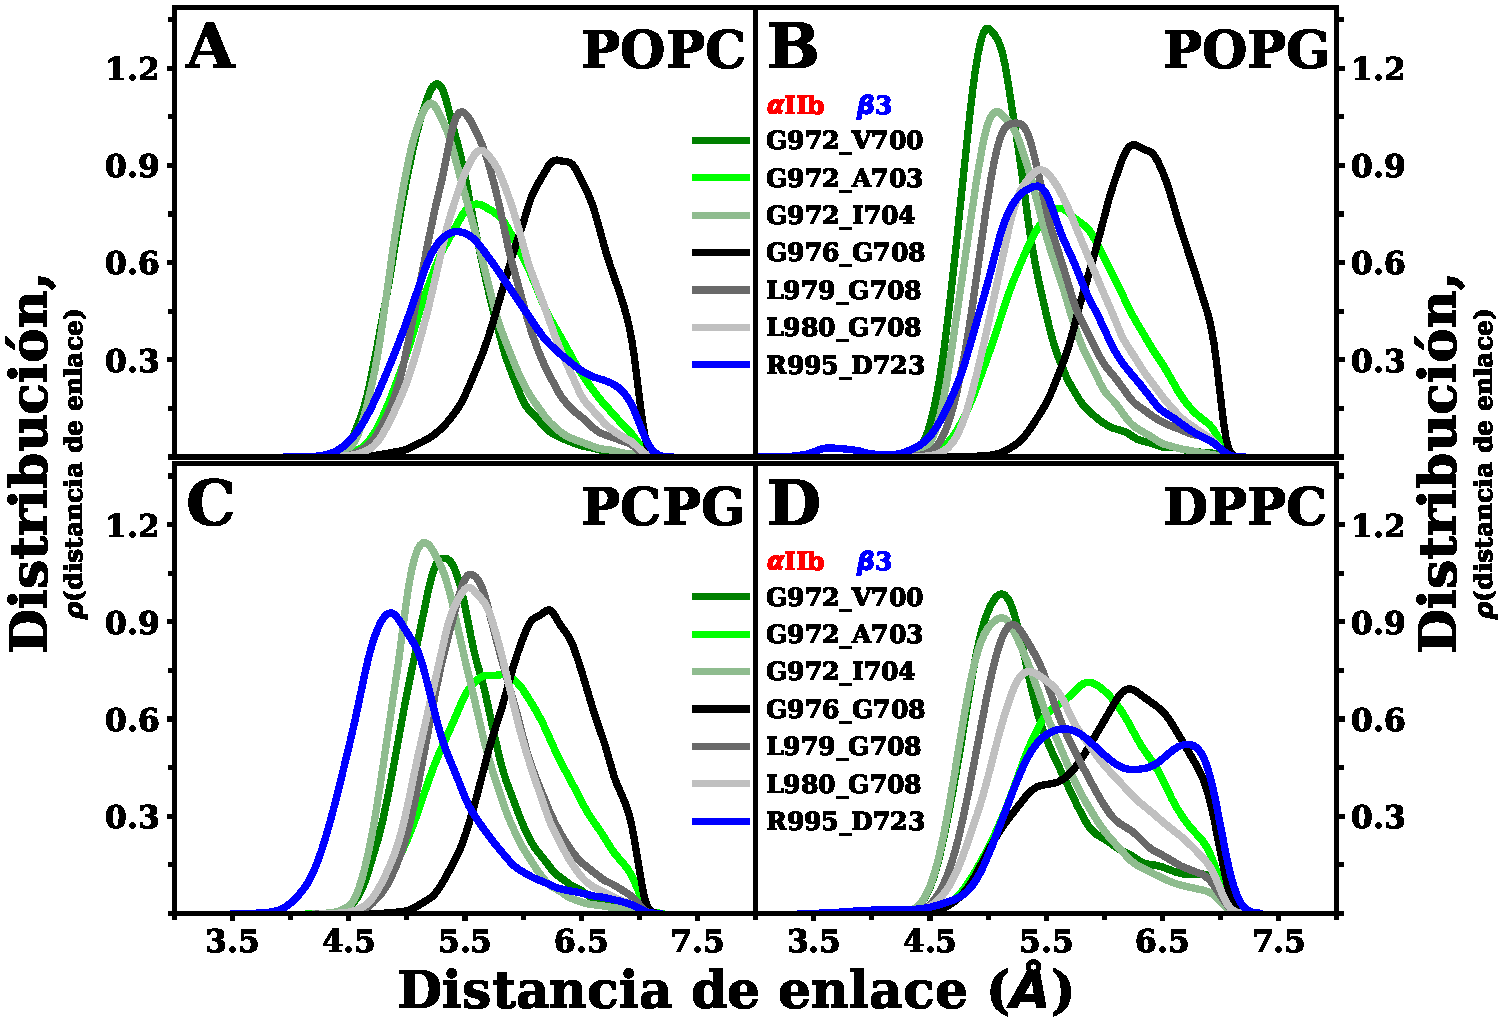
\includegraphics[width=1\linewidth, height=0.99\textheight, keepaspectratio]{fig/02_dm/distance_contacts_all.pdf} 
	\caption{Distribución de densidad de contactos residuos de interés entre heterodímero}
      \index{contac}
    \label{fig:contac}
\end{figure}
%%%%%%%%%%%%%%%%%%%%%%% Fin %%%%%%%%%%%%%%%%%%%%%%%%


%%%%%%%%%%% Figura %%%%%%%%%%%%
\begin{figure}[H]
    \centering
	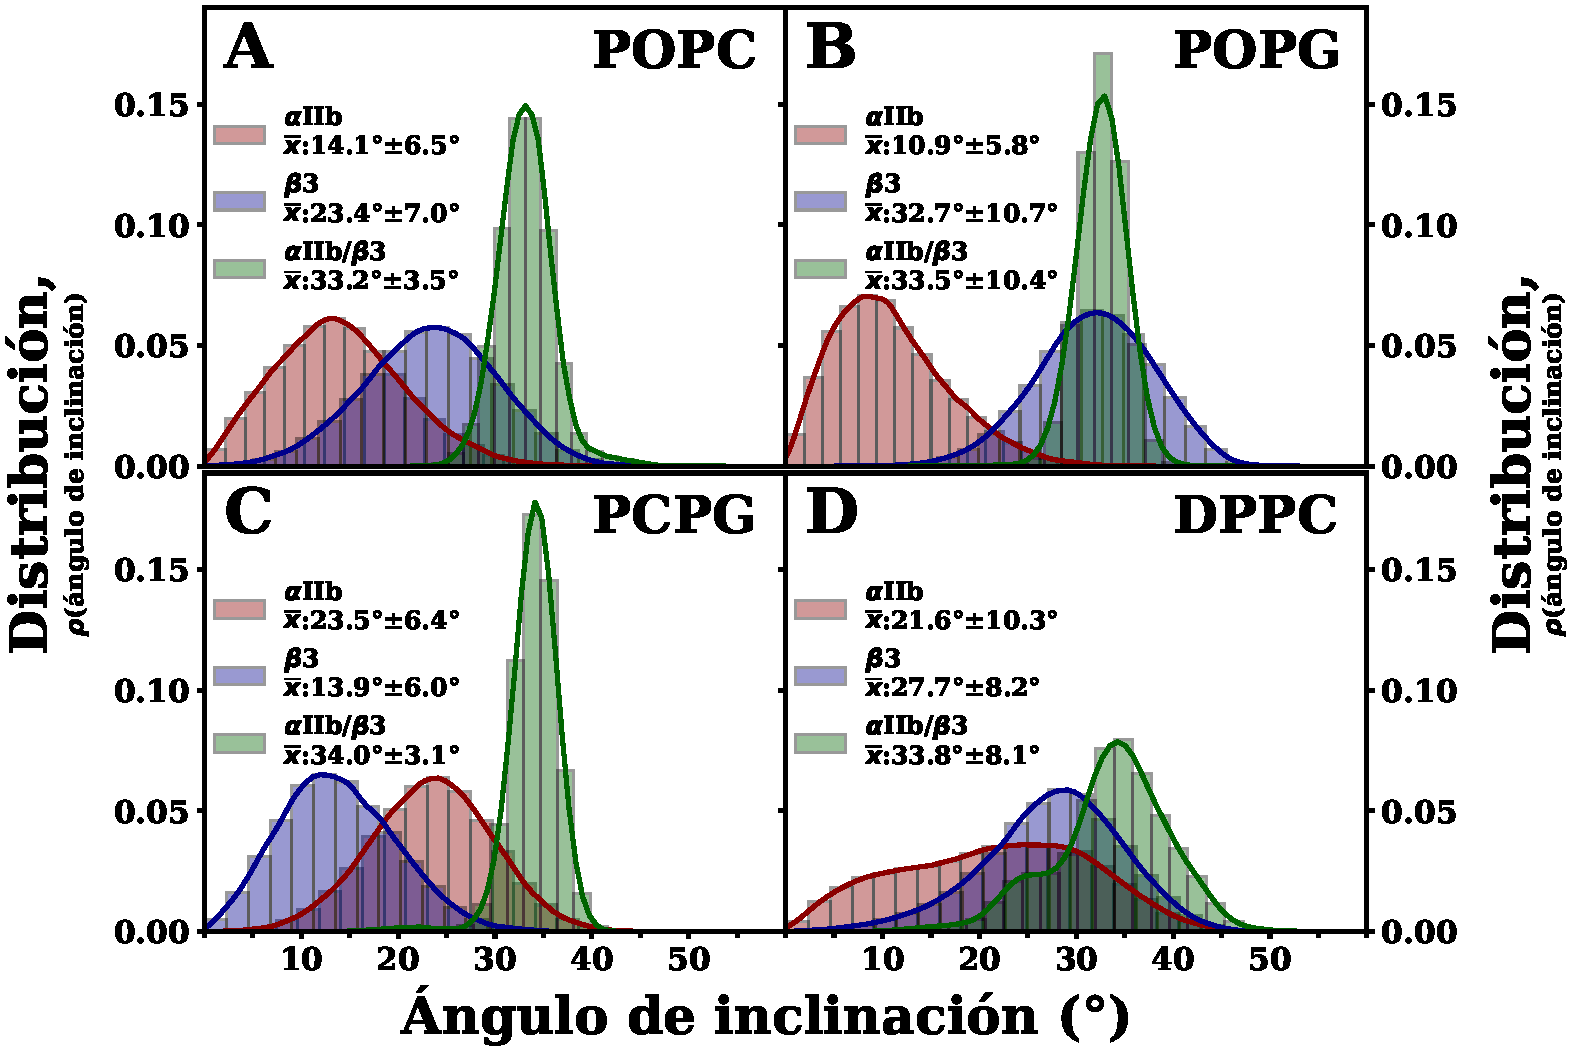
\includegraphics[width=1\linewidth, height=0.8\textheight, keepaspectratio]{fig/02_dm/angles.pdf} 
	\caption[Inclinación respecto a la normal de la bicapa para segmento transmembrana y el ángulo de cruce $\alpha$IIb/$\beta$3]{Inclinación respecto a la normal de la bicapa para segmento transmembrana y el ángulo de cruce $\alpha$IIb/$\beta$3.}
      \index{angles}
    \label{fig:angles}
\end{figure}
%%%%%%%%%%%%%%%%%%%%%%% Fin %%%%%%%%%%%%%%%%%%%%%%%%




%%%%%Tabla resumen membranas%%%%
\begin{table}[h!]
  \begin{center}
%  \centering
%  \captionsetup{justification=centering}  % Center the caption
  \begin{threeparttable}
\centering
    \caption{Área molecular por lípido (APL), parámetro de orden  (S\textbf{\LARGE{$_{cc}$}}) y espesor de membrana durante los 4.5 $\mu$s de simulación. Todos los valores tienen un margen de error de 0.01.}
    \label{tab:parame_lipid}
    \begin{tabular}{l| c c c c}
      \toprule % <-- Toprule here
		Parámetro 					&  POPC	& POPG 	& PCPG 	& DPPC \\ 
      \midrule % <-- Midrule here
		APL (Å\textsuperscript{2}) & 72 	& 73 	& 72 	& 69 \\ 

		S\textbf{\LARGE{$_{cc}$}} 					& 0.52 	& 0.53 	& 0.54	& 0.56 \\ 

		Espesor (Å) 					& 38 	& 34 	& 36 	& 36 \\ 
      \bottomrule % <-- Bottomrule here
    \end{tabular}
    \end{threeparttable}
  \end{center}
\end{table}
%%%%Fin tabla#%%%%%%%%%

%%%%%%%%%%% Figura %%%%%%%%%%%%
\begin{figure}[H]
    \centering
	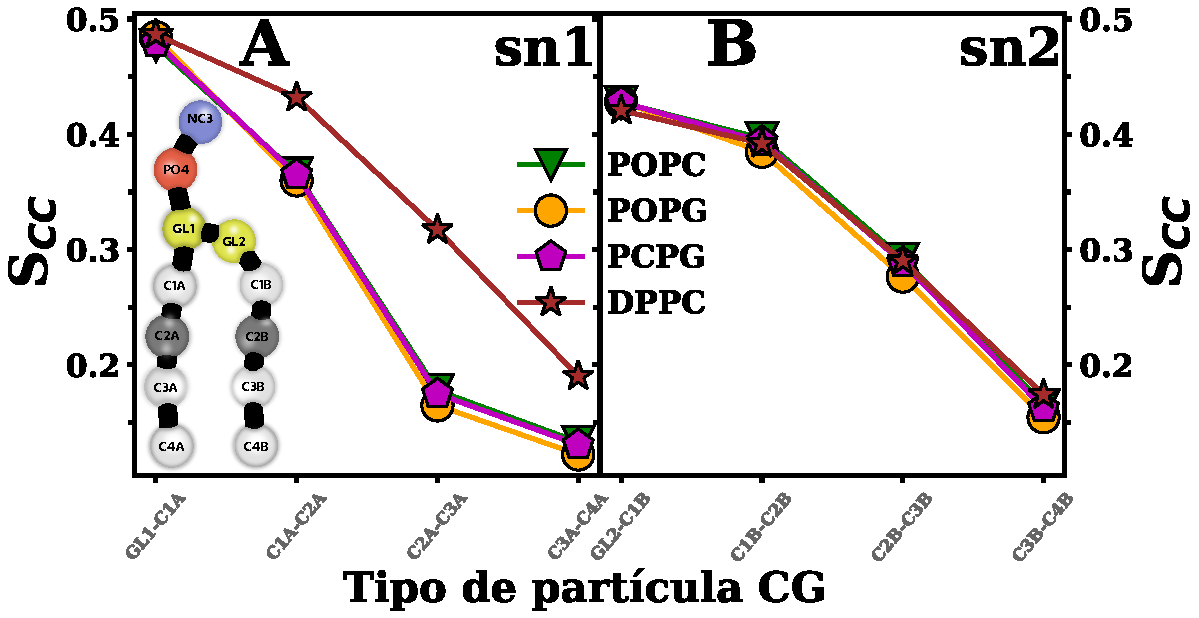
\includegraphics[width=1\linewidth, height=0.99\textheight, keepaspectratio]{fig/02_dm/scc_all.pdf} 
\caption[Parámetro de orden de los lípidos]{Parámetro de orden de los lípidos. Notar que C2A y C2B se resaltan en color diferente porque según el líído que estemos trabajando puede ser D2A y/o D2B}
        \index{areaL}
    \label{fig:scc}
\end{figure}
%%%%%%%%%%%%%%%%%%%%%%% Fin %%%%%%%%%%%%%%%%%%%%%%%%


%%%%%%%%%%% Figura %%%%%%%%%%%%
\begin{figure}[]
    \centering
	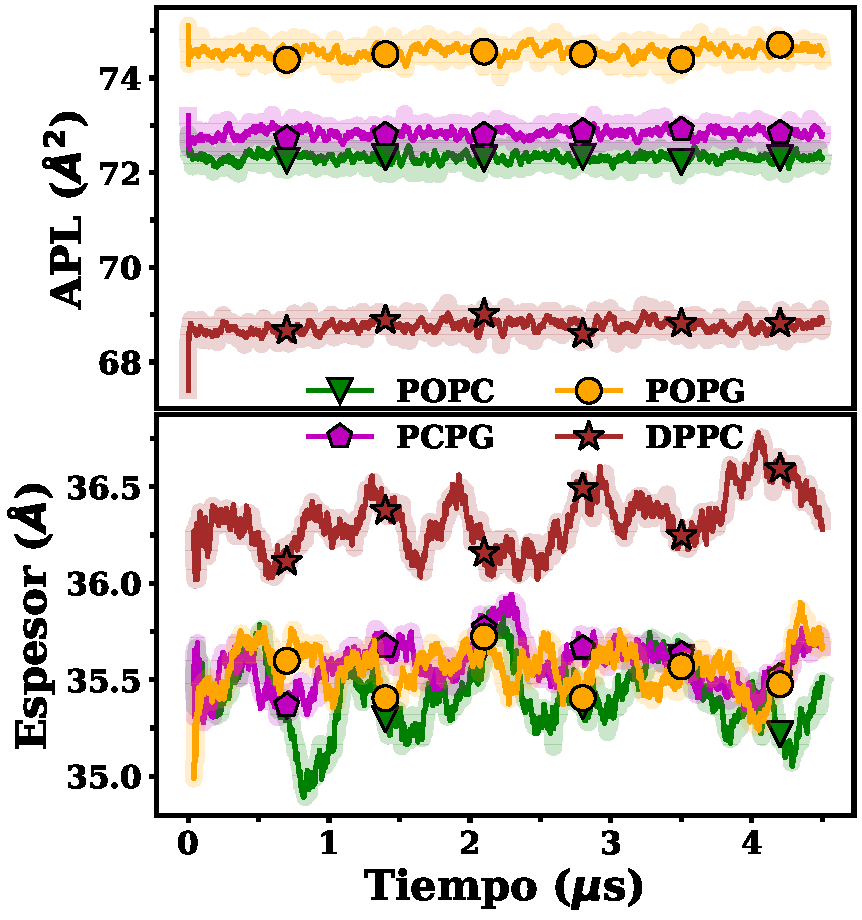
\includegraphics[width=1\linewidth, height=0.99\textheight, keepaspectratio]{fig/02_dm/ApL_zthickness_all.pdf} 
\caption[Área por lípido y espesor de membrana.]{Área por lípido y espesor de membrana.}
        \index{areaL}
    \label{fig:apl_zThick}
\end{figure}
%%%%%%%%%%%%%%%%%%%%%%% Fin %%%%%%%%%%%%%%%%%%%%%%%%


%%%%%%%%%%% Figura %%%%%%%%%%%%
\begin{figure}[H]
    \centering
	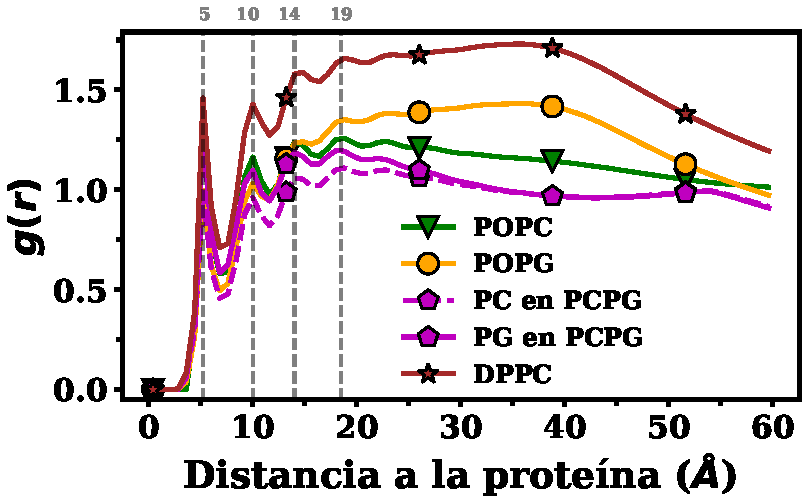
\includegraphics[width=1\linewidth, height=0.99\textheight, keepaspectratio]{fig/02_dm/rdf_all.pdf} 
	\caption[Función de distribución radial] {Función de distribución radial, g(r) para los lípidos respecto al heterodímero $\alpha$IIb/$\beta$3.}
      \index{rdf}
    \label{fig:rdf}
\end{figure}
%%%%%%%%%%%%%%%%%%%%%%% Fin %%%%%%%%%%%%%%%%%%%%%%%%



\begin{table}[H]
\begin{center}
  \begin{threeparttable}
\centering
    \caption[Número de lípidos en contacto con los péptidos.]{Número de lípidos en contacto con los péptidos. Como criterio de contacto se usó un  \textit{cutoff} de 6.0 Å entre el grupo polar PO4 y el centro de masa de los residuos en cada péptido.}
    \label{tab:lipid_pept_contac}
\begin{tabular}{@{}ccccc@{}}
\toprule
                                   & \textbf{POPC}                 & \textbf{POPG}                 & \textbf{PCPG}                 & \textbf{DPPC}                 \\ \cmidrule(l){2-5} 
\multirow{-2}{*}{Péptido} &
  $\overline{x}$\textpm std &
  $\overline{x}$\textpm std &
  $\overline{x}$\textpm std &
  $\overline{x}$\textpm std \\ \midrule
{\color[HTML]{FE0000} $\alpha$IIb} & 19.8\textpm4.8 & 12.1\textpm4.5 & 16.9\textpm5.4 & 13.8\textpm5.3 \\ 
{\color[HTML]{3531FF} $\beta$3}    & 11.1\textpm3.9 & 1.4\textpm4.0  & 13.9\textpm5.4 & 0.9\textpm2.5  \\ \bottomrule
\end{tabular}
\end{threeparttable}
\end{center}
\end{table}



%%%%%%%%%%% Figura %%%%%%%%%%%%
\begin{figure}[H]
    \centering
	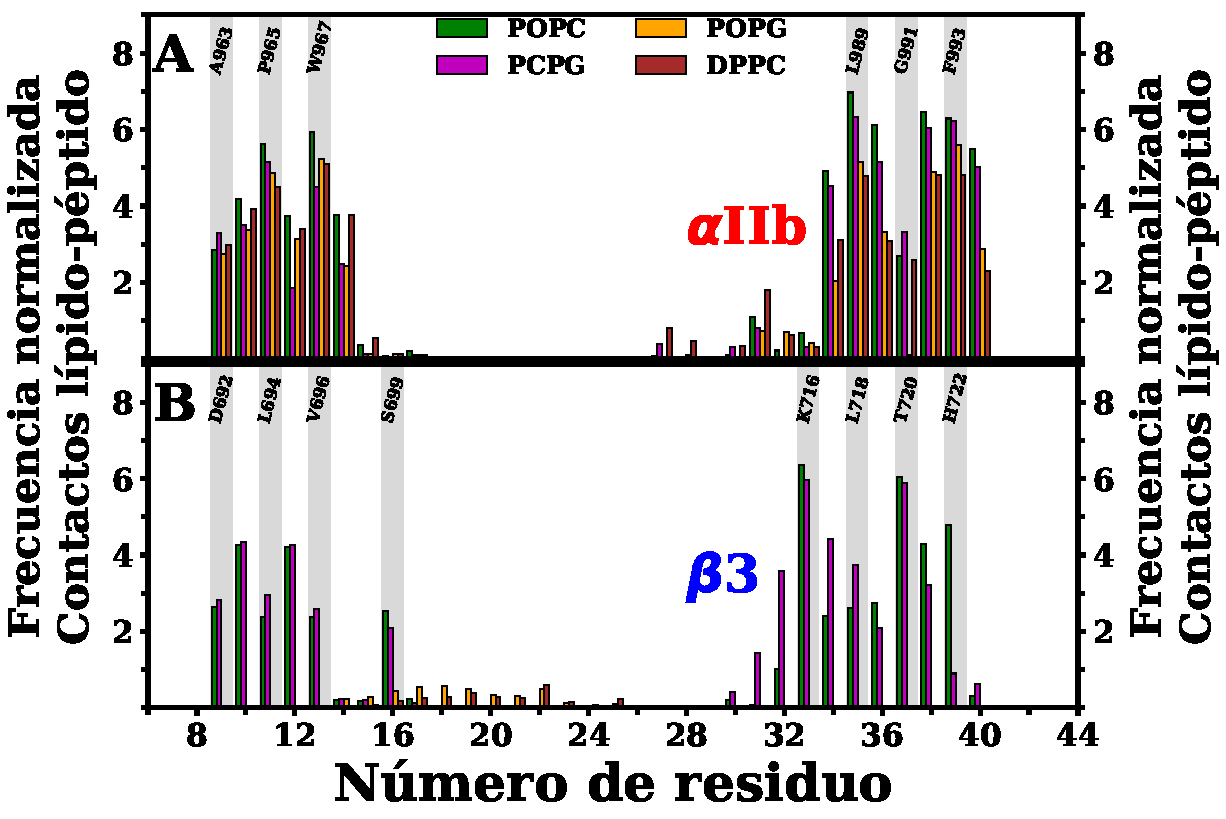
\includegraphics[width=1\linewidth, height=0.99\textheight, keepaspectratio]{fig/02_dm/lipid_pept_contac_all.pdf} 
	\caption[Frecuencia de contactos lípido-residuos durante la dinámica.]{Frecuencia de contactos lípido-residuos durante la dinámica}
      \index{lipid_resid_contact}
    \label{fig:lipid_resID_contac}
\end{figure}
%%%%%%%%%%%%%%%%%%%%%%% Fin %%%%%%%%%%%%%%%%%%%%%%%%
%\chapter{Cap\'{\i}tulo ...}
Se deben incluir tantos cap\'{\i}tulos como se requieran; sin embargo, se recomienda que la tesis  o trabajo de investigaci\'{o}n tenga un m\'{\i}nimo 3 cap\'{\i}tulos y m\'{a}ximo de 6 cap\'{\i}tulos (incluyendo las conclusiones).\\
\chapter{Conclusiones y recomendaciones}
\section{Conclusiones}
Las conclusiones constituyen un cap\'{\i}tulo independiente y presentan, en forma l\'{o}gica, los resultados de la tesis  o trabajo de investigaci\'{o}n. Las conclusiones deben ser la respuesta a los objetivos o prop\'{o}sitos planteados. Se deben titular con la palabra conclusiones en el mismo formato de los t\'{\i}tulos de los cap\'{\i}tulos anteriores (T\'{\i}tulos primer nivel), precedida por el numeral correspondiente (seg\'{u}n la presente plantilla).\\

\section{Recomendaciones}
Se presentan como una serie de aspectos que se podr\'{\i}an realizar en un futuro para emprender investigaciones similares o fortalecer la investigaci\'{o}n realizada. Deben contemplar las perspectivas de la investigaci\'{o}n, las cuales son sugerencias, proyecciones o alternativas que se presentan para modificar, cambiar o incidir sobre una situaci\'{o}n espec\'{\i}fica o una problem\'{a}tica encontrada. Pueden presentarse como un texto con caracter\'{\i}sticas argumentativas, resultado de una reflexi\'{o}n acerca de la tesis o trabajo de investigaci\'{o}n.\\
\begin{appendix}

\chapter{Protocolo extracción y clonación de plásmidos}\label{Protocolo Plasmido}

Los plásmidos gentilmente donados por el laboratorio del Dr. Qin, fueron depositados en una gota sobre un papel y resaltado el contorno en circunferencia rotulada cada uno como $\alpha$IIb y $\beta$3, a partir de éstos se procedió con la extracción y clonación de cada uno por separado.


\begin{table}[]
  \begin{center}
  \centering
  \captionsetup{justification=centering}  % Center the caption
    \caption{Datos proteína fusión, segmentos transmembrana, MBP y TEV.}
    \label{tab:dat_proteina}
    \begin{tabular}{l l| l l }
      \toprule % <-- Toprule here

		$\alpha$IIb-Fusión & 49.41 kDa 	& $\alpha$IIb 	& 6.05 kDa \\ 
		{\Large{$\varepsilon$}}$_{\alpha \text{IIb-Fusión}}$ & 85830 M$^{\text{-1}}$cm$^{\text{-1}}$ & {\Large{$\varepsilon$}}$_{\alpha \text{IIb}}$ & 16500 M$^{\text{-1}}$cm$^{\text{-1}}$ \\
		$\beta$3-Fusión 	& 52.11 kDa 	& $\beta$3 	& 8.76 kDa \\
		{\Large{$\varepsilon$}}$_{\beta \text{3-Fusión}}$ & 83310 M$^{\text{-1}}$cm$^{\text{-1}}$ & {\Large{$\varepsilon$}}$_{\beta \text{3}}$ & 13980 M$^{\text{-1}}$cm$^{\text{-1}}$ \\
      \midrule % <-- Midrule here
      MPB & 42.49 kDa 	& TEV 	& 28.62 kDa \\ 
      
      
      \bottomrule % <-- Bottomrule here
    \end{tabular}
  \end{center}
\end{table}



    \begin{itemize}
     
     \item{Suspensión del plásmido en Buffer Trix}
      \begin{itemize}
        \item{Recortar media circunferencia de cada plásmido (tijeras estériles, limpiar con alcohol y flamear en fuego)}
        \item{Guardar el otro pedazo de papel a -20°C en bolsa ziploc}
        \item{Manipular con al semi-circunferencia con unas pinzas estériles, cortarlo en pedazos más pequeños}
        \item{Introducir los pedacitos en un eppendorf rotulado como corresponde ($\alpha$IIb ó $\beta$3)}
        \item{Agregar 50 µL de buffer Trix 50 mM pH 8. Evitar diluir mucho el plásmido}
        \item{Dejar 30 minutos en suspensión}
      \end{itemize}
    
    \item{Clonar los plásmidos}
      \begin{itemize}
        \item{Rotular dos viales eppendorf según corresponda, dejarlos en hielo}
        \item{Agregar a cada vial 100 µL de la cepa \emph{E. coli} DH5$\alpha$}
        \item{Tomar 10 µL del plásmido re-suspendido y transferirlos al vial que contiene la bacteria \emph{E. coli} DH5$\alpha$}
        \item{Tapar y dejar durante 30 minutos en hielo. Mientras espera, calentar baño termostático a 42°C}
        \item{Pasada la media hora, colocar los viales en el baño caliente durante 1 minuto y 30 segundos. Usar flotador de eppendorf}
        \item{Colocar de nuevo en el hielo durante 5 minutos}
        \item{Preparar el LB,  agregar 900 µL de LB a los eppendorf de $\alpha$IIb y $\beta$3 que contienen 100 $\mu$L de la cepa E. coli DH5$\alpha$ y los 10 µL de la suspensión de plásmido}
        \item{Llevarlos a 37°C durante 1 hora}
    \end{itemize}
    
    \item{Cultivo en caja de Petri}

     Utilizar 4 tubos ro, dos para el $\alpha$IIb y dos para el $\beta$3, donde tendremos una siembra diluida y una concentrada, es decir, de los tubos eppendorf anteriores (que contienen 900 $\mu$L de LB, 100 µL de la cepa E. coli DH5$\alpha$ y los 10 µL de la suspensión de cada plásmido), que tenemos después de someter a 37 °C durante una hora, ese líquido en primera instancia lo llamaremos “células diluidas”, luego centrifugamos a 4000 rpm/5 min (se va a observar un precipitado) y pipeteamos con mucho cuidado 800 $\mu$L los cuales desecharemos. Luego vamos a resuspender ese precipitado pipeteando lentamente y esa serán las “células concentradas”.

     \begin{itemize}
        \item{}
        \item{}
        \item{}
        \item{}
    \end{itemize}
        

Para el sembrado debemos tener las 4 cajas de Petri rotuladas como corresponde (diluida y concentrada tanto para $\alpha$IIb como $\beta$3). Utilizar perlas pequeñas para facilitar la “dispersión” de las células en el cultivo, para ello usar una “cucharita” que se flamea antes de sacar las perlas (entre 4 a 6 perlitas por caja de Petri). Evitar que las perlitas giren en círculos sobre las paredes de las cajas de Petri, la idea es que recorran todo el medio y no solo las paredes del medio.

Pipetear 100 µL de “células” y depositarlos sobre las perlitas, luego tapar la caja y agitar con la finalidad que se “depositen” células por todo el medio y obtener diferentes colonias de bacterias que se puedan aislar fácilmente. 


\item{Aislamiento de colonias}

De los cultivos que obtuvo anteriormente, seleccionar los que permitan aislar y/o identificar fácilmente una colonia. Las cuales se van a sembrar nuevamente en una caja de Petri con el mismo medio (LB con ampicilina 100 µg/mL; previamente secar). Para el caso específico se obtuvieron muchas colonias en las concentradas y se dificulta identificar algunas colonias, por lo tanto, seleccionamos las “diluidas” las cuales tenían colonias separadas unas de otras lo cual permite que “puncemos” con un palillo una colonia y luego sembrarla en el nuevo medio para aislar, y en medio de LB líquidos los cuales se guardarán en un freezer a -80 °C, más adelante. 
Sobre la tapa de los cultivos que mejor permite identificar colonias, encerrar cuatro colonias que son las que va a punzar con el palillo y posteriormente sembrar en el nuevo medio de cultivo.

     \begin{itemize}
        \item{}
        \item{}
        \item{}
        \item{}
    \end{itemize}


Además, los palillos que se usan en $\alpha$IIb$_{1,2}$ y $\beta$3$_{1,2}$ se introducen en los medios líquidos de LB, cada tubo de ensayo debe contener 2.5 mL LB con ampicilina [100 µg/mL]. Los palillos 3 y 4 se pueden desechar. La caja de Petri se incuba a 37 °C por más de 12 horas y los tubos de ensayo, con sus respectivas tapas se llevan a shaker a 37 °C por más de 12 horas.

NOTAS: 
    A. La idea de sembrar nuevamente en LB sólido es porque se obtienen colonias aisladas y una vez crezcan son las que se utilizarán para extraer los plásmidos y sembrarlos nuevamente, pero en la cepa de expresión.
    B. Los cultivos líquidos se hacen con la idea de que una vez se obtengan las células, se dejan en una solución de glicerol al 15$\%$ a -80 °C, y se usarán como “solución stock” cuando se necesite obtener células con el plásmido para expresar.

    C. Las cajas de los primeros 4 cultivos se guardan temporalmente en una nevera para tenerlas como respaldo por si pasa algo. 
    D. Para la preparación del LB con ampicilina, se debe solicitar a FACEMES el antibiótico, ellos entregan un eppendorf con 500 µL a una concentración de [100 mg/mL], el cual debe conservar siempre en hielo y dejar que se descongele en el hielo y una vez termine de usarlo, guardarlo a -20°C. El LB que se usa, es un frasco que viene rotulado como LB 50 mL; sino lo va usar todo procure preparar la cantidad necesaria y guardar bien el resto de LB sin antibiótico, ejemplo, si sólo necesita 20 mL de LB, y sabemos que la concentración de ampicilina debe ser [100 $\mu$g/mL], entonces le agregamos 20 $\mu$L de los 500 $\mu$L que le entrega FACEMES. 


\item{Guardar células en glicerol al 15$\%$ a -80°C}

De cada tubo de ensayo de cultivo líquido de LB, se extraen 500 µL y se vierten un tubo eppendorf, previamente rotulado y luego se le agredan 500 µL de glicerol al 30$\%$, es decir se obtiene 1 mL de “solución \textbf{stock de células}” al 15$\%$ de glicerol. Además, cada tubo se debe hacer por duplicado, y éstas son las muestras que se guardan a -80 °C. 
Antes de pipetear los 500 µL de células agitar bien el tubo y cuando agregue el glicerol, con la misma punta pipetear suave para que se “disuelva” bien el glicerol la solución.
Procurar tener todos los eppendorf tapados e ir trabajando uno por una por si de pronto salpica alguna gota de una cepa a un tubo diferente.

     \begin{itemize}
        \item{}
        \item{}
        \item{}
        \item{}
    \end{itemize}



\item{Minipreps y test de pureza}

Extracción de los plásmidos (Plus SV Minipreps DNA Purification System-Quick Protocol)
    A. Production of Cleared Lysate
De los cultivos del paso anterior, agitarlos un poco antes de pipetear de cada uno 1.5 mL y agregarlos en eppendorf rotulados como corresponde y dejar 5 minutos quieto. Al centrifugar colocar de la misma forma los tubos para que el pellet se forme siempre en el mismo lado de los tubos. Esto se hace porque en ocasiones el pellet no se ve a simple vista y si siempre colocamos los tubos de la misma forma, se sabrá en donde se encuentra y así uno cuando succione con la punta sabe que no debe tocar esa zona donde se supone que el pellet.

Cuando termine de centrifugar extraer de cada tubo la máxima cantidad posible del sobrenadante de cada tubo SIN TOCAR el pellet. Cambiar de punta cada vez que cambia de cepa. El sobrenadante se puede desechar. Aquí lo que se hace es obtener todas las células que contienen el plásmido.

Al terminar deberá obtener 4 tubos eppendorf con los correspondientes pellets, dos se guardan a -20 °C para tenerlos de respaldo por si algo o no se logra extraer el plásmido se parte de nuevo, pero de esas dos muestras que se guardan.
Se continua con el punto 2 del protocolo. Donde a los dos tubos se les agrega 250 mL de “Cell Resuspension Solution”. Tener mucho cuidado al pipetear de esta y las otras soluciones del protocolo, es decir, si al verter los 250 µL en uno de los tubos llega a tocar las paredes del mismo DEBE descartar esa punta y usar otra para pipetear de nuevo el reactivo correspondiente.

Una vez termine de agregar la solución de Resuspención, llevar cada tubo al vortex con la idea de que todo el pellet se disuelva; si necesita golpearlo con los dedos lo puede hacer. Observar que la solución que se obtiene es un poco “turbia” 

Punto 3: agregar 250 µL de “Cell Lysis Solution” a cada tubo e inmediatamente “invertir” el tubo suavemente unas 5-6 veces; debe observarse un cambio en la coloración, pasa de blanco-turbia a traslúcida. Lo que se hace en este paso es romper todas las células y sale el ADN que le da una “viscosidad” a la solución. Procurar no tener tanto tiempo en la mano el tubo después de agregar la solución de lisis.
Punto 4: Agregar 10 µL de “Alkaline Protease Solution”; en este caso como es una pequeña cantidad de solución, tratar de que con la misma punta que pipeteó los 10 µL, al agregarlos dentro de la solución y desechar la punta. Dejar 5 minutos en una gradilla a temperatura ambiente. Al agregar esta solución lo que se está haciendo es “desnaturalizar el ADN junto con las proteínas.
Punto 5: Agregar 350 µL de “Neutralization Solution”, casi que de inmediato se van a forman “grumos” blancos lo cual indica que se han “renaturalizado” proteínas, el ADN plasmático queda en la solución. 
Punto 6: Centrifugar a 13 mil rpm durante 10 minutos a 25 °C. 
Es muy importante no pipetear partes blancas; puede colocar dos puntas en la micropipeta para que se facilite y succione mejor el líquido. El eppendorf de donde sacamos el líquido, se desecha en una bolsa roja. 

    B. Binding of Plasmid DNA
Punto 7-8: El líquido que se pipetea se vierte en la columna o tubo de membrana “Spin Column” con su correspondiente tubo colector (puede ser un eppendorf estéril.
Punto 9: Centrifugar por un minuto a 13 mil rpm a temperatura ambiente. El contenido del líquido del tubo colector se descarta. Tener mucho cuidado al retirar la Spin Column de no tocar las paredes internas y mucho menos la membrana.
    C. Washing
Punto 10: Para el lavado se agregan 750 µL de “Wash Solution” 

Paso extra!!
Antes de la elución cambiar el tubo colector y colocar la Spin Column en otro tubo colector que esté limpio, seco y sin EtOH o puede usar un eppendorf y soportar la Spin Column en este y centrifugar así sin nada por 2 minutos a 13 mil rpm. La idea es que no quede nada de EtOH en la columna.

    D. Elution
Lo que se hará en éste paso es desprender el plásmido que quedó en la membrana, por lo tanto, se debe buscar un eppendorf totalmente estéril y nuevo, los cuales deben estar rotulados como corresponde. 
Punto 13: Transferimos la Spin Column como se hizo en el paso extra.
Punto 14: Agregar 100 µL de “Nuclease-Free Water” o la mejor calidad de agua ultra pura que tenga. Procurar en este paso verter el agua cerca de la membrana, pero sin tocarla y desechar la punta que se usó. Dejar 2 minutos en reposo como para que se absorba bien el agua y luego centrifugar a 13 mil rpm por 1 minuto con la tapa abierta.


     \begin{itemize}
        \item{}
        \item{}
        \item{}
        \item{}
    \end{itemize}
\end{itemize}

\chapter{Protocolo expresión, lisis y purificación de proteína fusión}\label{Protocolo_Fusion}
El siguiente protocolo se realizó para expresar 4L de cultivo de proteína fusión a partir del stock\textbf{stock de células} de cada péptido.

\subsection{Expresión}

\begin{itemize}
    \item{Pre-inóculo en cepa \ac{ecoli} BL21(DE3)}
    \begin{itemize}
        \item{Tomar un frasco de agar \ac{lb} de 100 mL}
        \item{Suplementar con 100 µL de ampicilina stock [100 mg/mL]}
        \item{Sacar uno de los \textbf{stock de células} en hielo}
        \item{Usar punta (tip) amarillo para raspar y sacar células y arrojar tips al frasco}
        \item{Dejar overnight a 37°C toda la noche con agitación constante}
    \end{itemize}

    \item{Crecer células e inducir con IPTG}.
    Para crecer las células se usaron Erlenmeyers de capacidad para 3L pero se agregaron 1L de \ac{lb} en cada uno suplementado con 1.0 mL de ampicilina [100 mg/mL].
    \begin{itemize}
        \item{Tomar 25 mL del precultivo y agregarlo a cada Erlenmeyer}
        \item{Crecer a 37°C con agitación constante hasta obtener una \ac{DO$_{600}$} entre 0.7-0.8 ($\approx$ 7 horas)}
        \item{Agregar 1.0 mL de IPTG 1 M, [1.0 mM]$_{final}$}
        \item{Fortificar ampicilina, agregando 500 µL a cada cultivo}
        \item{Dejar nuevamente a 37°C con agitación por 5 horas}
    \end{itemize}

        \item{Centrifugar medios}
    \begin{itemize}
        \item{Trasvasar el cultivo a los frasco de polipropileno Nalgene (capacidad de 500 mL). Verificar que todas tengan el mismo peso}
        \item{Colectar células por centrifugación a 4°C, 4500 \ac{rpm} durante 30 minutos}
        \item{Descartar el sobrenadante}
    \end{itemize}
    Después de obtener un \textbf{pellet} (precipitado) en cada frasco, juntar en 2 falcón de 50 mL y guardar a -20°C si va lisar pronto, de lo contrario guardar a -80°C, congelando previamente con nitrógeno líquido.
\end{itemize}

\section{Lisis de células}
Seguimiendo de la proteína por geles de \ac{SDS-PAGE}, parte de la proteína fusión fue a cuerpos de inclusión, por lo tanto, para obtener la mayor cantidad de proteína se realizó un rompimiento de células exhaustivo aplicando tres métodos de lisis: ciclos frío-calor, incubación con Lisozima-ADNasa, (Freeze/Thaw) y alta presión (homogeneizador Emulsiflex).


\begin{itemize}
\item{Ciclos frío-calor}
     \begin{itemize}
         \item{Resuspender cada pellet en 25 mL buffer de lisis \ac{pbs} 20 mM, 300 mM NaCl y 20 mM imidazol} + Triton X-100 [0.25$\%$]$_{final}$ (v/v)
        \item{Congelar muestras con nitrógeno líquido y dejar a -80°C por 2 horas}
        \item{Descongelar en un baño de agua a temperatura ambiente}
        \item{Repetir proceso al menos 3 veces}
    \end{itemize}
\end{itemize}

\begin{itemize}
\item{incubación con Lisozima-ADNasa}
     \begin{itemize}
        \item{Agregar inhibidor de proteasa \ac{pmsf} a concentración [1 mM]$_{final}$}
        \item{Agregar lisozima bovina [5 mg/L cultivo]$_{final}$}
        \item{Agregar DNAsa [0.5 mg/L cultivo]$_{final}$}
        \item{Agregar EDTA [1.0 mM]$_{final}$}
        \item{Dejar a 4°C con agitación en rotor overnight}
    \end{itemize}
\end{itemize}

\begin{itemize}
\item{Homogeneizador Emulsiflex}
     \begin{itemize}
        \item{Pasar cada muestra al menos 4 veces por el Emulsiflex}
        \item{Fijarse visualmente en la densidad y flujo al salir del Emulsiflex}
        \item{Después de los 4 ciclos, la muestra debe ser casi un líquido fluido}
    \end{itemize}

Finalmente las muestras fueron centrifudas a 9500 \ac{rpm} por 30 minutos a 4°C (Eppendorf™ Centrifuge 5804R), conservando el \textbf{sobrenadante}. 
\end{itemize}

\section{Purificación por \ac{fplc}}

\begin{itemize}
    \item{Elución}
     \begin{itemize}
        \item{Equilibrar la columna con buffer A (el mismo de lisis)}
        \item{Cargar el contenido de 2L de cultivo; si carga más podría sobre saturar la columna. Usar bomba peristáltica}
        \item{Lavar con 10 \ac{cv} pasando buffer A. NO DESCARTAR ya que por geles \ac{SDS-PAGE} se observó que había proteína fusión, por lo tanto, se pasó después nuevamente por la columna}
        \item{Llevar columna al \"{A}KTA y pasar otros 10-20 mL de buffer A para obtener una buena base de linea en el cromatograma}
        \item{Eluir con buffer B, gradiente de imidazol de 20 a 400 mM (\ac{pbs} 20 mM, NaCl 300 mM, 400 mM imizadol)}
        \item{Colectar fracciones}
    \end{itemize}
\end{itemize}

\section{Concentrar y desalar proteína fusión}
Antes de cuantificar la concentración de cada proteína fusión, se procedió a concentrar todo el contenido de las fracciones colectadas en centricones Amicon Ultra-15 Centrifugal con 30 kDa  cutoff y cambiar de buffer en columnas PD-10 Desalting (GE Healthcare).

\begin{itemize}
    \item{Concentrar}
     \begin{itemize}
        \item{Lavar centricones de cuttoff 30 kDa agua Milli-Q}
        \item{Juntar todas las fracciones colectadas}
        \item{Agregar igual cantidad de volumen a cada Amicon}
        \item{Centrifugar a 4500 \ac{rpm} a 4°C por $\approx$ 20 minutos}
        \item{Conservar el contenido retenido}
        \item{Repetir pasos hasta concentrar toda la muestra}
    \end{itemize}

    \item{Desalar}
     \begin{itemize}
        \item{Equilibrar columna con buffer C (\ac{pbs} 20 mM, NaCl 150 mM y 7.5$\%$ glicerol (vol/vol) pH 7.4)}
        \item{Cargar muestra y eluir hasta casi sequedad}
        \item{Agregar buffer C, eluir}
        \item{Repetir hasta pasar toda la muestra previamente concentrada}
    \end{itemize}
    \item{Cuantificar por  espectrofotometría \ac{uv}}
    \item{Fraccionar en eppendorff y guardar a -20ºC/-80ºC}
Para más detalles consultar la ficha técnica en el siguiente link:  \url{https://www.scientificlabs.co.uk/handlers/libraryFiles.ashx?filename=Manuals_1_17085101_A.pdf}
\end{itemize}

\section{Protocolo de clivaje y diálisis}\label{Protocolo_TEV}

Tener en cuenta que la relación \ac{tev}:proteína es 1:30 mol a mol, por lo tanto, calcular bien la cantidad proteasa a usar según las concentraciones de TEV - proteína.

Ejemplo, si TEV = [1.0 mg/mL] y proteína [1.0 mg/mL], entonces,

$
\left( \frac{1.0 \, mg}{mL}*\frac{1 \,  g}{1000 \, mg}*\frac{1\,  mol\,  \alpha IIb}{49400\,  g}*1 \, mL \right)*10^9= 20.24 \;nmoles \;  \alpha IIb
$


$
\frac{20.24}{30} = 0.67
$

$
0.67\, nmol \,TEV*\frac{1 \,mol}{10^9 \,nmol}*\frac{28619.5 \,g}{1 \,mol\, TEV}*\frac{1000 \,mg}{1 \,g}*\frac{1000\, \mu L}{1\, mL} = 19.17 \; \mu L 
$
\begin{itemize}
    \item{Clivaje con TEV}
    \begin{itemize}
        \item{Descongelar las muestras de proteína}
        \item{Agregar \ac{dtt} [1.0 mM]$_{final}$}
        \item{Agregar 19.17 µL de TEV a cada vial}
        \item{Tapar y agitar suave}
        \item{Dejar a 30ºC por al menos 48 horas}
        \item{Centrifugar todos los viales a 13 mil \ac{rpm} por 10 minutos a temperatura ambiente}
        \item{Recuperar el \textbf{sobrenadante}}
        \item{Juntar todos los sobrenadantes y }
        \item{Concentrar en   Amicon Ultra-15 Centrifugal con 3 kDa  cutoff, 4500 \ac{rpm} a 4°C por $\approx$ 40 minutos}
    \end{itemize}

    \item{Diálisis}
    \begin{itemize}
        \item{Lavar las membranas con EDTA y bicarbonato de sodio a 60ºC por 5 minutos}
        \item{Pasar flujo de agua Milli-Q por la membrana o dejar en remojo con agitación suave por 2 horas}
        \item{Cerrar uno de los estremos, verificar que este bien sellado}
        \item{Agregar la muestra evitando dejar aire pero lo suficiente para sellar el otro extremo}
        \item{Colocar membranas en beaker de al menos 1L con agua Milli-Q
        }
        \item{Dejar 4ºC con agitación suave. Realizar dos cambios de agua al menos dos veces cada 8 horas}
        \item{Remover toda la muestra incluyendo el precipitado y pasarlo a eppendorf}
        \item{Centrifugar todos los viales a 13 mil \ac{rpm} por 10 minutos a temperatura ambiente}
        \item{Separar cuidadosamente el \textbf{pellet}}
        \item{Juntar los pellets en falcón de 50 mL y resuspender en buffer (fase móvil A (H$_{2}$O:\ac{acn} 60\%/\%40, vol/vol, \ac{tfa} 0.01\% vol/vol)}
        \item{Calentar a baño María $\approx$ 40°C para facilitar la solubilización}
        \item{Fraccionar en eppendorf y centrifugar todos los viales a 13 mil \ac{rpm} por 20 minutos a temperatura ambiente}
        \item{Tomar sobrenadante, juntar nuevamente y filtrar con membranas PVDF 0.45 µm (Durapore Merck). Esto para proteger al máximo la columna del \ac{hplc}}
    \end{itemize}

    
\end{itemize}


\chapter{Protocolo \ac{hplc}}\label{Protocolo_HPLC}
Tenga presente que los solventes deben ser grado \ac{hplc}, el agua Milli-Q se debe filtrar con membranas PVDF 0.22 µm y desgasificar. Se recomienda seguir los cuidados de la columna según el manul del usuario disponible en: \url{https://vneshbiotorg.ru/upload/welch/use-and-maintainance-of-hplc-column-welch%20materials.pdf}.

\begin{itemize}
    \item{Purgar equipo y equilibrar columna}
     \begin{itemize}
        \item{Lavar y purgar bombas y loop del  \ac{hplc} con agua y luego con la fase móvil A}
        \item{Equilibrar columna. Fijarse si esta en \ac{meoh} debe hacer el cambio con los cuidados necesarios de gradiente y flujo}
        \item{Correr al menos 10 \ac{cv} de fase móvil A a 1.0 mL/min a 40°C}
        \item{Verificar que la presión no sobrepase los 210 bar. Si los supera bajar el flujo}
    \end{itemize}
\end{itemize}

\begin{itemize}
    \item{Inyectar y correr muestra}
     \begin{itemize}
        \item{Cargar 1 mL en el loop de la muestra previamente solubilizada y filtrada}
        \item{Iniciar cromatografía con el gradiente especificado en la Tabla \ref{hplc_gradiente}}
        \item{Colectar todas las fracciones con muestran señal en el \ac{uv} a 280 nm distinguiendo en los diferente picos cromatográficos, es decir, que se resuelvan bien en el tiempo. El pico de los péptidos corresponde al \ac{tr} de 40-45 minutos}
        \item{Equilibrar de nuevo y repetir proceso hasta pasar toda la muestra}
        \item{Lavar bien la columna y el equipo \ac{hplc}}
    \end{itemize}
\end{itemize}

\begin{itemize}
    \item{Liofilizar y remover \ac{tfa}}
    Anteriormente se mencionó colectar las fracciones correspondientes a los picos del cromatograma que se resuelven bien entre ellos, esto para hacer seguimiento por geles \ac{SDS-PAGE}, sin embargo, como ya se dijo el pico correspondiente a los péptidos puros sale a los 40 minutos.
     \begin{itemize}
        \item{Juntar todas las fracciones del minuto 40 en un balón de destilación}
        \item{Llevar a un rotaevaporador hasta sequedad}
        \item{Pasar balón a una línea de Schlenk o rampa de vacío con doble trampa de nitrógeno líquido
        \item{Realizaron entre 3-4 lavados con \ac{acn}:H$_{2}$O:A. acético} al 60\%:20\%:20\% (vol/vol) para remover el \ac{tfa}}
        \item{Finalmente el péptido se resuspendión en \ac{acn}:H$_{2}$O 67\%:33\% (vol/vol) y se verificó la presencia del \ac{tfa} a los 1671 cm$^{-1}$}
    \end{itemize}
\end{itemize}



\chapter{Protocolo monocapas}


\begin{itemize}
    \item{}
     \begin{itemize}
        \item{}
        \item{}
        \item{}
        \item{}
    \end{itemize}
\end{itemize}

\begin{itemize}
    \item{}
     \begin{itemize}
        \item{}
        \item{}
        \item{}
        \item{}
    \end{itemize}
\end{itemize}


Los experimentos de monocapas se realizaron en una unidad de control de Monofilmmeter (con Film Lift, Mayer Feintechnique, Alemania). La presión superficial ($\pi$) se midió usando el método de Wilhelmy con una placa Platinized-Pt y el potencial superficial ($\Delta$V) se detectó mediante el uso de una placa ionizante de $^{241}$Am. Los datos fueron registrados de forma continua y simultánea con un registrador X-YY de doble canal. El área superficial total de la cubo de Teflón fue de 80 cm$^2$ con capacidad de 75 mL volumen para la subfase (PBS 20 mM, NaCl 100 mM a pH 7.4). Para los péptidos puros se evaporó el solvente ACN:H$_2$O con flujo de nitrógeno N$_{2 (g)}$ y se realizaron al menos 3 lavados con CHCl$_3$:MeOH 2:1 (vol/vol). La monocapa del péptido puro se formó directamente sembrando 0.5 nmoles  solución CHCl$_3$:MeOH  en la subfase usando un jeringa Hamilton. Tanto la isoterma del lípido puro como para las mezclas con péptidos se procedió de forma similar y se esperó por 8 minutos antes de empezar la compresión dar tiempo a la evaporación del solvente y posteriormente se empezó a comprimir a razón fija de \hl{xx} cm$^2$/min. Antes de sembrar muestras se realizaron los respectivos controles, para la superficie limpia y los disolventes de las muestras, en donde no se observó actividad superficial. Cada experimento se realizó por triplicado de forma independiente y se prepararon soluciones stock frescas de cada lípido cerca al momento de utilizarse.

Se realizaron ciclos de compresión-expansión, inicialmente las barreras se fijaron en 60 cm$^2$, se inició la compresión hasta llegar a los $\approx$ 13 cm$^2$ y se expandió hasta los $\approx$ 60 cm$^2$ y así se repitió tres veces para cada muestra.



%%%%%%%%%%% Figura %%%%%%%%%%%%
\begin{figure}[]
    \centering
	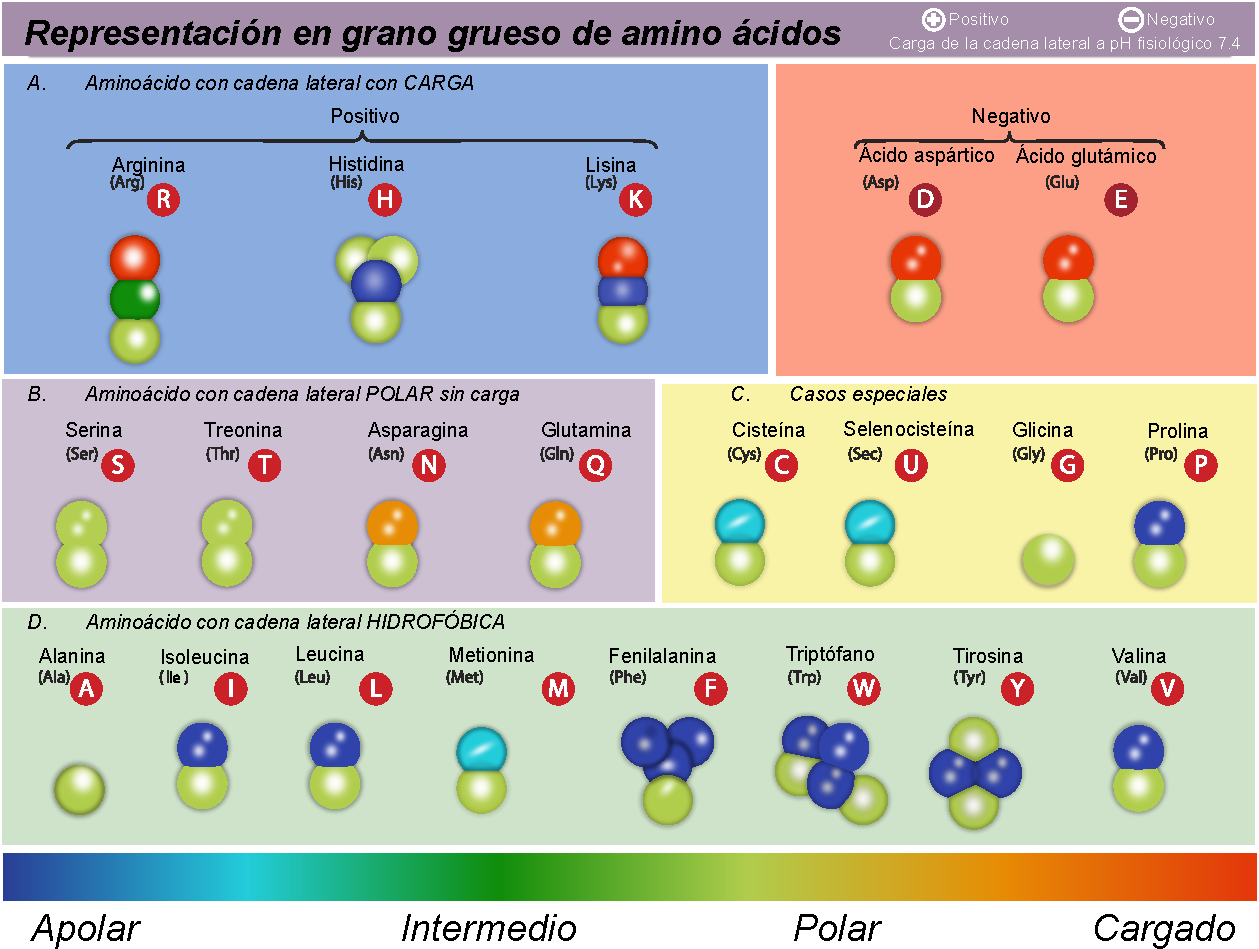
\includegraphics[width=1\linewidth, height=0.99\textheight, keepaspectratio]{fig/04_anexos/cg_aa.pdf} 
\caption[Representación en grano grueso de de los 21 amino ácidos]{Representación en grano grueso de de los 21 amino ácidos}
        \index{cg_aa}
    \label{tab:tabla_cg_aa}
\end{figure}
%%%%%%%%%%%%%%%%%%%%%%% Fin %%%%%%%%%%%%%%%%%%%%%%%%




\subsection{Campo de fuerza MARTINI}



%%%Tabla tomada de la tesis: lipid_protein_interaction...
% Please add the following required packages to your document preamble:
% \usepackage{booktabs}
% \usepackage[table,xcdraw]{xcolor}
% Beamer presentation requires \usepackage{colortbl} instead of \usepackage[table,xcdraw]{xcolor}
\begin{table}[]
\centering
\caption{Mapeo de la cadena lateral de amino ácidos con el campo de fuerza MARTINI v2.1. Partículas en grano grueso (CG)}
\label{tab:cg_particles}
\begin{tabular}{@{}ll@{}}
\toprule
\rowcolor[HTML]{EFEFEF} 
\multicolumn{1}{l}{\cellcolor[HTML]{EFEFEF}Cadena lateral} & \multicolumn{1}{l}{\cellcolor[HTML]{EFEFEF}Partícula GG} \\ \midrule
Leu/Ile  & C1              \\
Val/Pro  & C2              \\
Met/Cys  & P1              \\
Ser/Thr  & P5              \\
Gln      & P4              \\
Asp$^\text{--1}$ & Qa              \\
Asp$^0$  & P3              \\
Glu$^\text{--1}$ & Qa              \\
Glu$^0$  & P1              \\
Arg$^\text{--1}$ & N0-Qd           \\
Arg$^0$  & N0-P4            \\
Lys$^\text{--1}$ & C3-Qd           \\
Lys$^0$  & C3-P1           \\
His      & SC4-SP1-SP1     \\
Phe      & SC4-SC4-SC4     \\
Tyr      & SC4-SC4-SP1     \\
Trp      & SC4-SP1-SC4-SC4 \\ \bottomrule
\end{tabular}
\end{table}



%%%%%%%%%%% Figura %%%%%%%%%%%%
\begin{figure}[]
    \centering
	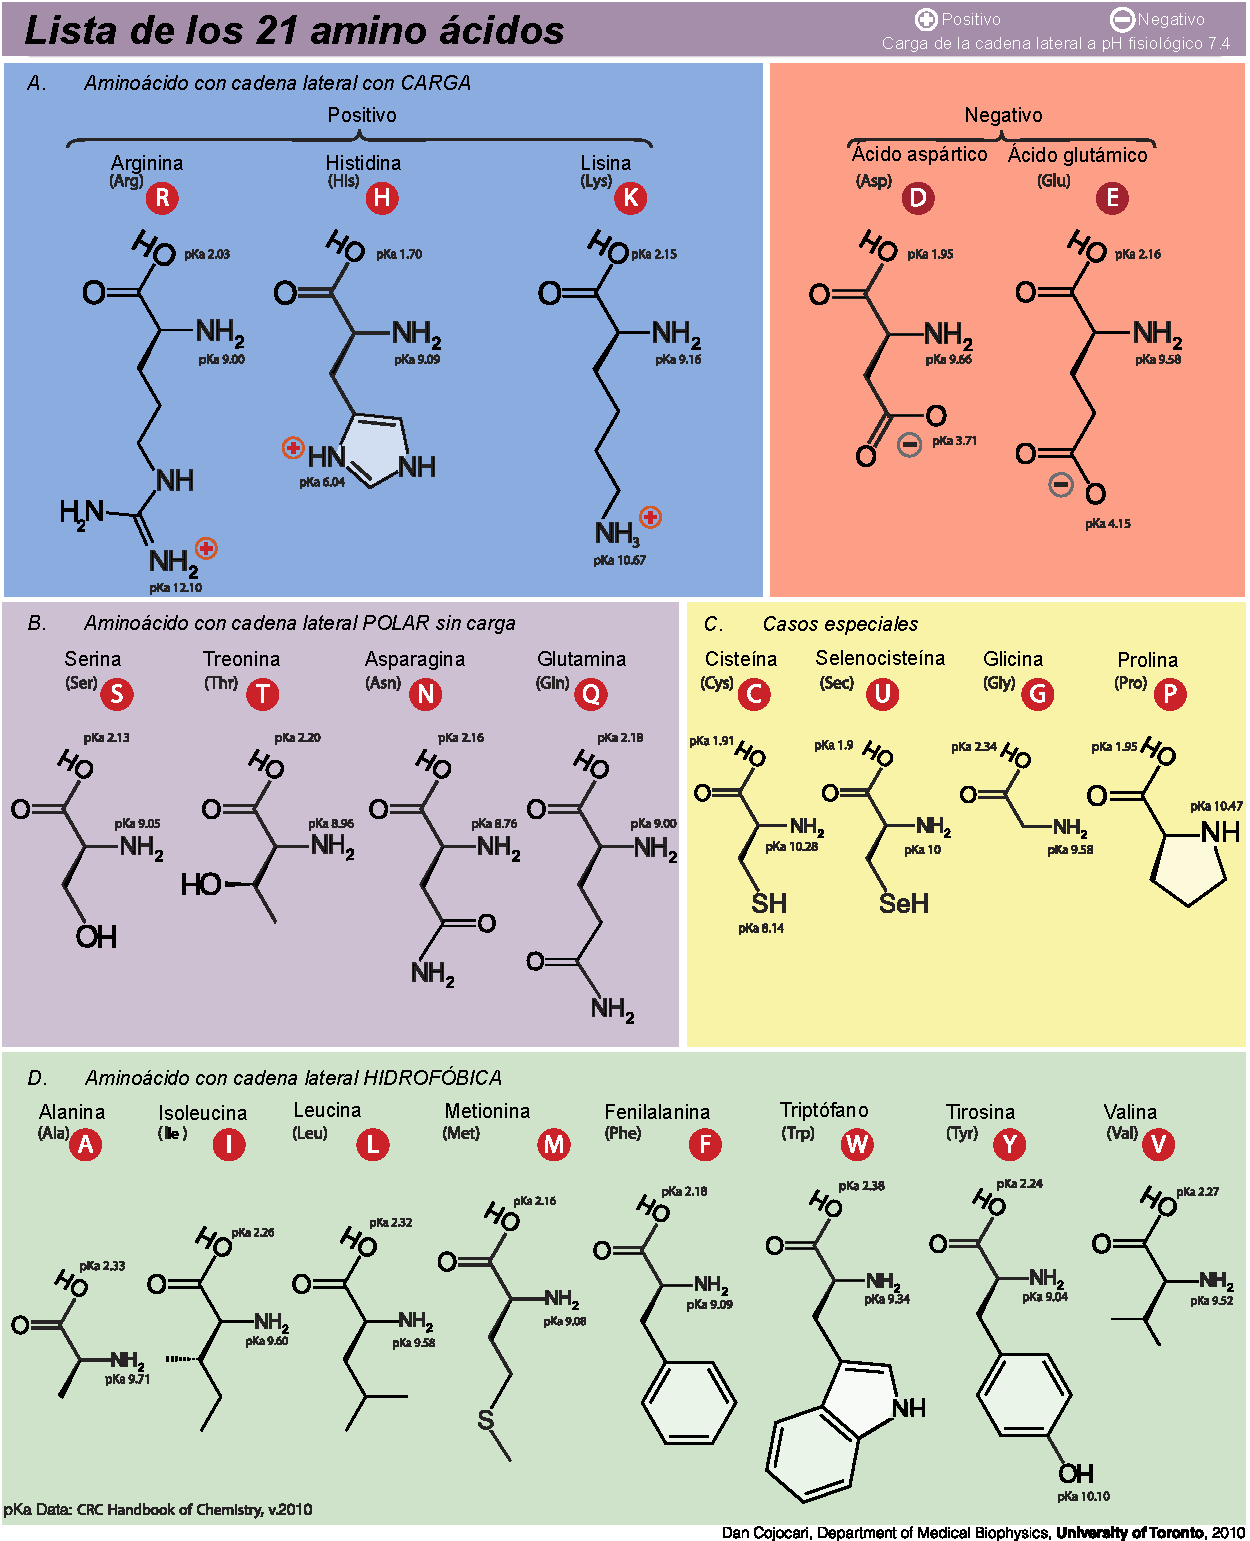
\includegraphics[width=1\linewidth, height=0.99\textheight, keepaspectratio]{fig/04_anexos/tabla_aa.pdf} 
\caption[]{Lista de los 21 amino ácidos, estructura química, código de letras, agrupados por propiedades fisicoquímicas. Figura adaptada por Dancojocari bajo \textit{Creative Commons} (CC BY-SA 3.0 - \url{https://commons.wikimedia.org/wiki/File:Amino_Acids.svg}).}
        \index{tabla_aa}
    \label{tab:tabla_aa}
\end{figure}
%%%%%%%%%%%%%%%%%%%%%%% Fin %%%%%%%%%%%%%%%%%%%%%%%%

\end{appendix}
%\begin{appendix}

\chapter{Anexo: Nombrar el anexo A de acuerdo con su contenido}\label{AnexoA}
Los Anexos son documentos o elementos que complementan el cuerpo de la tesis o trabajo de investigaci\'{o}n y que se relacionan, directa o indirectamente, con la investigaci\'{o}n, tales como acetatos, cd, normas, etc.\\

\chapter{Anexo: Nombrar el anexo B de acuerdo con su contenido}
A final del documento es opcional incluir \'{\i}ndices o glosarios. \'{E}stos son listas detalladas y especializadas de los t\'{e}rminos, nombres, autores, temas, etc., que aparecen en el mismo. Sirven para facilitar su localizaci\'{o}n en el texto. Los \'{\i}ndices pueden ser alfab\'{e}ticos, cronol\'{o}gicos, num\'{e}ricos, anal\'{\i}ticos, entre otros. Luego de cada palabra, t\'{e}rmino, etc., se pone coma y el n\'{u}mero de la p\'{a}gina donde aparece esta informaci\'{o}n.\\

\chapter{Anexo: Nombrar el anexo C de acuerdo con su contenido}
MANEJO DE LA BIBLIOGRAF\'{I}A: la bibliograf\'{\i}a es la relaci\'{o}n de las fuentes documentales consultadas por el investigador para sustentar sus trabajos. Su inclusi\'{o}n es obligatoria en todo trabajo de investigaci\'{o}n. Cada referencia bibliogr\'{a}fica se inicia contra el margen izquierdo.\\

La NTC 5613 establece los requisitos para la presentaci\'{o}n de referencias bibliogr\'{a}ficas citas y notas de pie de p\'{a}gina. Sin embargo, se tiene la libertad de usar cualquier norma bibliogr\'{a}fica de acuerdo con lo acostumbrado por cada disciplina del conocimiento. En esta medida es necesario que la norma seleccionada se aplique con rigurosidad.\\

Es necesario tener en cuenta que la norma ISO 690:1987 (en Espa\~{n}a, UNE 50-104-94) es el marco internacional que da las pautas m\'{\i}nimas para las citas bibliogr\'{a}ficas de documentos impresos y publicados. A continuaci\'{o}n se lista algunas instituciones que brindan par\'{a}metros para el manejo de las referencias bibliogr\'{a}ficas:\\

\begin{center}
\centering%
\begin{tabular}{|p {7.5 cm}|p {7.5 cm}|}\hline
\arr{Instituci\'{o}n}&Disciplina de aplicaci\'{o}n\\\hline%
Modern Language Association (MLA)&Literatura, artes y humanidades\\\hline%
American Psychological Association (APA)&Ambito de la salud (psicolog\'{\i}a, medicina) y en general en todas las ciencias sociales\\\hline
Universidad de Chicago/Turabian &Periodismo, historia y humanidades.\\\hline
AMA (Asociaci\'{o}n M\'{e}dica de los Estados Unidos)&Ambito de la salud (psicolog\'{\i}a, medicina)\\\hline
Vancouver &Todas las disciplinas\\\hline
Council of Science Editors (CSE)&En la actualidad abarca diversas ciencias\\\hline
National Library of Medicine (NLM) (Biblioteca Nacional de Medicina)&En el \'{a}mbito m\'{e}dico y, por extensi\'{o}n, en ciencias.\\\hline
Harvard System of Referencing Guide &Todas las disciplinas\\\hline
JabRef y KBibTeX &Todas las disciplinas\\\hline
\end{tabular}
\end{center}

Para incluir las referencias dentro del texto y realizar lista de la bibliograf\'{\i}a en la respectiva secci\'{o}n, puede utilizar las herramientas que Latex suministra o, revisar el instructivo desarrollado por el Sistema de Bibliotecas de la Universidad Nacional de Colombia\footnote{Ver: www.sinab.unal.edu.co}, disponible en la secci\'{o}n "Servicios", opci\'{o}n "Tr\'{a}mites" y enlace "Entrega de tesis".

\end{appendix}

\addcontentsline{toc}{chapter}{\numberline{}Bibliografía}
\bibliographystyle{plain}
\bibliography{biblio}

\end{document}